\documentclass[12pt,letterpaper]{article}   % Tamaño 12, papel carta

% Paquetes esenciales
\usepackage[spanish]{babel}        % Idioma español
\usepackage[utf8]{inputenc}        % Codificación UTF-8
\usepackage[T1]{fontenc}           % Codificación de fuente
\usepackage{setspace}              % Control del interlineado
\usepackage[margin=2.5cm]{geometry}% Márgenes de 2.5cm
\usepackage{parskip}               % Evita sangrías y añade espacio entre párrafos

\usepackage{graphicx}
\usepackage{titling}               % Para personalizar la portada
\usepackage{amsmath}               % Para mates
\usepackage{amssymb}               % Letras de mates
\usepackage{hyperref}              % Para el índice

\usepackage{amsfonts}
\usepackage{pgfplots}
\usepackage{booktabs}

% Interlineado 1.5
\onehalfspacing

% Justificación del texto
\usepackage{ragged2e}
\justifying

% No sangría en párrafos
\setlength{\parindent}{0pt}

% Numerado de pagina arriba a la derecha
\usepackage{fancyhdr}
\pagestyle{fancy}
\fancyhf{} % Limpia encabezados y pies predeterminados
\fancyhead[R]{\thepage} % Número de página en encabezado derecha
\renewcommand{\headrulewidth}{0pt} % Elimina la línea bajo el encabezado

% Que los titulos de las secciónes tengan el mismo tamaño
\usepackage{titlesec}

% Configuración de \section
\titlespacing*{\section}{0pt}{2ex plus 1ex minus .2ex}{-0.5ex} 
\titleformat{\section}[block]{\normalfont\normalsize\bfseries}{\thesection}{1em}{}

\titlespacing*{\subsection}{0pt}{2ex plus 1ex minus .2ex}{-0.5ex} 
\titleformat{\subsection}[block]{\normalfont\normalsize\bfseries}{\thesubsection}{1em}{}

\titlespacing*{\subsubsection}{0pt}{2ex plus 1ex minus .2ex}{-0.5ex} 
\titleformat{\subsubsection}[block]{\normalfont\normalsize\bfseries}{\thesubsubsection}{1em}{}

\titlespacing*{\paragraph}{0pt}{2ex plus 1ex minus .2ex}{-0.5ex} 
\titleformat{\paragraph}[block]{\normalfont\normalsize\bfseries}{\paragraph}{1em}{}

\titlespacing*{\subparagraph}{0pt}{2ex plus 1ex minus .2ex}{-0.5ex} 
\titleformat{\subparagraph}[block]{\normalfont\normalsize\bfseries}{\subparagraph}{1em}{}


% Consola
\usepackage{listings}
\usepackage{xcolor}
\definecolor{consolegray}{gray}{0.95}
\definecolor{consoleborder}{gray}{0.7}
\lstnewenvironment{smallconsole}[1][]{
  \lstset{
    basicstyle=\ttfamily\tiny, 
    backgroundcolor=\color{consolegray},
    frame=single,
    rulecolor=\color{consoleborder},
    breaklines=true,
    columns=fullflexible,
    showstringspaces=false,
    captionpos=b,
    xleftmargin=1em,
    xrightmargin=1em,
    aboveskip=1em,
    belowskip=1em,
    #1 % ← Para pasar opciones como caption
  }
}{}


% Tamaño de las captions
\usepackage{caption}
\captionsetup{font=scriptsize}

% Multicolumnas
\usepackage{multicol}
\usepackage{listings}
\usepackage{xcolor}
\usepackage{multicol}

\definecolor{consolegray}{gray}{0.95}
\definecolor{consoleborder}{gray}{0.7}

% Define el estilo una vez
\lstdefinestyle{smallconsolestyle}{
  basicstyle=\ttfamily\tiny,
  breaklines=true,
  columns=fullflexible,
  showstringspaces=false,
  captionpos=b,
  xleftmargin=0em,
  xrightmargin=0em,
  aboveskip=1em,
  belowskip=1em,
  frame=none,
  backgroundcolor=\color{white},
  rulecolor=\color{white}
}




% Configuración para usar el punto como separador decimal
\renewcommand{\theequation}{\arabic{equation}}



\begin{document}




% ----------------------------------
% Portada
% ----------------------------------
\begin{titlepage}
    \begin{center}
        \vspace*{2cm}
        \textbf{Análisis de Series de Tiempo para la Precipitación en Puebla}\\[2cm]

        Heriberto Espino Montelongo - 175199\\[0.5cm]
        Universidad de las Américas Puebla\\[0.5cm]
        P25-LEC4032-2: Econometría II\\[0.5cm]
        Dra. Daniela Cortés Toto\\[0.5cm]
        30 de abril de 2025\\
    \end{center}
    \vfill
\end{titlepage}


% ----------------------------------
% Contenido del documento
% ----------------------------------


\pagenumbering{Roman}
\setcounter{page}{1}
\tableofcontents
\newpage


% A partir de aquí empieza la numeración arábiga desde 1
\pagenumbering{arabic}
\setcounter{page}{1}
\section{Introducción}
La precipitación es un elemento fundamental del clima que influye directamente en la disponibilidad de agua, la planificación urbana y la actividad económica y social de la ciudad. En regiones como Puebla, donde se combina una diversidad climática con una fuerte dependencia de los recursos hídricos, entender los patrones de precipitación se vuelve crucial para una adecuada toma de decisiones en múltiples sectores.
En este trabajo se realiza un análisis estadístico de la precipitación mensual registrada en la estación meteorológica Puebla (DGE), ubicada en las coordenadas 19.0000°N, 98.1833°O. Los datos fueron obtenidos del repositorio de la National Oceanic and Atmospheric Administration (NOAA) y abarcan el periodo comprendido entre septiembre de 1952 y diciembre de 2009. A partir de esta serie histórica, se busca modelar los patrones de comportamiento estacional y de tendencia, así como generar pronósticos que permitan anticipar el comportamiento futuro de la precipitación en la región.



\subsection{Planteamiento del problema}
La precipitación es una variable climática de alta relevancia para el funcionamiento de los sistemas económicos, sociales, alimenticios, entre otros. Su variabilidad, tanto en magnitud como en frecuencia, puede tener efectos significativos sobre la economía local, el bienestar social y la sostenibilidad de los ecosistemas urbanos y rurales. Los cambios abruptos o sostenidos en los patrones de precipitación pueden derivar en fenómenos extremos como sequías prolongadas o inundaciones severas, afectando directamente la producción agrícola, la disponibilidad de agua potable, el funcionamiento de la infraestructura hidráulica y la salud pública.

En contextos urbanos, una precipitación intensa y mal gestionada puede colapsar los sistemas de drenaje, deteriorar la infraestructura vial, aumentar la vulnerabilidad de asentamientos irregulares y agravar condiciones socioeconómicas preexistentes. En entornos rurales, la dependencia directa de la lluvia para actividades agropecuarias implica que cualquier alteración en los patrones de precipitación puede traducirse en pérdidas económicas, inseguridad alimentaria y desplazamientos poblacionales.

Dado que la precipitación muestra una estructura temporal compleja con componentes estacionales y posibles tendencias de largo plazo, es fundamental desarrollar modelos que permitan describir su comportamiento histórico y anticipar su evolución futura. Estas herramientas son clave para mejorar la toma de decisiones en sectores sensibles al clima, optimizar la asignación de recursos hídricos, diseñar políticas públicas resilientes y fortalecer la planificación territorial frente a escenarios de cambio climático.

En este contexto, surge la siguiente pregunta de investigación:
\textit{¿Cómo se ha comportado la precipitación mensual en Puebla y qué tipo de modelo es más adecuado para explicar su dinámica temporal y generar predicciones confiables para los años siguientes?}



\subsection{Objetivo general}
Desarrollar un análisis para la serie de tiempo de la precipitación mensual en Puebla (1952–2009), con el propósito de caracterizar su dinámica histórica, incluyendo patrones estacionales, tendencias de largo plazo y eventos extremos, y proponer un modelo que ofrezca pronósticos confiables, contribuyendo así a la toma de decisiones en sectores sociales y económicos sensibles a la variabilidad climática.


\subsection{Objetivos específicos}
Para alcanzar el objetivo general, se propone navegar por distintas metodologías y comparar los resultados. Se buscará identificar patrones estacionales u otro tipo de tendencias. Con base en estas características, se probarán distintos modelos, como modelos ARIMA  con componentes estacionales, con el objetivo de encontrar el que mejor se ajuste a los datos observados. Una vez seleccionado el modelo óptimo, se procederá a realizar pronósticos sobre el comportamiento de la precipitación. 



\subsection{Justificación}
La precipitación es un factor climático fundamental que incide directamente en múltiples dinámicas sociales y económicas. Su variabilidad temporal y espacial afecta de manera significativa sectores estratégicos como la agricultura, la gestión de los recursos hídricos, la planificación territorial y la prevención de desastres naturales. Como ejemplos se encuentran la producción agrícola, que depende de las lluvias, lo que condiciona tanto el rendimiento como la viabilidad de distintos cultivos; de igual forma, la infraestructura hidráulica y los sistemas de abastecimiento de agua, que requieren de una planificación precisa basada en patrones de precipitación confiables.

Ante este panorama, se busca desarrollar una herramienta que permita describir y predecir el comportamiento mensual de la precipitación. Teniendo como propósito mejorar la toma de decisiones en sectores sensibles al clima, facilitando la formulación de toma de decisiones, fortaleciendo la capacidad de respuesta y adaptación ante eventos extremos, como sequías prolongadas o lluvias torrenciales que derivan en inundaciones.


\subsection{Hipótesis}
Se plantea la hipótesis de que la precipitación mensual en la ciudad de Puebla tiene una periodicidad anual (o de cada doce meses), así como una posible estabilidad en su tendencia de largo plazo, sujeta a perturbaciones atribuibles a la variabilidad climática y a la ocurrencia de fenómenos extremos. Se espera, además, una fuerte dependencia temporal, en la cual los valores actuales de precipitación están correlacionados con observaciones previas, tanto de meses recientes como de años anteriores. Bajo este supuesto, se considera que un modelo ARIMA con compontentes estacionales será adecuado para capturar la estructura temporal de la serie, modelar sus componentes, y generar predicciones con utilidad práctica para la toma de decisiones sensibles respecto a aspectos climáticos.

\newpage

\section{Desarrollo}
Para estudiar el comportamiento de la precipitación en la ciudad de Puebla a lo largo del tiempo, se analizará una serie mensual que representa los niveles de precipitación acumulada por mes en milímetros. Esta información fue recopilada por la NOAA a través de su red de estaciones climatológicas, en particular la estación identificada como Puebla (DGE), El periodo que abarca la serie es de septiembre de 1952 a diciembre de 2009. A continuación, se muestra el gráfico de la precipitación mensual durante todo el periodo observado.

\begin{figure}[h!]
    \centering
    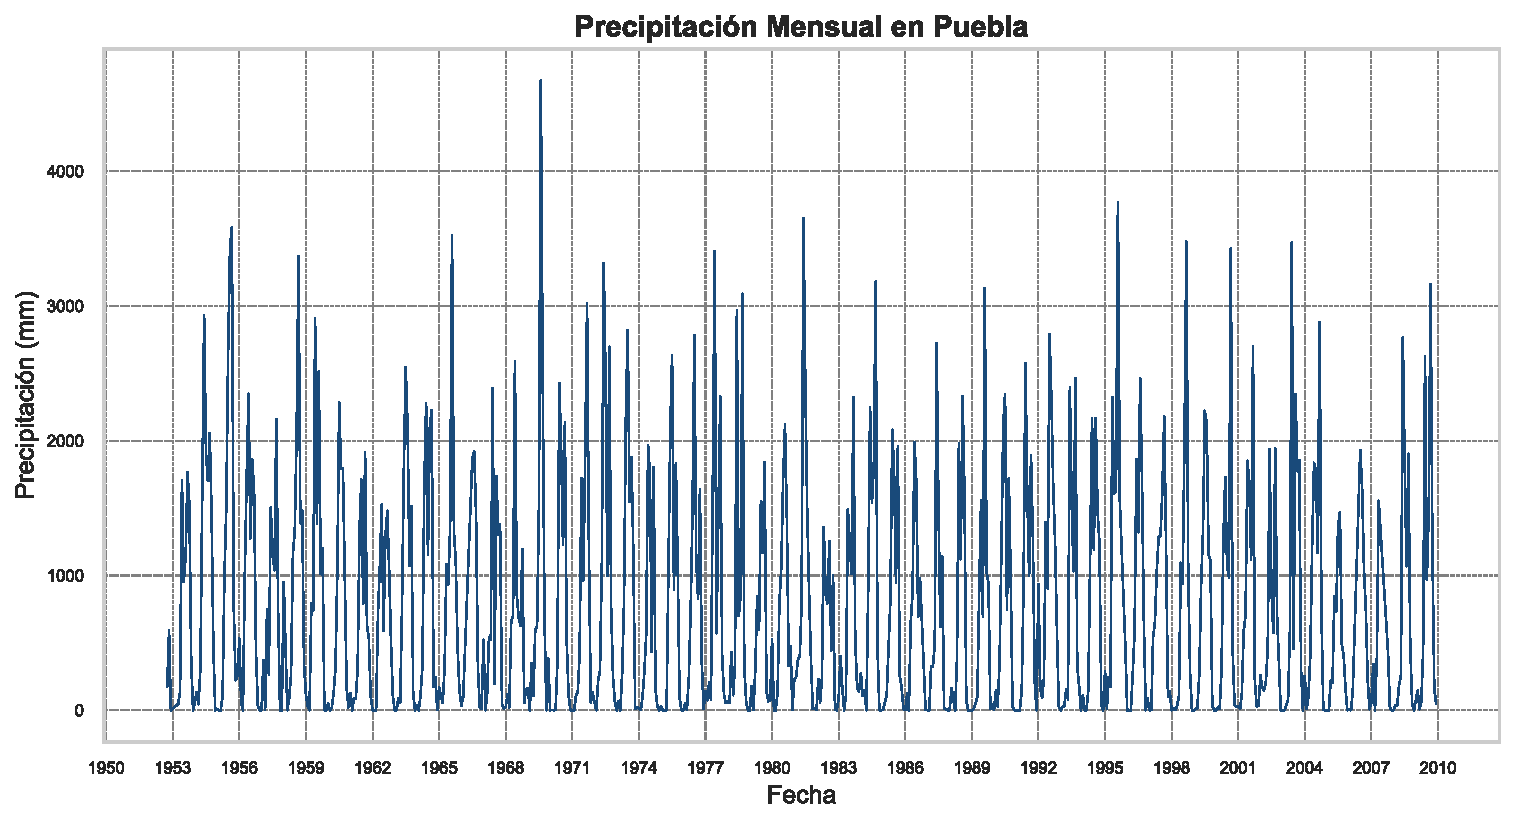
\includegraphics[width=0.7\textwidth]{imagenes/01-01-precipitacion.pdf}
    \caption{\textit{Elaboración Propia}. Descripción de la imagen.}
    \label{fig:mi_imagen}
\end{figure}

Para una mejor visualización se muestran los últimos 10 años de la serie

\begin{figure}[h!]
    \centering
    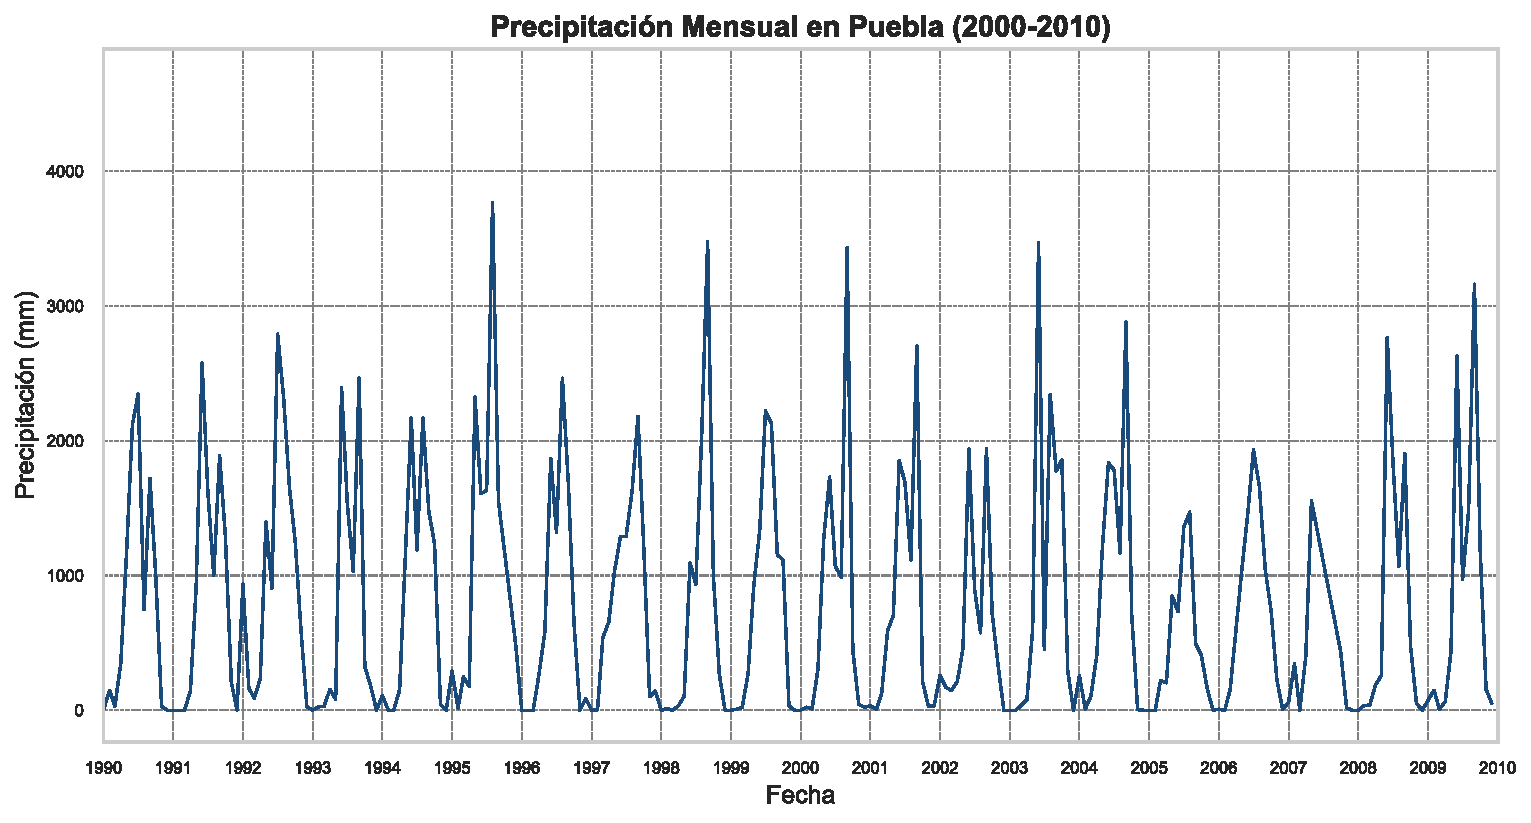
\includegraphics[width=0.7\textwidth]{imagenes/01-02-precipitacion-zoom.pdf}
    \caption{\textit{Elaboración Propia}. Descripción de la imagen.}
    \label{fig:mi_imagen}
\end{figure}


 Como puede apreciarse, los p-valores presentan una marcada estacionalidad, con picos de precipitación concentrados en los meses de verano, durante el principio de la segunda mitad de cada año. Esta estacionalidad responde a los ciclos climáticos típicos de la región central de México, donde predominan las lluvias en la temporada de verano.


\subsection{Partición de la Serie para su Análisis}
Antes de comenzar a trabajar con la serie temporal, y considerando que uno de los objetivos principales de este trabajo es la actualización del pronóstico y la comparación de resultados, no serán utilizados los últimos 12 meses de la serie. Es importante destacar que a partir de este momento solo se trabajará con esta porción de la serie, hasta que se generen los pronósticos y únicamente será utilizada en modo de comparación con los datos de la serie original, posteriormente, actualizaremos el pronóstico y repetiremos la comparación.

\subsection{Serie Sin Transformaciones}
En esta sección se analiza la serie original de precipitación mensual sin aplicar transformaciones, más allá de la estandarización, que no cambia la distribución de los datos. La estandarización se realizó con el objetivo de facilitar la comparación con modelos entrenados sobre versiones transformadas de la serie, asegurando así que métricas como el log-likelihood y el AIC sean directamente comparables entre modelos.

\textbf{Verificación de Estacionariedad de la Serie}


Para verificar la estacionariedad de la serie de precipitación mensual en Puebla, se aplicó la prueba de Dickey-Fuller aumentada (ADF). El resultado obtenido fue:
\begin{itemize}
    \item El estadístico de prueba es -6.15,
    \item El p-valor es $7.58 \times 10^{-8}$,
    \item Los valores críticos a los niveles del 1\%, 5\% y 10\% son -3.44, -2.86 y -2.57.
\end{itemize}


Dado que el p-valor es mucho menor que 0.05, se rechaza la hipótesis nula. Esto indica que la serie de precipitación mensual en Puebla es estacionaria, por lo que no sería necesario aplicar diferenciación o transformaciones.

\textbf{Autocorrelaciones Simples y Autocorrelaciones Parciales
}

Los gráficos de Autocorrelaciones Simples (FAC) y Autocorrelaciones Parciales (FACP) muestran el comportamiento de la serie de tiempo de precipitación mensual en Puebla, con un retraso de hasta 48 observaciones. En el caso de la FAC, se observa que las autocorrelaciones no decaen rápidamente, lo que sugiere que la serie tiene una dependencia temporal significativa en varios retrasos. Esto puede indicar que la serie no es completamente estacionaria y se justifica la necesidad de aplicar una diferencia estacional.

\begin{figure}[ht]
    \centering
    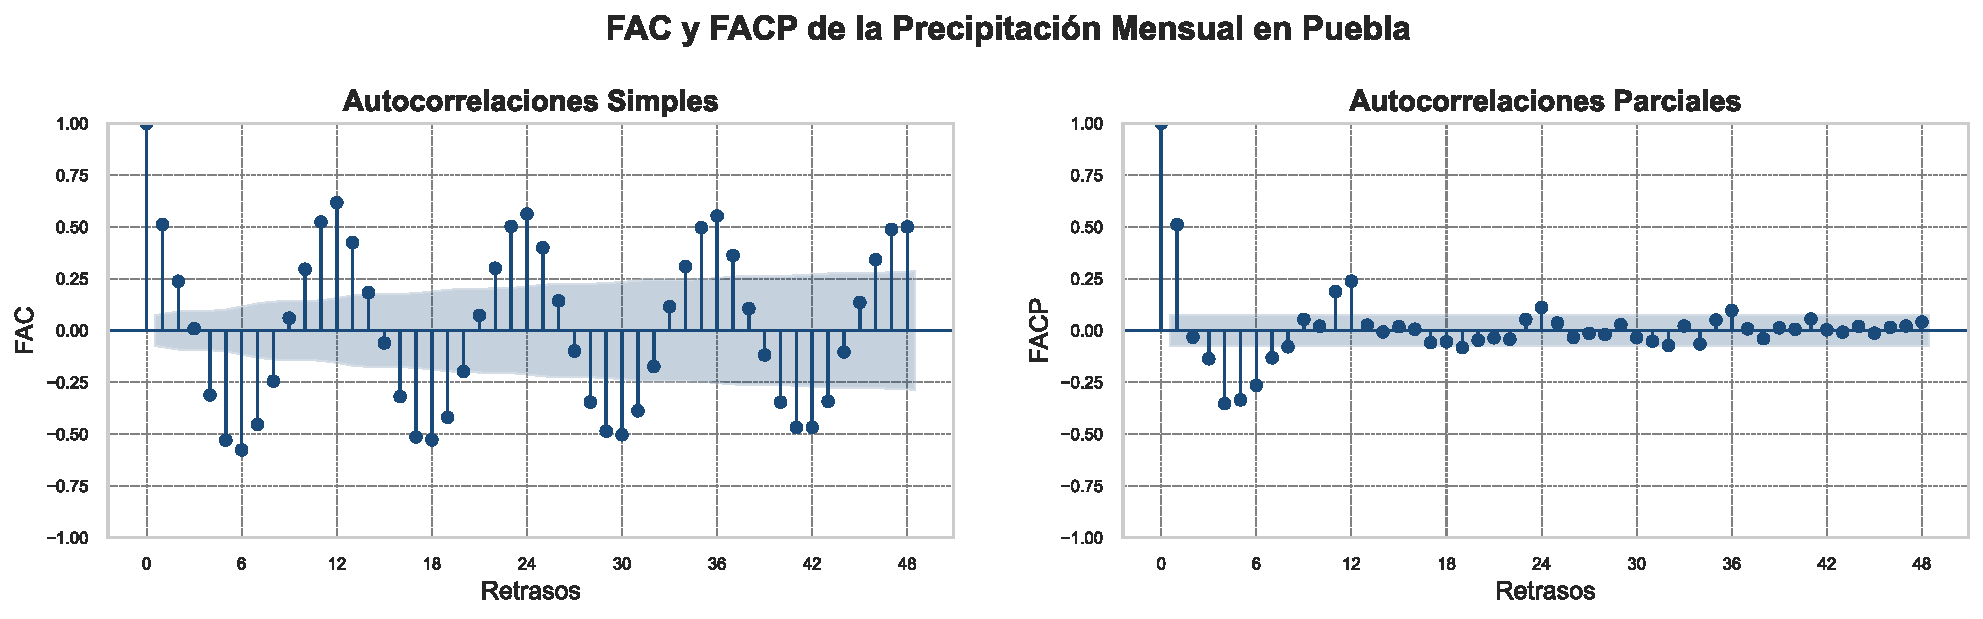
\includegraphics[width=0.8\textwidth]{imagenes/02-01-fac-facp-serie.pdf}
    \caption{\textit{Elaboración Propia}. FAC y FACP de la serie de Precipitación Mensual en Puebla}
\end{figure}

Los valores significativos de autocorrelación para la serie original fueron los siguientes:
\begin{multicols}{5}
\scriptsize
\begin{itemize}
    \item $r_1$: 0.511
    \item $r_2$: 0.238
    \item $r_4$: -0.311
    \item $r_5$: -0.529
    \item $r_6$: -0.577
    \item $r_7$: -0.454
    \item $r_8$: -0.244
    \item $r_{10}$: 0.296
    \item $r_{11}$: 0.524
    \item $r_{12}$: 0.617
    \item $r_{13}$: 0.424
    \item $r_{14}$: 0.183
    \item $r_{16}$: -0.319
    \item $r_{17}$: -0.514
    \item $r_{18}$: -0.528
    \item $r_{19}$: -0.419
    \item $r_{22}$: 0.301
    \item $r_{23}$: 0.503
    \item $r_{24}$: 0.563
\end{itemize}
\end{multicols}{}

\vspace{1em}

\normalsize
Mientras que para las autocorrelaciones parciales los valores significativos fueron:
\begin{multicols}{5}
\scriptsize
\begin{itemize}
    \item $\rho_1$: 0.512
    \item $\rho_3$: -0.137
    \item $\rho_4$: -0.356
    \item $\rho_5$: -0.339
    \item $\rho_6$: -0.270
    \item $\rho_7$: -0.137
    \item $\rho_8$: -0.082
    \item $\rho_{11}$: 0.194
    \item $\rho_{12}$: 0.250
    \item $\rho_{19}$: -0.092
    \item $\rho_{24}$: 0.124
\end{itemize}
\end{multicols}{}

\vspace{1em}

\normalsize

\subsection{Diferencias Estacionales de la Serie Sin Transformar}

Aunque la serie fue declarada estacionaria mediante la prueba ADF en su forma original, las autocorrelaciones simples decrecían muy lentamente, lo cual sugiere la presencia de estacionalidad. 



\subsubsection{Primera Diferencia Estacional}

 Se aplicó una diferencia estacional de orden \( D = 1 \) con periodicidad anual \( s = 12 \):

\[
\nabla_{12} X_t = X_t - X_{t-12}
\]

Esta transformación busca eliminar la estacionalidad anual observada en la serie, resultando en la siguiente:


\begin{figure}[ht]
    \centering
    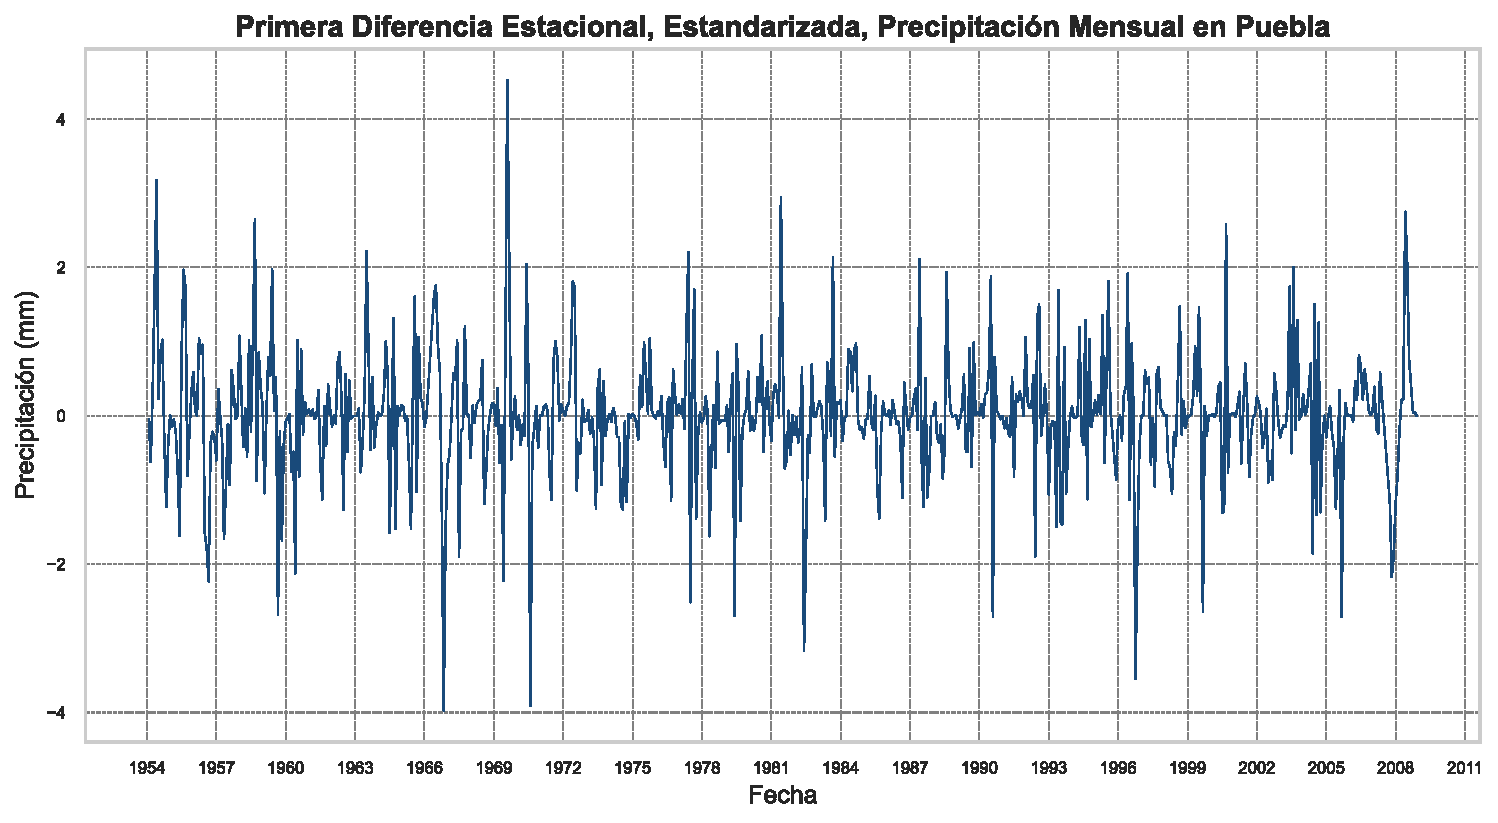
\includegraphics[width=0.8\textwidth]{imagenes/03-01-primera-diferencia-estacional-precipitacion.pdf}
    \caption{\textit{Elaboración Propia}. Primera Diferencia Estacional, Precipitación Mensual en Puebla}
\end{figure}


\textbf{Verificación de Estacionariedad de la Serie}

La serie resultante, fue evaluada nuevamente con la prueba de Dickey-Fuller aumentada, obteniendo los siguientes resultados:

\begin{itemize}
    \item Estadístico ADF: -10.8714
    \item p-valor: $1.36 \times 10^{-19}$
    \item Valores críticos: -3.44 (1\%), -2.86 (5\%), -2.57 (10\%)
\end{itemize}

Dado que el p-valor es menor a cualquier nivel de significancia, se rechaza la hipótesis nula de no estacionariedad. Por tanto, concluimos que la serie diferenciada es estacionaria. 

\textbf{Autocorrelaciones Simples y Autocorrelaciones Parciales
}

Para analizar la dependencia temporal en la serie, se graficaron la FAC y la FACP de la serie:

\begin{figure}[ht]
    \centering
    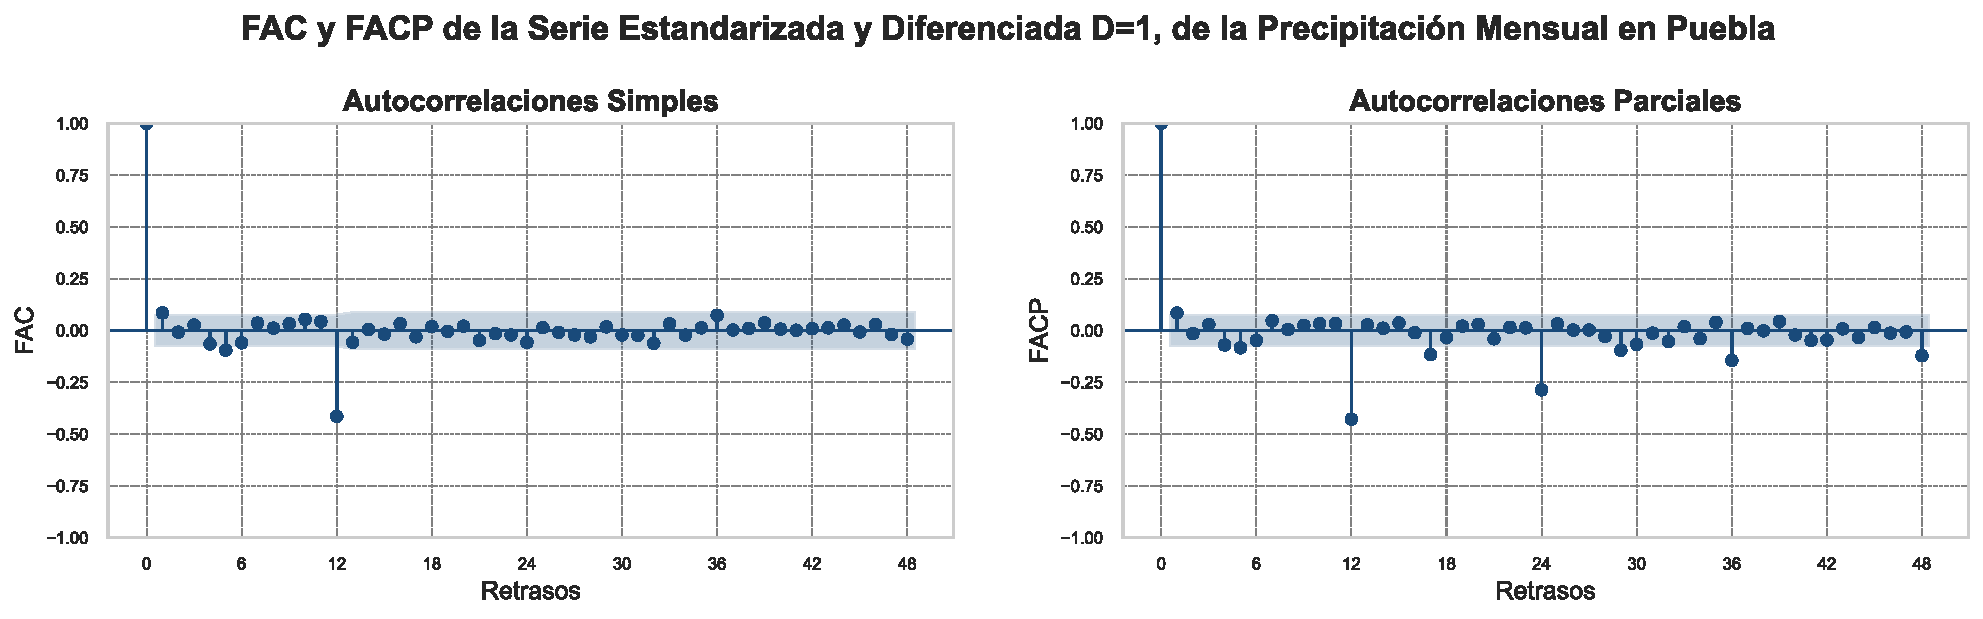
\includegraphics[width=0.8\textwidth]{imagenes/03-02-fac-facp-serie-D1.pdf}
    \caption{\textit{Elaboración Propia}. FAC y FACP de la Primera Diferencia Estacional}
\end{figure}

Los valores significativos de autocorrelación para la primera diferencia estacional fueron los siguientes: \begin{multicols}{5} \scriptsize \begin{itemize} \item $r_1$: 0.085 \item $r_5$: -0.095 \item $r_{12}$: -0.414 \item $r_{69}$: 0.138 \item $r_{73}$: -0.113 \item $r_{82}$: -0.099 \end{itemize} \end{multicols}{}

\vspace{1em}

\normalsize Mientras que para las autocorrelaciones parciales los valores significativos fueron: \begin{multicols}{5} \scriptsize \begin{itemize} \item $\rho_1$: 0.085 \item $\rho_5$: -0.084 \item $\rho_{12}$: -0.436 \item $\rho_{17}$: -0.120 \item $\rho_{24}$: -0.301 \item $\rho_{29}$: -0.102 \item $\rho_{36}$: -0.160 \item $\rho_{48}$: -0.140 \item $\rho_{57}$: -0.092 \item $\rho_{60}$: -0.124 \item $\rho_{61}$: 0.138 \item $\rho_{69}$: 0.103 \item $\rho_{72}$: -0.095 \item $\rho_{82}$: -0.080 \item $\rho_{85}$: -0.082 \item $\rho_{93}$: 0.092 \end{itemize} \end{multicols}{}



Esto indica que, si bien, la diferencia estacional eliminó la mayor parte de la dependencia temporal, persisten algunos retrasos con influencia significativa, lo cual será considerado en el ajuste del modelo ARIMA. También se comparará con otras diferencias.


    \subsubsection{Segunda Diferencia Estacional}


Tras aplicar una segunda diferencia estacional con periodicidad $s=12$ a la serie estandarizada (es decir, $\nabla_{12}^2 T(X_t)$), se analizó la estructura de autocorrelación para identificar patrones significativos en la nueva serie.

\begin{figure}[h!]
\centering
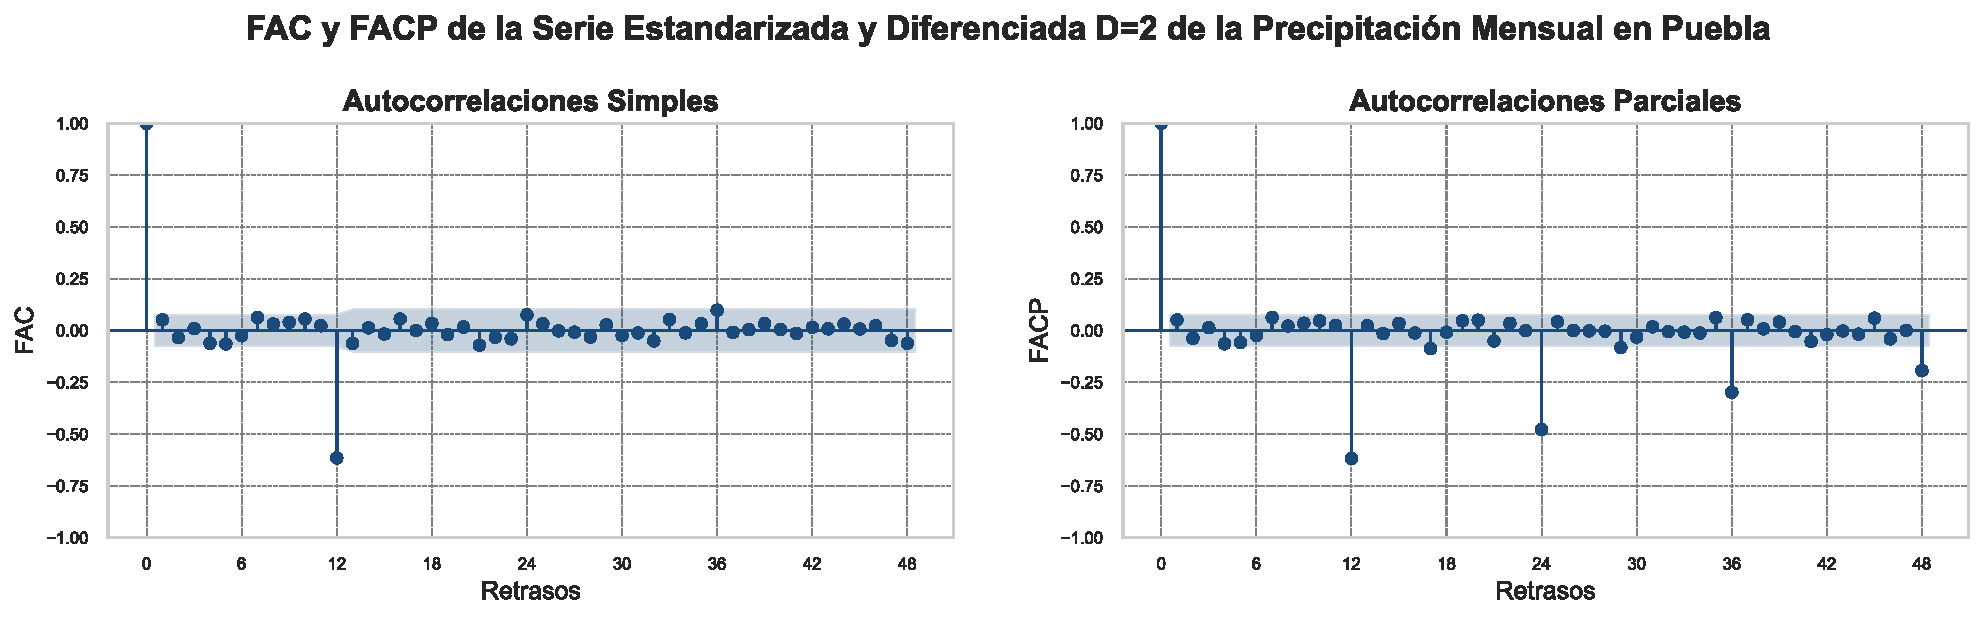
\includegraphics[width=0.95\textwidth]{imagenes/03-03-fac-facp-serie-D2.pdf}
\caption{\textit{Elaboración Propia}. FAC y FACP de la serie de precipitación mensual en Puebla, estandarizada y con segunda diferencia estacional ($D=2$, $s=12$).}
\end{figure}

Los valores significativos de autocorrelación para la segunda diferencia estacional fueron los siguientes: \begin{multicols}{5} \scriptsize \begin{itemize} \item $r_1$: 0.085 \item $r_5$: -0.095 \item $r_{12}$: -0.414 \item $r_{69}$: 0.138 \item $r_{73}$: -0.113 \item $r_{82}$: -0.099 \end{itemize} \end{multicols}{}

\vspace{1em}

\normalsize Mientras que para las autocorrelaciones parciales los valores significativos fueron: \begin{multicols}{5} \scriptsize \begin{itemize} \item $\rho_1$: 0.085 \item $\rho_5$: -0.084 \item $\rho_{12}$: -0.436 \item $\rho_{17}$: -0.120 \item $\rho_{24}$: -0.301 \item $\rho_{29}$: -0.102 \item $\rho_{36}$: -0.160 \item $\rho_{48}$: -0.140 \item $\rho_{57}$: -0.092 \item $\rho_{60}$: -0.124 \item $\rho_{61}$: 0.138 \item $\rho_{69}$: 0.103 \item $\rho_{72}$: -0.095 \item $\rho_{82}$: -0.080 \item $\rho_{85}$: -0.082 \item $\rho_{93}$: 0.092 \item $\rho_{109}$: 0.096 \item $\rho_{113}$: -0.091 \item $\rho_{119}$: 0.092 \item $\rho_{120}$: -0.136 \end{itemize} \end{multicols}{}



    \subsubsection{Tercera Diferencia Estacional}



Se aplicó una tercera diferencia estacional con periodicidad $s=12$ a la serie estandarizada de precipitación mensual. 

\begin{figure}[h!]
\centering
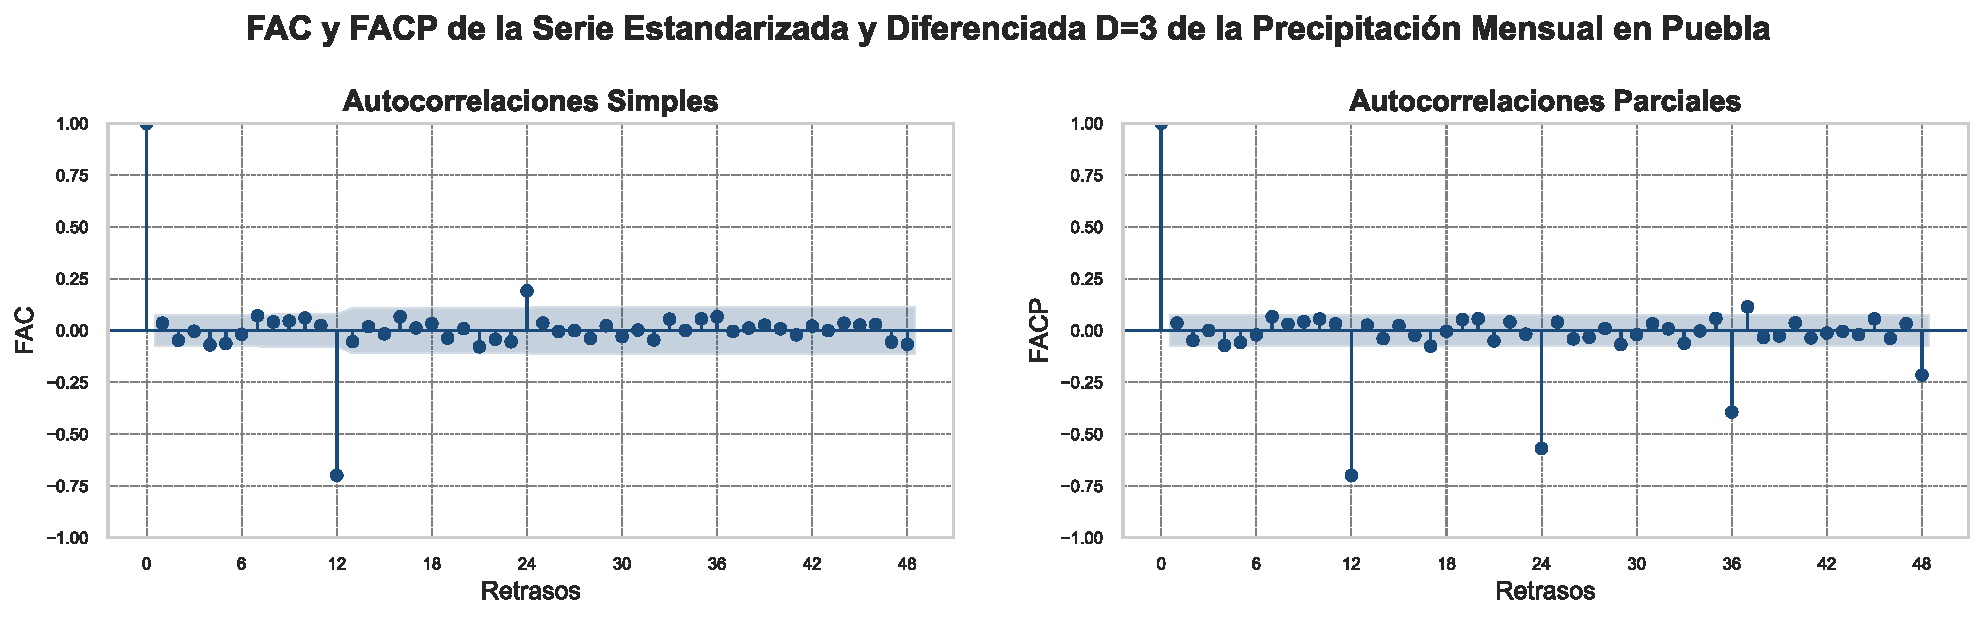
\includegraphics[width=0.95\textwidth]{imagenes/03-04-fac-facp-serie-D3.pdf}
\caption{\textit{Elaboración Propia}. FAC y FACP de la serie de precipitación mensual en Puebla, estandarizada y con tercera diferencia estacional ($D=3$, $s=12$).}
\end{figure}


\vspace{1em}


Los valores significativos de autocorrelación fueron los siguientes: \begin{multicols}{5} \scriptsize \begin{itemize} \item $r_{12}$: -0.699 \item $r_{24}$: 0.191 \item $r_{57}$: -0.131 \item $r_{69}$: 0.182 \item $r_{81}$: -0.145 \end{itemize} \end{multicols}{}

\vspace{1em}

\normalsize Mientras que para las autocorrelaciones parciales los valores significativos fueron: \begin{multicols}{5} \scriptsize \begin{itemize} \item $\rho_{12}$: -0.713 \item $\rho_{24}$: -0.617 \item $\rho_{36}$: -0.517 \item $\rho_{48}$: -0.493 \item $\rho_{52}$: 0.345 \item $\rho_{54}$: 0.331 \item $\rho_{58}$: -0.411 \item $\rho_{59}$: 1.475 \item $\rho_{60}$: 3.447 \item $\rho_{62}$: 6.763 \item $\rho_{67}$: -2.332 \item $\rho_{95}$: -6.078 \item $\rho_{107}$: -9.436 \item $\rho_{114}$: 5.771 \item $\rho_{116}$: 3.639 \end{itemize} \end{multicols}{}

Se observa una cantidad considerable de retrasos con valores extremos (por ejemplo, $\rho_{107} = -9.436$ y $\rho_{62} = 6.763$), lo que sugiere un posible sobrediferenciamiento, que genera ruido excesivo y sobreajuste en la estructura temporal.




    \subsubsection{Comparación de Desviaciones Estándar con Distintas Diferencias}



Para evaluar el efecto de las diferencias estacionales sobre la variabilidad de la serie, se comparó la desviación estándar de la serie estandarizada y sus versiones diferenciadas con $D=1$, $D=2$ y $D=3$:

\begin{figure}[h!]
\centering
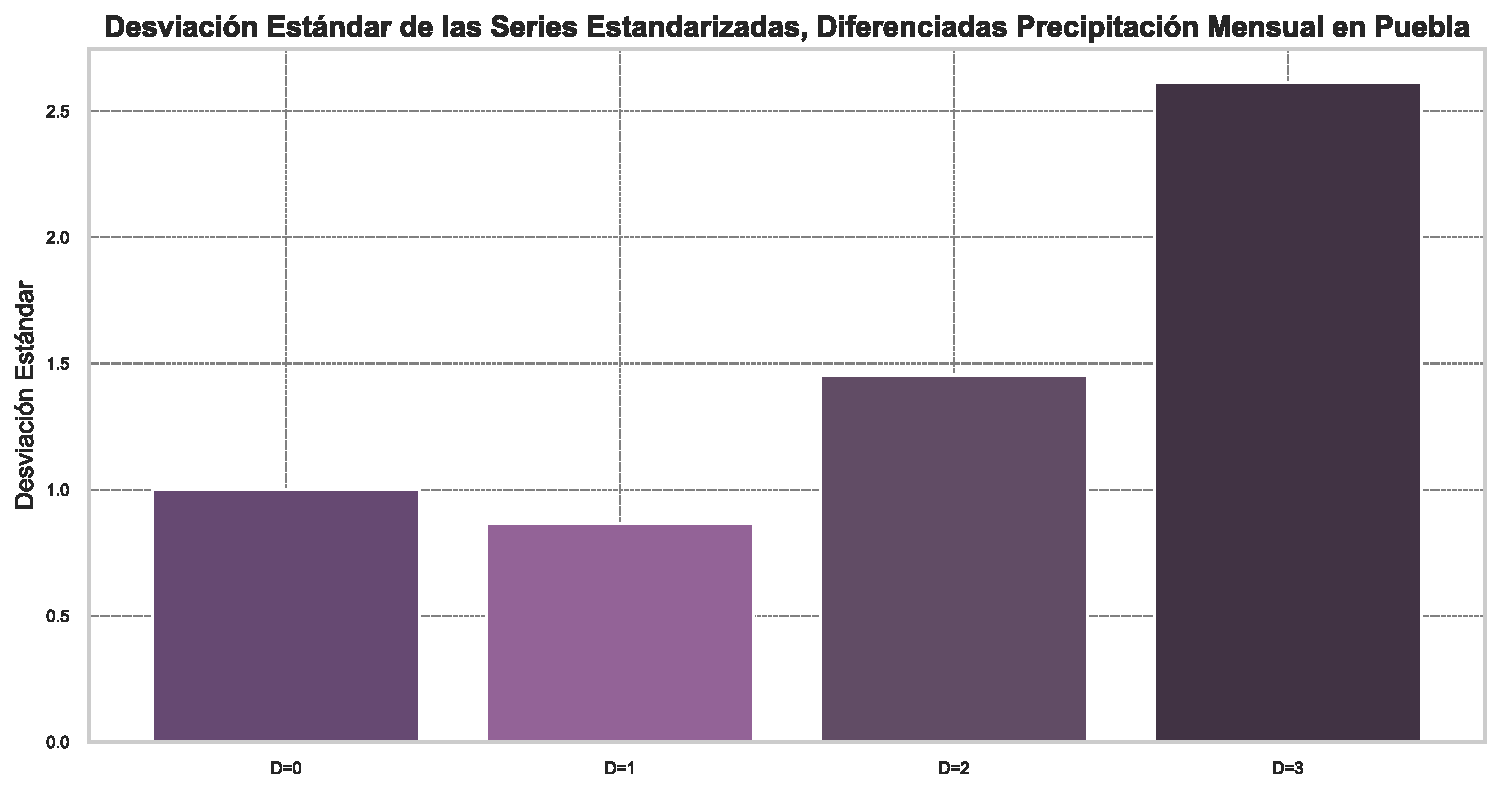
\includegraphics[width=0.75\textwidth]{imagenes/03-05-std-Ds.pdf}
\caption{\textit{Elaboración Propia}. Desviación estándar de la serie estandarizada y con diferencias estacionales de primer, segundo y tercer orden.}
\end{figure}

Se observa que la serie con menor varianza corresponde a aquella a la que se le aplicó una primera diferencia estacional. Cabe recordar que la serie original tiene varianza unitaria, ya que fue estandarizada previamente. Aunque la aplicación de diferencias estacionales tiende a reducir la varianza, el uso de tres diferencias puede resultar excesivo, lo cual se evidencia en la aparición de valores extremos en la Función de Autocorrelación Parcial (FACP), así como en la posible pérdida de estructura significativa para el modelado.
Por lo tanto, se opta por conservar únicamente la primera diferencia estacional, ya que no solo presenta la menor varianza entre las transformaciones consideradas, sino que además tiene una estructura más interpretable en su Función de Autocorrelación.






















\newpage
\subsection{Serie con Transformación}
Se utilizó la transformación Yeo-Johnson para aproximar la normalidad de los datos, lo que permite que los modelos ajustados sean más robustos y que las inferencias estadísticas sean confiables, además de ayudar a estabilizar la varianza. Esta transformación se eligió porque existen meses con precipitación igual a cero, un caso donde la transformación Box-Cox no es aplicable. Yeo-Johnson acepta valores cero sin necesidad de modificar los datos con constantes arbitrarias, preservando así su integridad y significado original.

La precipitación es una variable altamente sesgada, con muchos meses de poca o ninguna lluvia y pocos meses con lluvias abundantes. Esta transformación corrige la asimetría y acerca la distribución a una normal, mejorando los supuestos de los modelos estadísticos y aumentando la precisión en predicciones y simulaciones.

Además, la precipitación presenta varianza heterogénea, con meses en que la lluvia varía mucho respecto a otros. La transformación Yeo-Johnson contribuye a esta estabilización de la varianza.

A continuación, se muestra la definición matemática de la transformación Yeo-Johnson, como se encuentra en la literatura estadística (propuesta por Ingram Olkin y I. Paul Yeo \& R. J. Johnson en 2000).

Sea $x \in \mathbb{R}$. La transformación $T(x; \lambda)$ se define como:

$$
T(x; \lambda) =
\begin{cases}
\frac{[(x + 1)^\lambda - 1]}{\lambda} & \text{si } x \geq 0, \, \lambda \ne 0 \\
\log(x + 1) & \text{si } x \geq 0, \, \lambda = 0 \\
-\frac{[(-x + 1)^{2 - \lambda} - 1]}{2 - \lambda} & \text{si } x < 0, \, \lambda \ne 2 \\
-\log(-x + 1) & \text{si } x < 0, \, \lambda = 2
\end{cases}
$$




\subsubsection{Estimación Puntual de \texorpdfstring{$\lambda$}{λ}}

Se utilizó la librería de \texttt{sklearn} para estimar el parámetro $\lambda$ mediante máxima verosimilitud. El valor estimado fue:

\[
\hat{\lambda} = 0.2385
\]



  \subsubsection{Intervalo de Confianza}


  
Se aplicó un procedimiento de bootstrap con $1000$ réplicas para construir un intervalo de confianza del 95\% para $\lambda$. El intervalo obtenido fue:

\[
IC_{95\%}(\lambda) = (0.2097,\; 0.2693)
\]

\begin{figure}[h!]
    \centering
    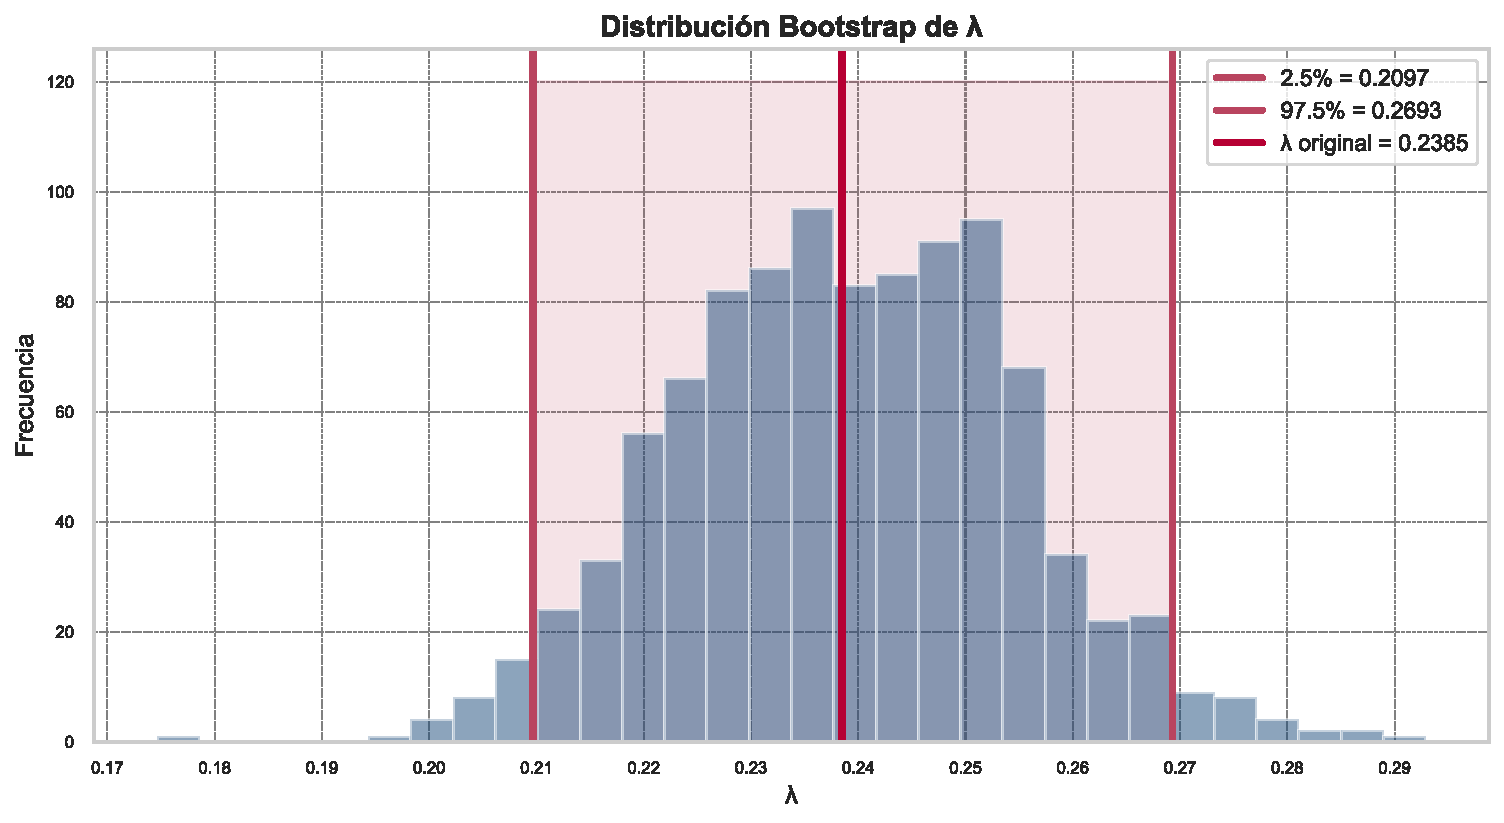
\includegraphics[width=0.75\textwidth]{imagenes/03-06-lambda-yj-bootstrapping.pdf}
    \caption{\textit{Elaboración Propia}. Distribución bootstrap del parámetro $\lambda$ para la transformación de Yeo-Johnson.}
\end{figure}


\subsubsection{Serie Transformada}
Una vez aplicada la transformación de Yeo-Johnson estandarizada a la serie original de precipitación mensual, se obtiene la siguiente representación gráfica en la Figura 10.

\begin{figure}[h!]
    \centering
    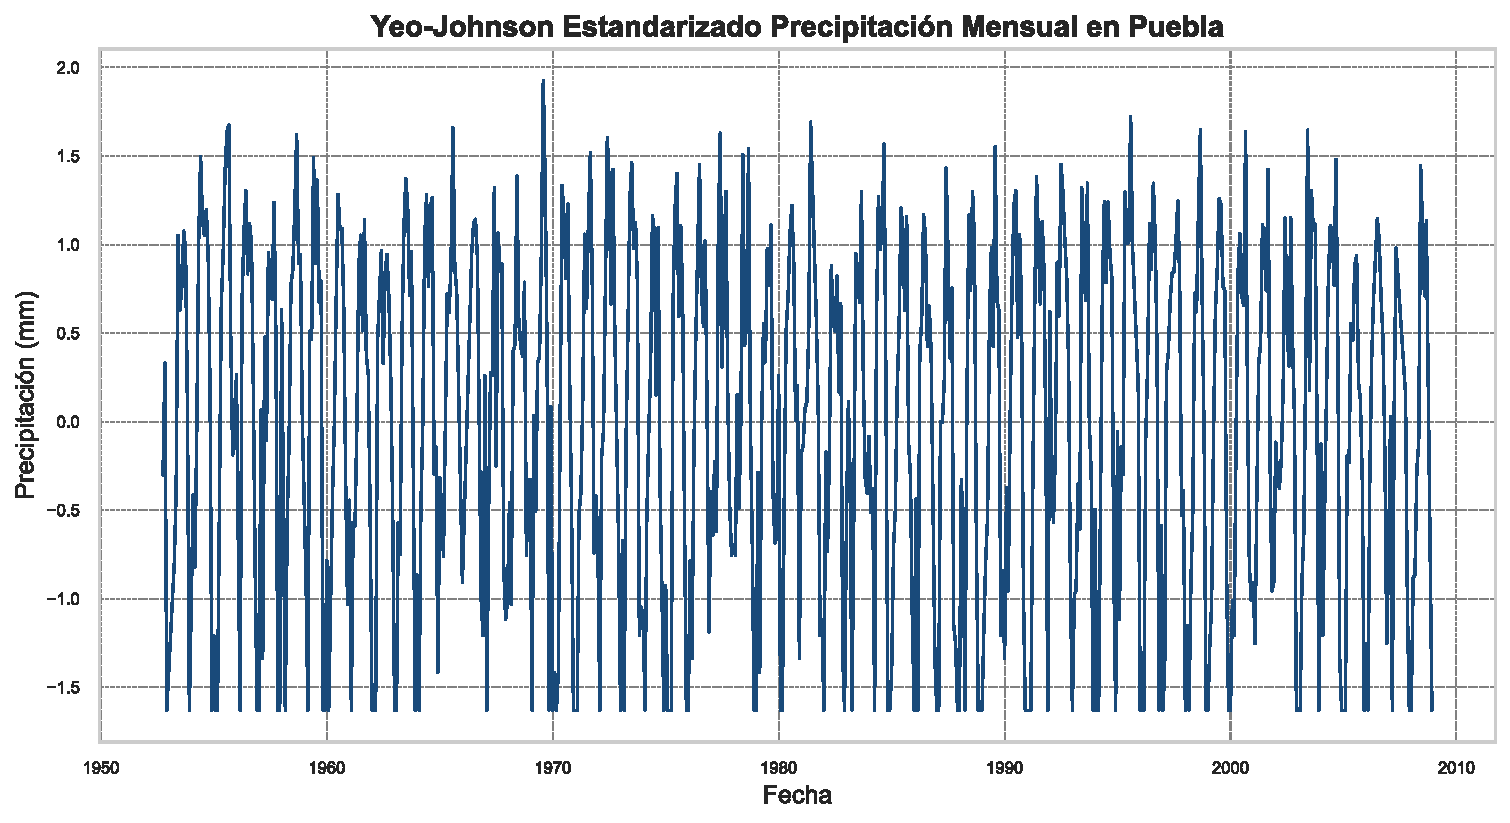
\includegraphics[width=0.8\textwidth]{imagenes/03-07-precipitacion_yeo_johnson.pdf}
    \caption{\textit{Elaboración Propia}. Serie de precipitación mensual en Puebla transformada con Yeo-Johnson y estandarizada.}
    \label{fig:yeojohnson_series}
\end{figure}



\textbf{Verificación de Estacionariedad de la Serie}

Para verificar la estacionariedad de la serie transformada con Yeo-Johnson, se aplicó la prueba de Dickey-Fuller aumentada (ADF). Los resultados fueron los siguientes:


\begin{itemize}
    \item Estadístico ADF: -6.885
    \item p-valor: $1.36 \times 10^{-9}$
    \item Valores críticos: -3.44 (1\%), -2.86 (5\%), -2.57 (10\%)
\end{itemize}


Dado que el estadístico ADF es menor que los valores críticos a todos los niveles y el p-valor es significativamente menor que $\alpha = 0.05$, se concluye que la serie transformada es estacionaria.

\vspace{0.5cm}
\newpage

\textbf{Autocorrelaciones Simples y Autocorrelaciones Parciales}

A continuación, se presentan las funciones de autocorrelación (FAC) y autocorrelación parcial (FACP) de la serie transformada de precipitación mensual:

\begin{figure}[h!]
    \centering
    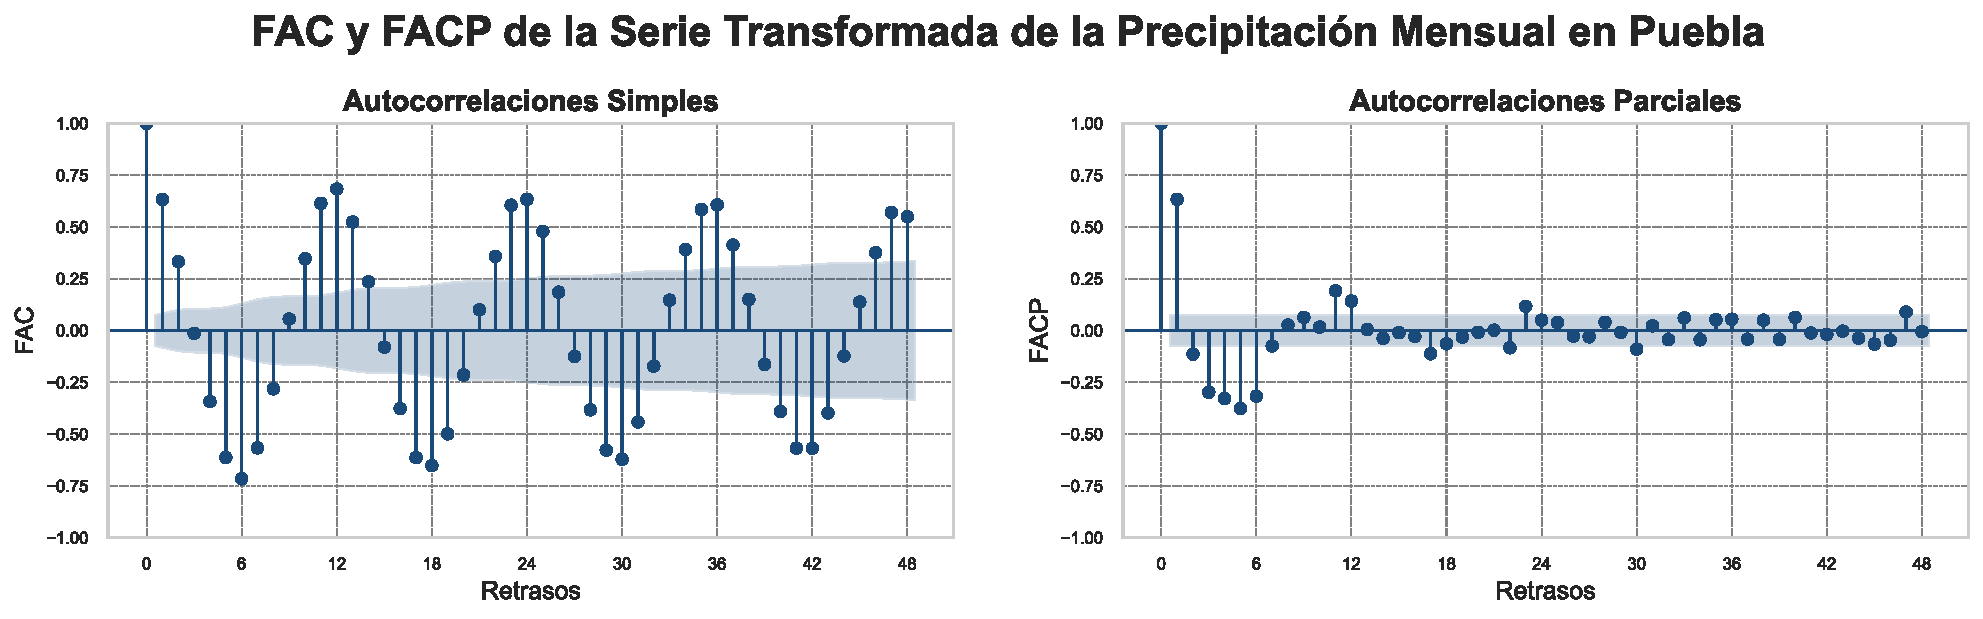
\includegraphics[width=0.9\textwidth]{imagenes/03-08-acf_pacf.pdf}
    \caption{\textit{Elaboración Propia}. FAC y FACP de la serie transformada (Yeo-Johnson) de precipitación mensual en Puebla.}
    \label{fig:FAC_FACP_yeo}
\end{figure}

También podemos notar un patrón estacional, igual que en el caso pasado, por lo que se aplicará la misma metodología, aplicar diferencias estacionales y comparar.




\newpage
\subsection{Diferencias Estacionales de la Serie con Transformación}

En esta sección se comparan las diferentes diferencias estacionales que se le pueden aplicar a la serie, con la que posteriormente entrenaremos al modelo.




  \subsubsection{Primera Diferencia Estacional}
  Los valores significativos de autocorrelación fueron los siguientes:

\begin{figure}[ht]
    \centering
    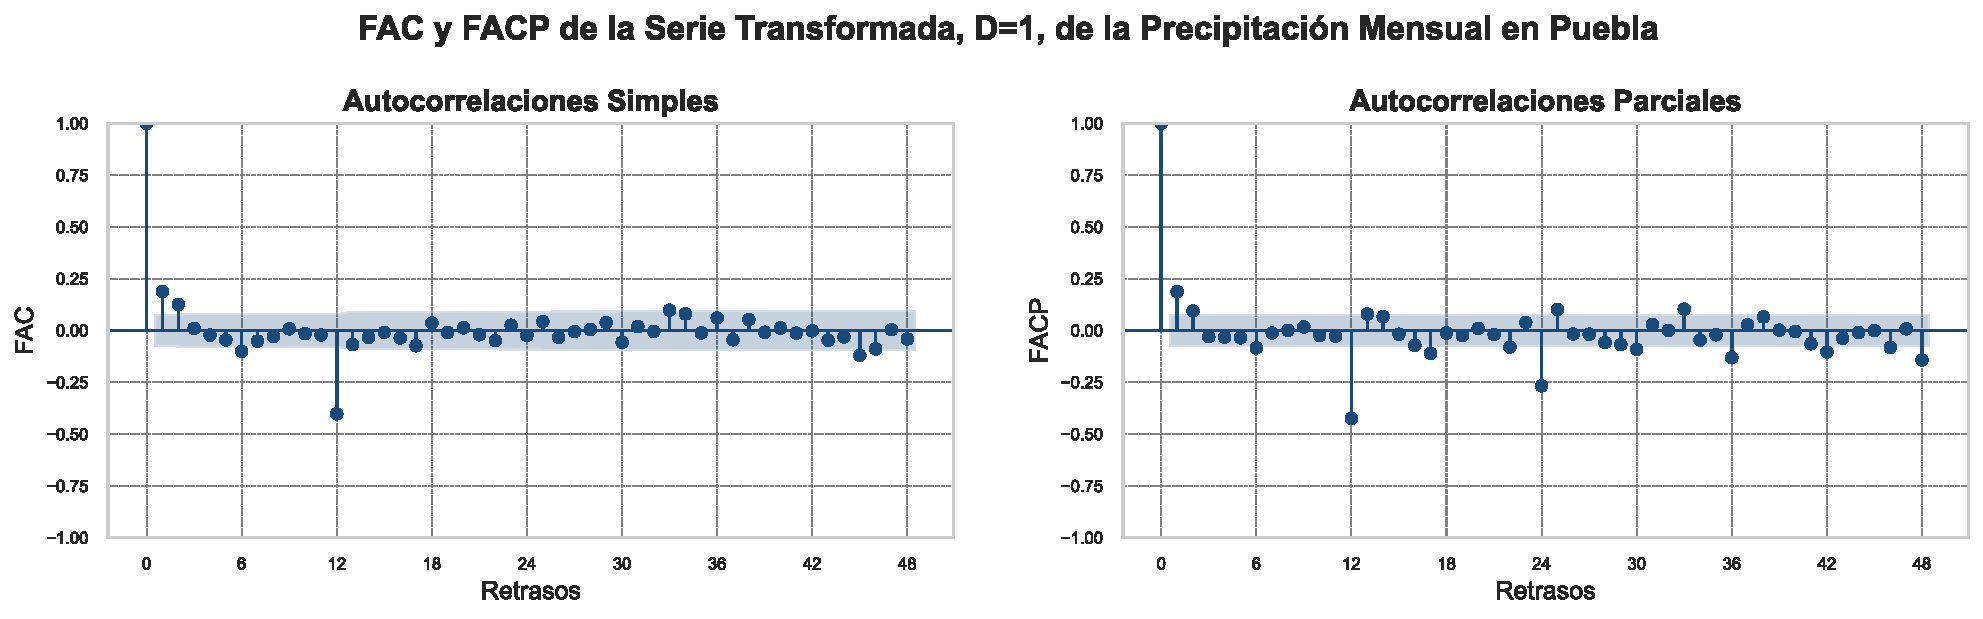
\includegraphics[width=0.8\textwidth]{imagenes/03-10-fac-facp-serie-D1.pdf}
    \caption{\textit{Elaboración Propia}. FAC y FACP de la Primera Diferencia Estacional}
\end{figure}


Los valores significativos de autocorrelación fueron los siguientes:
\begin{multicols}{5}
\scriptsize
\begin{itemize}
    \item $r_1$: 0.188
    \item $r_2$: 0.126
    \item $r_6$: -0.100
    \item $r_{12}$: -0.402
    \item $r_{33}$: 0.098
    \item $r_{45}$: -0.120
\end{itemize}
\end{multicols}

Los valores significativos de autocorrelación parcial fueron los siguientes:
\begin{multicols}{5}
\scriptsize
\begin{itemize}
    \item $\rho_1$: 0.188
    \item $\rho_2$: 0.094
    \item $\rho_6$: -0.085
    \item $\rho_{12}$: -0.432
    \item $\rho_{13}$: 0.081
    \item $\rho_{17}$: -0.114
    \item $\rho_{22}$: -0.084
    \item $\rho_{24}$: -0.281
    \item $\rho_{25}$: 0.108
    \item $\rho_{30}$: -0.097
    \item $\rho_{33}$: 0.111
    \item $\rho_{36}$: -0.146
    \item $\rho_{42}$: -0.118
    \item $\rho_{46}$: -0.094
    \item $\rho_{48}$: -0.167
    \item $\rho_{50}$: 0.092
    \item $\rho_{55}$: 0.093
    \item $\rho_{60}$: -0.100
    \item $\rho_{72}$: -0.130
    \item $\rho_{78}$: -0.080
    \item $\rho_{84}$: -0.080
    \item $\rho_{92}$: -0.140
    \item $\rho_{93}$: 0.116
    \item $\rho_{94}$: -0.122
    \item $\rho_{113}$: -0.086
    \item $\rho_{118}$: -0.082
    \item $\rho_{120}$: -0.116
\end{itemize}
\end{multicols}



\textbf{Verificar Estacionariedad en la Serie}



\begin{itemize}
    \item Estadístico ADF: -9.030
    \item p-valor: $5.46 \times 10^{-15}$
    \item Valores críticos: -3.44 (1\%), -2.87 (5\%), -2.57 (10\%)
\end{itemize}

El estadístico ADF es $-9.030$, valor muy por debajo de todos los umbrales críticos y el p-valor es $5.46 \times 10^{-15}$, muchísimo menor que cualquier nivel de significancia. Por lo que se rechaza la hipótesis nula, es decir, la serie es estacionaria.


















  \subsubsection{Segunda Diferencia Estacional}

Así se ve la FAC y la FACP de la segunda diferencia estacional de la serie transformada:
  \begin{figure}[ht]
    \centering
    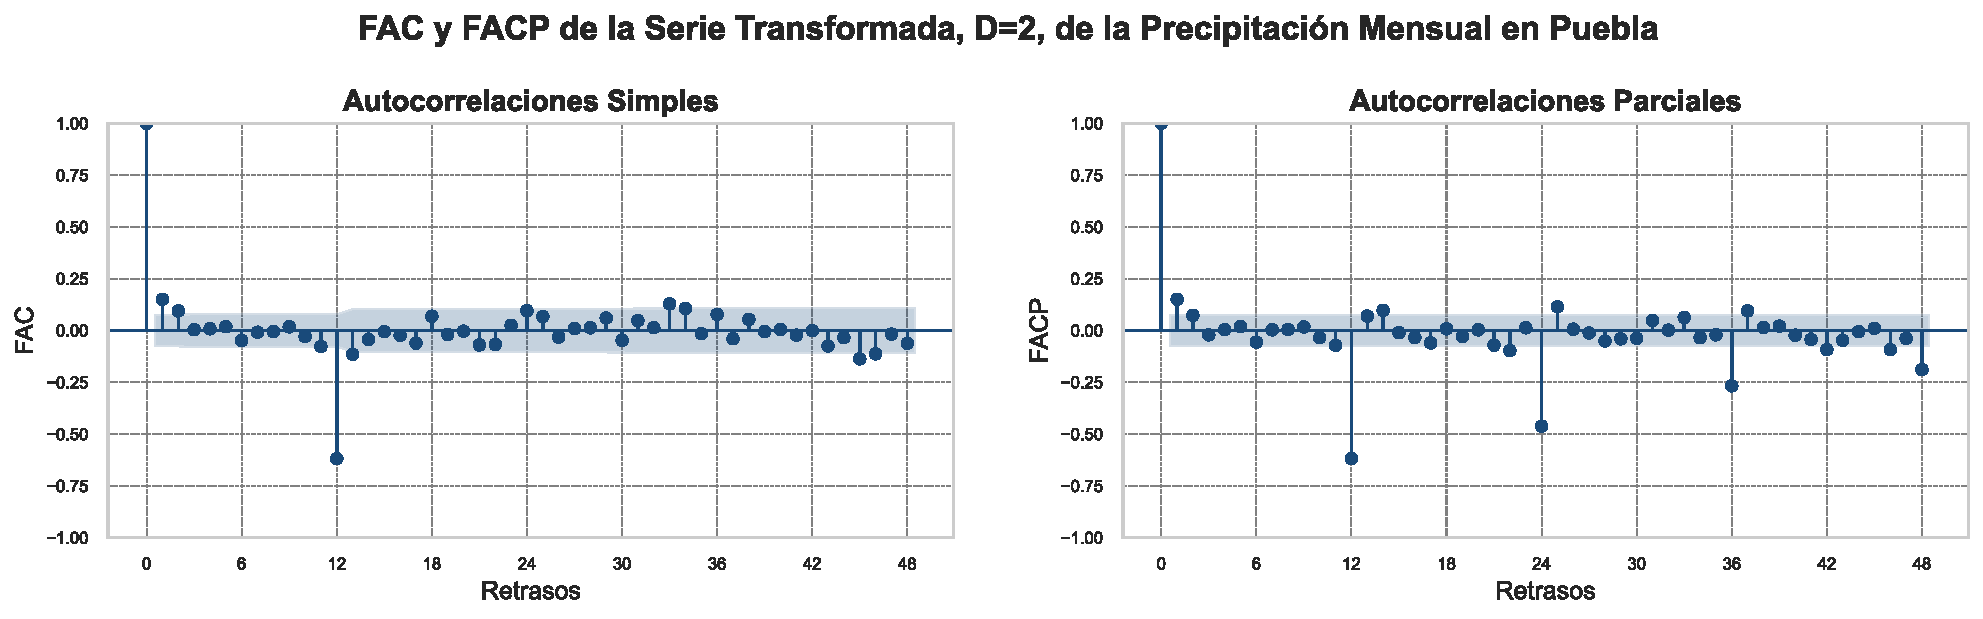
\includegraphics[width=0.8\textwidth]{imagenes/03-11-fac-facp-serie-D2.pdf}
    \caption{\textit{Elaboración Propia}. FAC y FACP de la Segunda Diferencia Estacional de la Serie Transformada}
\end{figure}


Los valores significativos de autocorrelación fueron los siguientes:
\begin{multicols}{5}
\scriptsize
\begin{itemize}
    \item $r_1$: 0.151
    \item $r_2$: 0.095
    \item $r_{12}$: -0.618
    \item $r_{13}$: -0.115
    \item $r_{33}$: 0.129
    \item $r_{45}$: -0.137
    \item $r_{46}$: -0.112
\end{itemize}
\end{multicols}

Los valores significativos de autocorrelación parcial fueron los siguientes:
\begin{multicols}{5}
\scriptsize
\begin{itemize}
    \item $\rho_1$: 0.151
    \item $\rho_{12}$: -0.630
    \item $\rho_{14}$: 0.102
    \item $\rho_{22}$: -0.103
    \item $\rho_{24}$: -0.493
    \item $\rho_{25}$: 0.127
    \item $\rho_{36}$: -0.317
    \item $\rho_{37}$: 0.123
    \item $\rho_{42}$: -0.117
    \item $\rho_{46}$: -0.120
    \item $\rho_{48}$: -0.270
    \item $\rho_{50}$: 0.082
    \item $\rho_{54}$: -0.121
    \item $\rho_{58}$: -0.097
    \item $\rho_{60}$: -0.172
    \item $\rho_{61}$: 0.127
    \item $\rho_{64}$: -0.084
    \item $\rho_{66}$: -0.133
    \item $\rho_{67}$: 0.108
    \item $\rho_{70}$: -0.182
    \item $\rho_{71}$: 0.154
    \item $\rho_{72}$: -0.284
    \item $\rho_{73}$: 0.288
    \item $\rho_{74}$: -0.265
    \item $\rho_{75}$: 0.276
    \item $\rho_{76}$: -0.498
    \item $\rho_{77}$: 0.946
    \item $\rho_{78}$: -19.481
    \item $\rho_{79}$: -1.053
    \item $\rho_{80}$: 0.617
    \item $\rho_{81}$: -0.368
    \item $\rho_{82}$: 0.198
    \item $\rho_{83}$: -0.110
    \item $\rho_{85}$: -0.144
    \item $\rho_{86}$: 0.254
    \item $\rho_{87}$: -0.193
    \item $\rho_{89}$: -0.081
    \item $\rho_{92}$: 0.125
    \item $\rho_{93}$: -0.104
    \item $\rho_{95}$: -0.089
    \item $\rho_{96}$: -0.083
    \item $\rho_{98}$: 0.205
    \item $\rho_{99}$: -0.194
    \item $\rho_{102}$: -0.129
    \item $\rho_{104}$: 0.191
    \item $\rho_{105}$: -0.293
    \item $\rho_{108}$: -0.188
    \item $\rho_{110}$: 0.309
    \item $\rho_{111}$: -0.513
    \item $\rho_{112}$: 0.092
    \item $\rho_{113}$: 0.376
    \item $\rho_{114}$: -0.795
    \item $\rho_{115}$: 1.170
    \item $\rho_{116}$: -5.319
    \item $\rho_{117}$: -2.444
    \item $\rho_{118}$: 1.410
    \item $\rho_{119}$: -0.889
    \item $\rho_{120}$: 0.451
\end{itemize}
\end{multicols}













  \subsubsection{Tercera Diferencia Estacional}

Así se ve la FAC y la FACP de la tercera diferencia estacional de la serie transformada:

\begin{figure}[ht]
    \centering
    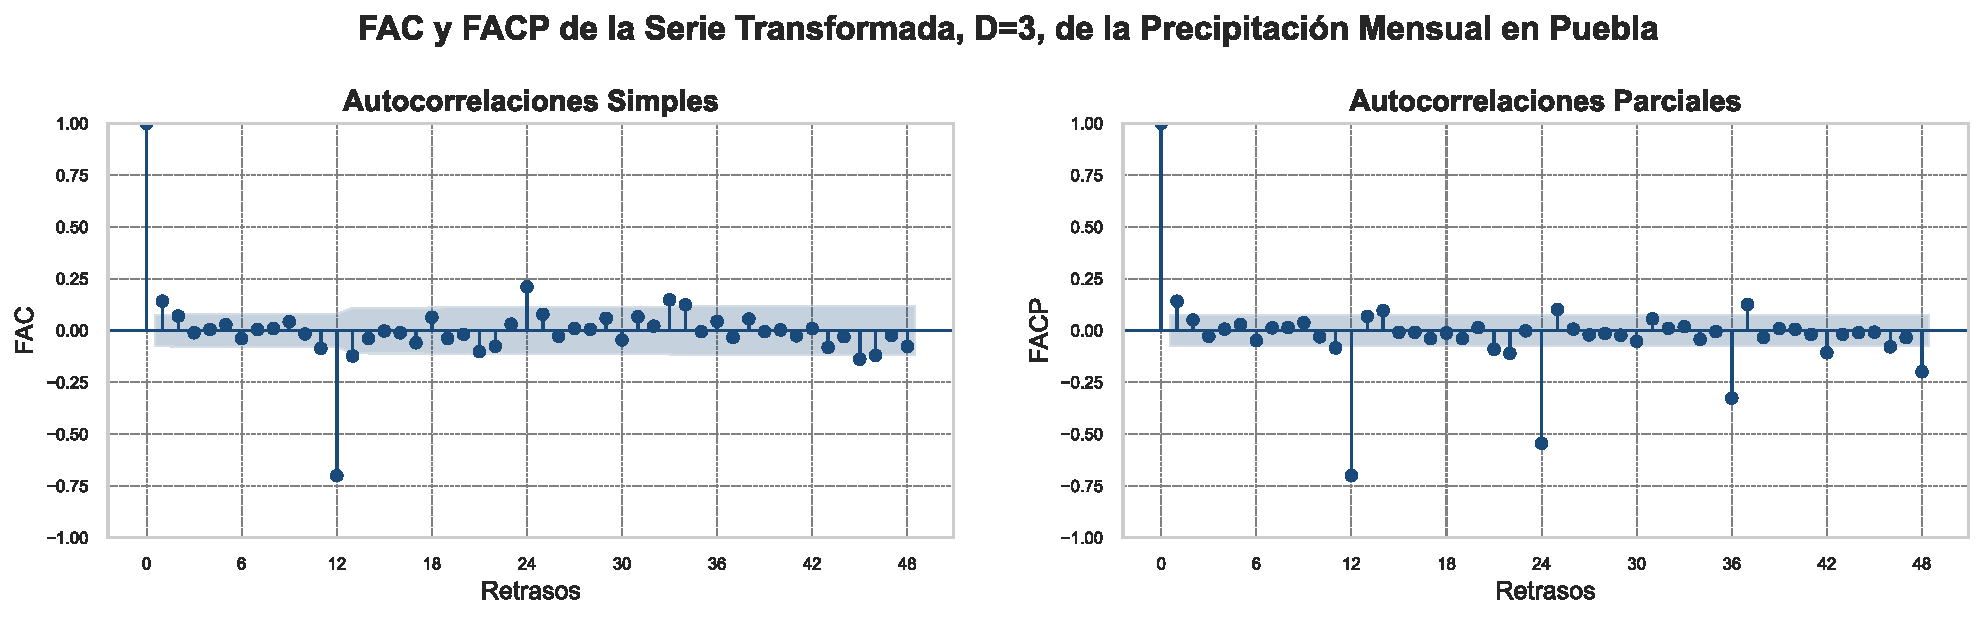
\includegraphics[width=0.8\textwidth]{imagenes/03-12-fac-facp-serie-D3.pdf}
    \caption{\textit{Elaboración Propia}. FAC y FACP de la Tercera Diferencia Estacional de la Serie Transformada}
\end{figure}

Los valores significativos de autocorrelación fueron los siguientes:
\begin{multicols}{5}
\scriptsize
\begin{itemize}
    \item $r_1$: 0.141
    \item $r_{11}$: -0.086
    \item $r_{12}$: -0.701
    \item $r_{13}$: -0.123
    \item $r_{24}$: 0.211
    \item $r_{33}$: 0.148
    \item $r_{34}$: 0.124
    \item $r_{45}$: -0.138
\end{itemize}
\end{multicols}

Los valores significativos de autocorrelación parcial fueron los siguientes:
\begin{multicols}{5}
\scriptsize
\begin{itemize}
    \item $\rho_1$: 0.142
    \item $\rho_{11}$: -0.086
    \item $\rho_{12}$: -0.715
    \item $\rho_{14}$: 0.102
    \item $\rho_{21}$: -0.097
    \item $\rho_{22}$: -0.120
    \item $\rho_{24}$: -0.591
    \item $\rho_{25}$: 0.116
    \item $\rho_{36}$: -0.426
    \item $\rho_{37}$: 0.187
    \item $\rho_{42}$: -0.173
    \item $\rho_{46}$: -0.113
    \item $\rho_{48}$: -0.397
    \item $\rho_{49}$: 0.174
    \item $\rho_{54}$: -0.327
    \item $\rho_{55}$: 0.216
    \item $\rho_{56}$: -0.195
    \item $\rho_{58}$: -0.223
    \item $\rho_{59}$: 0.252
    \item $\rho_{60}$: -0.738
    \item $\rho_{61}$: 2.254
    \item $\rho_{62}$: 1.650
    \item $\rho_{63}$: -0.697
    \item $\rho_{64}$: 0.397
    \item $\rho_{65}$: -0.212
    \item $\rho_{66}$: -0.205
    \item $\rho_{68}$: 0.236
    \item $\rho_{69}$: -0.819
    \item $\rho_{70}$: 1.301
    \item $\rho_{71}$: 1.432
    \item $\rho_{72}$: -5.899
    \item $\rho_{73}$: -1.320
    \item $\rho_{74}$: -0.677
    \item $\rho_{75}$: 0.525
    \item $\rho_{76}$: -0.282
    \item $\rho_{77}$: -0.452
    \item $\rho_{78}$: 0.301
    \item $\rho_{79}$: -0.416
    \item $\rho_{80}$: -0.119
    \item $\rho_{81}$: -0.154
    \item $\rho_{82}$: -0.292
    \item $\rho_{83}$: -0.493
    \item $\rho_{84}$: -0.150
    \item $\rho_{85}$: -0.893
    \item $\rho_{86}$: -5.929
    \item $\rho_{87}$: 1.212
    \item $\rho_{88}$: 0.515
    \item $\rho_{89}$: 0.246
    \item $\rho_{90}$: 0.528
    \item $\rho_{92}$: 0.331
    \item $\rho_{93}$: 0.115
    \item $\rho_{94}$: 0.212
    \item $\rho_{95}$: -0.129
    \item $\rho_{96}$: 0.514
    \item $\rho_{97}$: -0.619
    \item $\rho_{98}$: 1.710
    \item $\rho_{99}$: 2.121
    \item $\rho_{100}$: -0.606
    \item $\rho_{101}$: 0.461
    \item $\rho_{102}$: -0.157
    \item $\rho_{103}$: 0.254
    \item $\rho_{104}$: -0.210
    \item $\rho_{105}$: 0.313
    \item $\rho_{107}$: 0.121
    \item $\rho_{109}$: 0.104
    \item $\rho_{110}$: -0.172
    \item $\rho_{111}$: 0.265
    \item $\rho_{112}$: -0.116
    \item $\rho_{114}$: 0.185
    \item $\rho_{115}$: 0.108
    \item $\rho_{116}$: -0.159
    \item $\rho_{117}$: 0.378
    \item $\rho_{118}$: -0.124
    \item $\rho_{120}$: 0.206
\end{itemize}
\end{multicols}



\newpage
  \subsubsection{Comparación de Desviaciones Estándar con Distintas Diferencias}

\begin{figure}[ht]
    \centering
    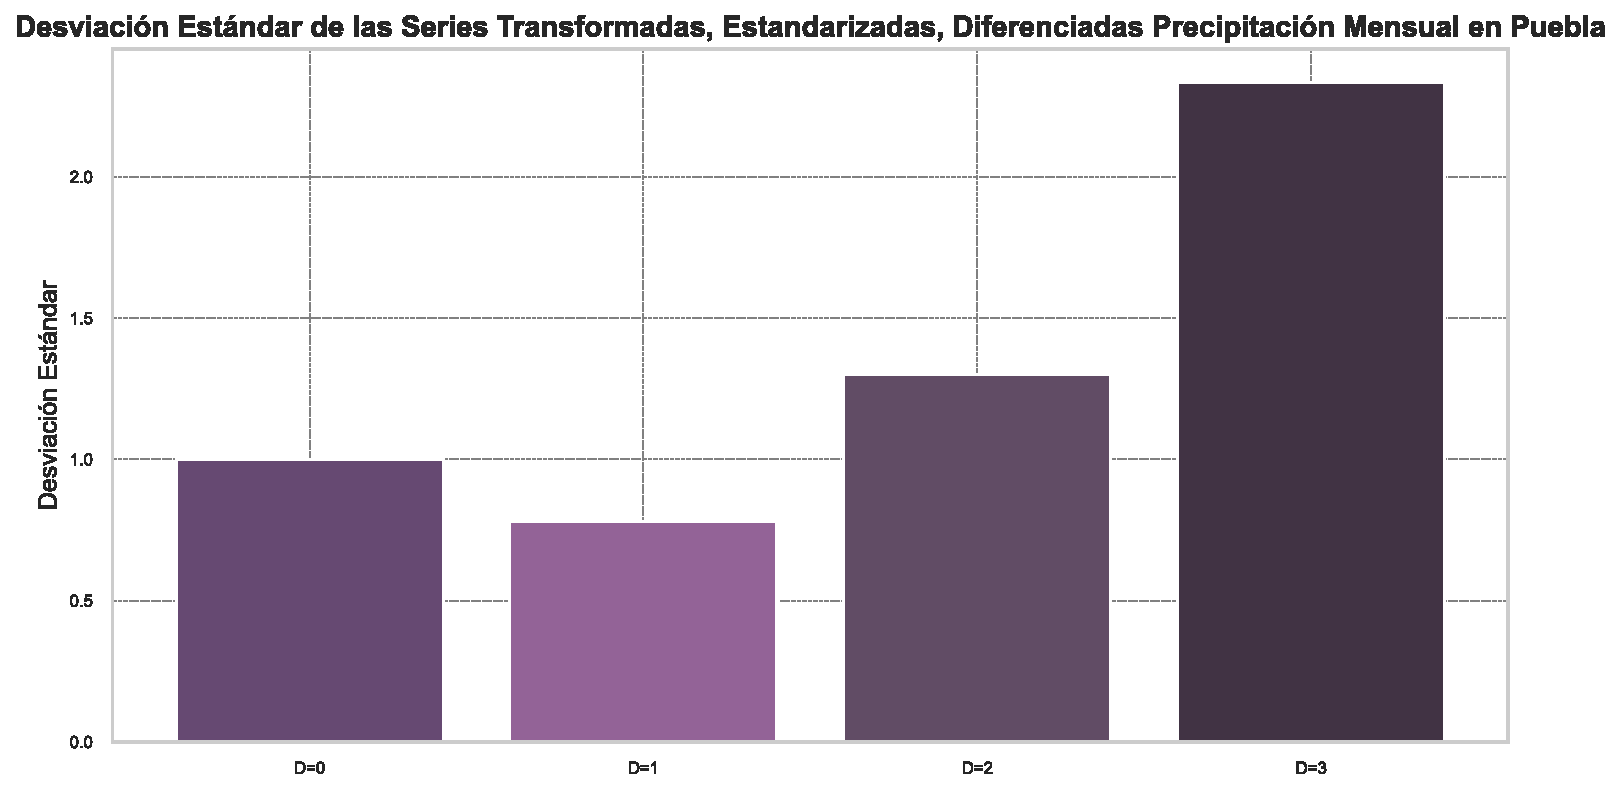
\includegraphics[width=0.8\textwidth]{imagenes/03-13-std-Ds.pdf}
    \caption{\textit{Elaboración Propia}. Desviación estándar de la serie transformada y estandarizada, con diferencias estacionales de primer, segundo y tercer orden.}
\end{figure}

Ocurre lo mismo que en las diferencias de la serie sin transformaciones,  
Tal como se observó en el caso de las diferencias aplicadas a la serie original sin transformaciones, el comportamiento de la desviación estándar se ve afectado por el orden de la diferencia estacional. Se observa que la menor varianza corresponde a la serie con una primera diferencia estacional. En consecuencia, se decide conservar únicamente la primera diferencia estacional. Es interesante notar que con la transformación y las diferencias, las autocorrelaciones parciales simples aumentan notablemente en cantidad, a comparación de las autocorrelaciones parciales de la serie sin transformación,  tal vez la transformación no era la adecuada para el objetivo de modelado.


\newpage
\subsection{Modelado}

En esta sección se muestra el proceso de modelado para la serie transformada y para la serie sin transformar.

\subsubsection{Serie sin Transformaciones}

Para la serie sin transformaciones, se hizo un modelado donde se realizaron 252 modelos con diferentes hiperparámetros y se seleccionaba el modelo que tenía el menor AIC.

Primero se intentó con la librería pmdarima, que realiza distintas combinaciones hasta orden dos, obteniendo estos resultados:
\begin{smallconsole}[caption={Modelos con pmdarima}]
(1)  ARIMA(1,0,0)(0,1,1)[12], AIC=1430.397
(2)  ARIMA(0,0,1)(0,1,1)[12], AIC=1431.266
(3)  ARIMA(1,0,1)(0,1,1)[12], AIC=1432.133
(4)  ARIMA(2,0,0)(0,1,1)[12], AIC=1432.157
(5)  ARIMA(1,0,0)(0,1,2)[12], AIC=1432.368
(6)  ARIMA(1,0,0)(1,1,1)[12], AIC=1432.373
(7)  ARIMA(0,0,2)(0,1,1)[12], AIC=1432.664
(8)  ARIMA(0,0,1)(0,1,2)[12], AIC=1433.240
(9)  ARIMA(0,0,1)(1,1,1)[12], AIC=1433.245
(10) ARIMA(2,0,1)(0,1,1)[12], AIC=1434.127
(11) ARIMA(0,0,0)(0,1,1)[12], AIC=1445.334
(12) ARIMA(1,0,0)(1,1,0)[12], AIC=1523.141
(13) ARIMA(0,0,1)(1,1,0)[12], AIC=1523.219
(14) ARIMA(0,0,1)(0,1,0)[12], AIC=1652.849
(15) ARIMA(1,0,0)(0,1,0)[12], AIC=1652.984
(16) ARIMA(0,0,0)(0,1,0)[12], AIC=1655.671
\end{smallconsole}

Sin embargo, ninguno cumplió los supuestos en los residuos, por lo que se decidió no usar la librería e ir a ordenes mayores. También, para poder visualizar los resultados en base a su AIC, se fueron variando dos hiperparámetros, es decir, entre $p, q, P, Q$, dos se fijaban con un valor de cero, y se calculaba el AIC para distintos modelos recorriendo los valores que no estaban fijos. Es decir:

- Se fijan los valores de $\text{ARIMA}(p, 0, q) \times (0, 1, 0, 12)$ donde $p = 0, 1, 2, \dots$ y $q = 0, 1, 2, \dots$.  

- Se fijan los valores de $\text{ARIMA}(0, 0, q) \times (P, 1, 0, 12)$ donde $P = 0, 1, 2, \dots$ y $q = 0, 1, 2, \dots$.  

- Se fijan los valores de $\text{ARIMA}(p, 0, 0) \times (0, 1, Q, 12)$ donde $p = 0, 1, 2, \dots$ y $Q = 0, 1, 2, \dots$.  

- Se fijan los valores de $\text{ARIMA}(0, 0, 0) \times (P, 1, Q, 12)$ donde $P = 0, 1, 2, \dots$ y $Q = 0, 1, 2, \dots$.



\newpage
Se fijan los valores de $\text{ARIMA}(p, 0, q) \times (0, 1, 0, 12)$ donde $p = 0, 1, 2, \dots$ y $q = 0, 1, 2, \dots$.

\begin{figure}[h!]
    \centering
    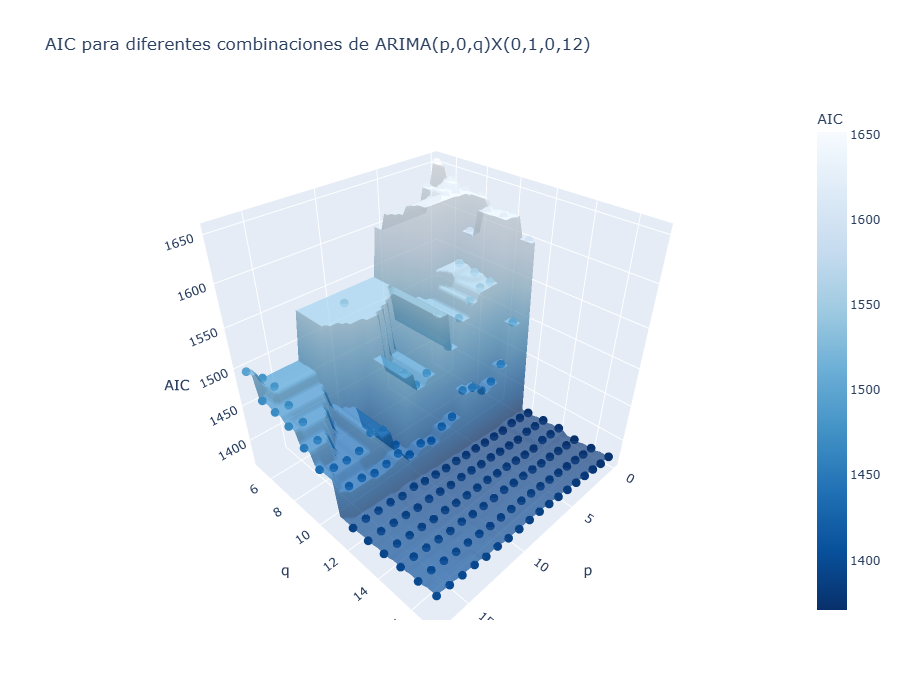
\includegraphics[width=0.9\textwidth]{imagenes/99-01.png}
    \caption{\textit{Elaboración Propia}. AIC donde $p = 0, 1, 2, \dots$ y $q = 0, 1, 2, \dots$.}
    \label{fig:FAC_FACP_yeo}
\end{figure}

\begin{smallconsole}[caption={donde $p = 0, 1, 2, \dots$ y $q = 0, 1, 2, \dots$.}]
(1) ARIMA(12,0,0)(0,1,4)[12], AIC=1367.04
(2) ARIMA(13,0,0)(0,1,4)[12], AIC=1367.37
(3) ARIMA(12,0,0)(0,1,3)[12], AIC=1368.24
(4) ARIMA(12,0,0)(0,1,5)[12], AIC=1369.25
(5) ARIMA(0,0,15)(0,1,0)[12], AIC=1370.81
(6) ARIMA(0,0,15)(0,1,0)[12], AIC=1370.81
(7) ARIMA(0,0,12)(0,1,0)[12], AIC=1370.92
(8) ARIMA(0,0,12)(0,1,0)[12], AIC=1370.92
(9) ARIMA(15,0,0)(0,1,4)[12], AIC=1371.49
(10) ARIMA(3,0,12)(0,1,0)[12], AIC=1372.25
(11) ARIMA(0,0,16)(0,1,0)[12], AIC=1372.52
(12) ARIMA(1,0,15)(0,1,0)[12], AIC=1372.60
(13) ARIMA(1,0,12)(0,1,0)[12], AIC=1372.69
(14) ARIMA(0,0,13)(0,1,0)[12], AIC=1372.78
(15) ARIMA(0,0,12)(1,1,0)[12], AIC=1372.79
\end{smallconsole}

Parece que no hay una gran diferencia entre modelos luego de que $q$, la parte media móvil, es mayor a $12$, siendo el mejor modelo un ARIMA(12,0,0)(0,1,4)[12], con un AIC=1367.04.

\newpage
Se fijan los valores de $\text{ARIMA}(0, 0, q) \times (P, 1, 0, 12)$ donde $P = 0, 1, 2, \dots$ y $q = 0, 1, 2, \dots$.
\begin{figure}[h!]
    \centering
    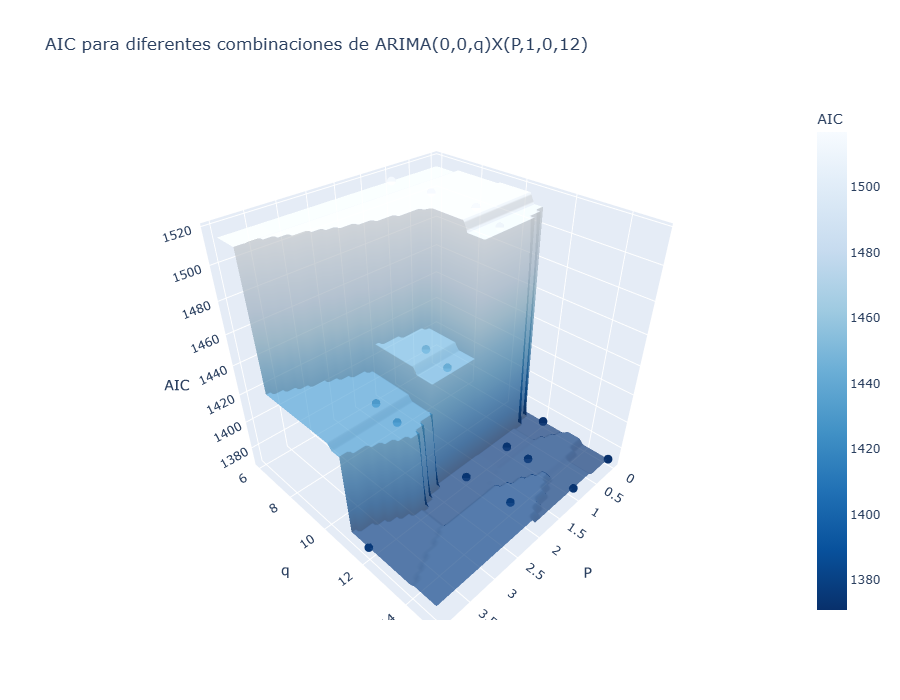
\includegraphics[width=0.9\textwidth]{imagenes/99-02.png}
    \caption{\textit{Elaboración Propia}. AIC donde $q = 0, 1, 2, \dots$ y $P = 0, 1, 2, \dots$.}
    \label{fig:FAC_FACP_yeo}
\end{figure}

\begin{smallconsole}[caption={donde $q = 0, 1, 2, \dots$ y $P = 0, 1, 2, \dots$.}]
(1) ARIMA(12,0,0)(0,1,4)[12], AIC=1367.04
(2) ARIMA(13,0,0)(0,1,4)[12], AIC=1367.37
(3) ARIMA(12,0,0)(0,1,3)[12], AIC=1368.24
(4) ARIMA(12,0,0)(0,1,5)[12], AIC=1369.25
(5) ARIMA(0,0,15)(0,1,0)[12], AIC=1370.81
(6) ARIMA(0,0,15)(0,1,0)[12], AIC=1370.81
(7) ARIMA(0,0,12)(0,1,0)[12], AIC=1370.92
(8) ARIMA(0,0,12)(0,1,0)[12], AIC=1370.92
(9) ARIMA(15,0,0)(0,1,4)[12], AIC=1371.49
(10) ARIMA(3,0,12)(0,1,0)[12], AIC=1372.25
(11) ARIMA(0,0,16)(0,1,0)[12], AIC=1372.52
(12) ARIMA(1,0,15)(0,1,0)[12], AIC=1372.60
(13) ARIMA(1,0,12)(0,1,0)[12], AIC=1372.69
(14) ARIMA(0,0,13)(0,1,0)[12], AIC=1372.78
(15) ARIMA(0,0,12)(1,1,0)[12], AIC=1372.79
\end{smallconsole}

Por el costo computacional, en esta y las siguientes no se realiza una comparación tan granulada, sino que se van dando saltos, suponiendo que el AIC es parecido por zonas, se volvió a llegar al mismo resultado que en el anterior con un ARIMA(12,0,0)(0,1,4)[12], que cuenta con un AIC de 1367.04.

\newpage
Se fijan los valores de $\text{ARIMA}(p, 0, 0) \times (0, 1, Q, 12)$ donde $p = 0, 1, 2, \dots$ y $Q = 0, 1, 2, \dots$.
\begin{figure}[h!]
    \centering
    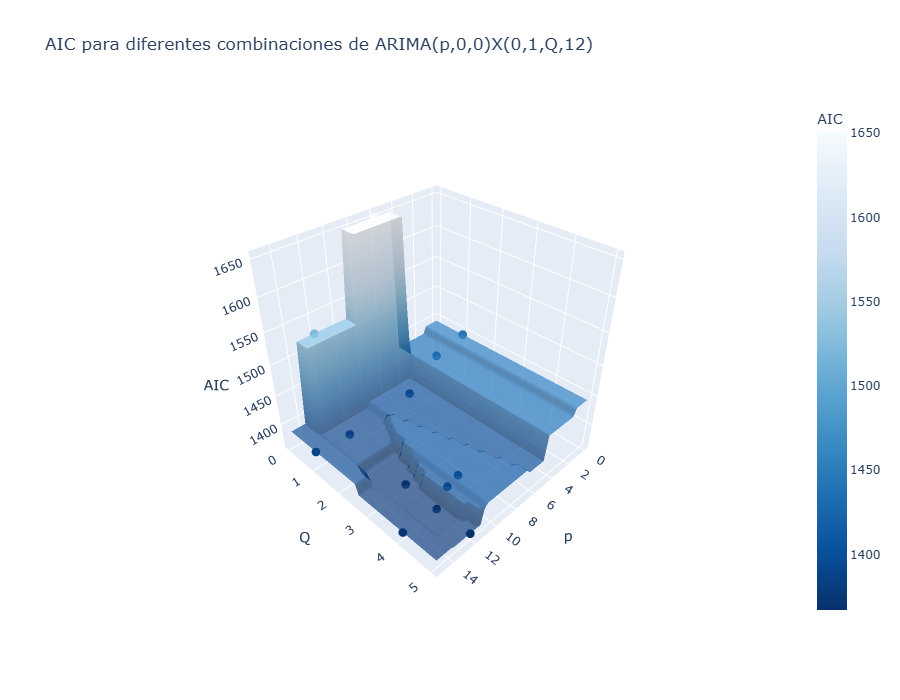
\includegraphics[width=0.9\textwidth]{imagenes/99-03.png}
    \caption{\textit{Elaboración Propia}. AIC donde $p = 0, 1, 2, \dots$ y $Q = 0, 1, 2, \dots$.}
    \label{fig:FAC_FACP_yeo}
\end{figure}

\begin{smallconsole}[caption={donde $p = 0, 1, 2, \dots$ y $Q = 0, 1, 2, \dots$.}]
(1) ARIMA(12,0,0)(0,1,4)[12], AIC=1367.04
(2) ARIMA(13,0,0)(0,1,4)[12], AIC=1367.37
(3) ARIMA(12,0,0)(0,1,3)[12], AIC=1368.24
(4) ARIMA(12,0,0)(0,1,5)[12], AIC=1369.25
(5) ARIMA(0,0,15)(0,1,0)[12], AIC=1370.81
(6) ARIMA(0,0,15)(0,1,0)[12], AIC=1370.81
(7) ARIMA(0,0,12)(0,1,0)[12], AIC=1370.92
(8) ARIMA(0,0,12)(0,1,0)[12], AIC=1370.92
(9) ARIMA(15,0,0)(0,1,4)[12], AIC=1371.49
(10) ARIMA(3,0,12)(0,1,0)[12], AIC=1372.25
(11) ARIMA(0,0,16)(0,1,0)[12], AIC=1372.52
(12) ARIMA(1,0,15)(0,1,0)[12], AIC=1372.60
(13) ARIMA(1,0,12)(0,1,0)[12], AIC=1372.69
(14) ARIMA(0,0,13)(0,1,0)[12], AIC=1372.78
(15) ARIMA(0,0,12)(1,1,0)[12], AIC=1372.79
\end{smallconsole}
Se puede observar un valle en el mejor ARIMA que tenemos, ARIMA(12,0,0)(0,1,4)[12], AIC=1367.04, se compararon con sus 4 puntos mas cercanos para confirmar que este punto puede ser visto como un mínimo, en cuanto a AIC se refiere.
\newpage
Se fijan los valores de $\text{ARIMA}(0, 0, 0) \times (P, 1, Q, 12)$ donde $P = 0, 1, 2, \dots$ y $Q = 0, 1, 2, \dots$.
\begin{figure}[h!]
    \centering
    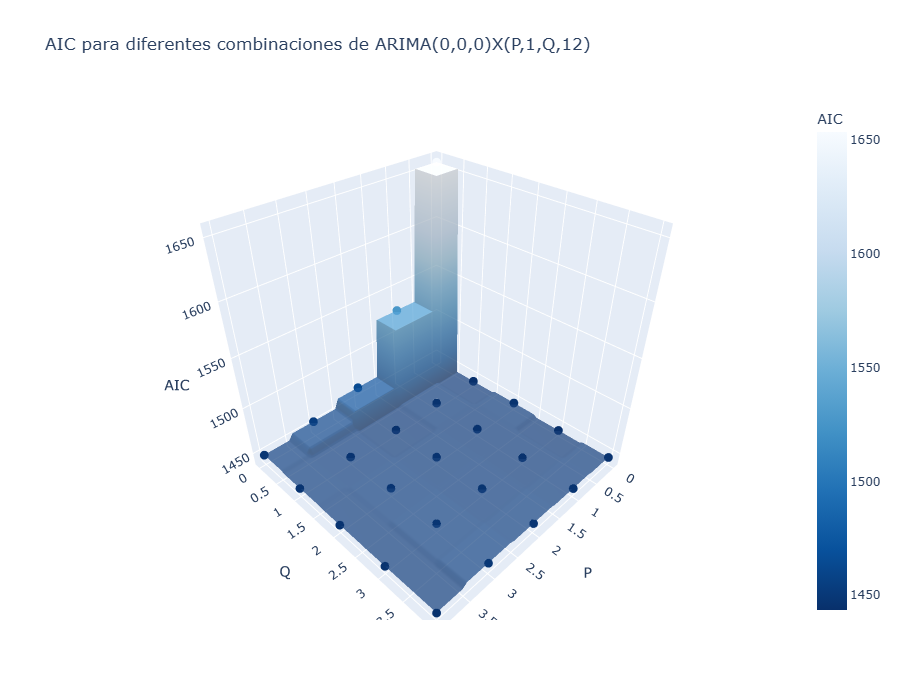
\includegraphics[width=0.9\textwidth]{imagenes/99-04.png}
    \caption{\textit{Elaboración Propia}. AIC donde $P = 0, 1, 2, \dots$ y $Q = 0, 1, 2, \dots$.}
    \label{fig:FAC_FACP_yeo}
\end{figure}

\begin{smallconsole}[caption={Modelos Ordenados por AIC donde $P = 0, 1, 2, \dots$ y $Q = 0, 1, 2, \dots$.}]
(1)   ARIMA(0,0,0)(0,1,3)[12]     AIC=1443.50  
(2)   ARIMA(0,0,0)(0,1,1)[12]     AIC=1443.59  
(3)   ARIMA(0,0,0)(2,1,1)[12]     AIC=1444.11  
(4)   ARIMA(0,0,0)(1,1,2)[12]     AIC=1445.15  
(5)   ARIMA(0,0,0)(1,1,3)[12]     AIC=1445.28  
(6)   ARIMA(0,0,0)(0,1,4)[12]     AIC=1445.49  
(7)   ARIMA(0,0,0)(0,1,2)[12]     AIC=1445.59  
(8)   ARIMA(0,0,0)(1,1,1)[12]     AIC=1445.59  
(9)   ARIMA(0,0,0)(4,1,3)[12]     AIC=1445.70  
(10)  ARIMA(0,0,0)(4,1,4)[12]     AIC=1445.74  
(11)  ARIMA(0,0,0)(2,1,2)[12]     AIC=1445.92  
(12)  ARIMA(0,0,0)(4,1,2)[12]     AIC=1445.95  
(13)  ARIMA(0,0,0)(3,1,1)[12]     AIC=1446.07  
(14)  ARIMA(0,0,0)(2,1,3)[12]     AIC=1446.38  
(15)  ARIMA(0,0,0)(1,1,4)[12]     AIC=1446.57  
(16)  ARIMA(0,0,0)(4,1,1)[12]     AIC=1446.70  
(17)  ARIMA(0,0,0)(3,1,2)[12]     AIC=1446.99  
\end{smallconsole}

Se puede observar que cuando se varía $P$ y $Q$, mientras se mantienen fijos $p=q=0$, se obtienen los modelos con menor AIC, mostrando la importancia de incluir partes no estacionales en el modelo.

\newpage

A continuación se muestran los resultados completos: 

\begin{smallconsole}[caption={Modelos Ordenados por AIC}]
(1) ARIMA(12,0,0)(0,1,4)[12], AIC=1367.04
(2) ARIMA(13,0,0)(0,1,4)[12], AIC=1367.37
(3) ARIMA(12,0,0)(0,1,3)[12], AIC=1368.24
(4) ARIMA(12,0,0)(0,1,5)[12], AIC=1369.25
(5) ARIMA(0,0,15)(0,1,0)[12], AIC=1370.81
(6) ARIMA(0,0,15)(0,1,0)[12], AIC=1370.81
(7) ARIMA(0,0,12)(0,1,0)[12], AIC=1370.92
(8) ARIMA(0,0,12)(0,1,0)[12], AIC=1370.92
(9) ARIMA(15,0,0)(0,1,4)[12], AIC=1371.49
(10) ARIMA(3,0,12)(0,1,0)[12], AIC=1372.25
(11) ARIMA(0,0,16)(0,1,0)[12], AIC=1372.52
(12) ARIMA(1,0,15)(0,1,0)[12], AIC=1372.60
(13) ARIMA(1,0,12)(0,1,0)[12], AIC=1372.69
(14) ARIMA(0,0,13)(0,1,0)[12], AIC=1372.78
(15) ARIMA(0,0,12)(1,1,0)[12], AIC=1372.79
(16) ARIMA(3,0,13)(0,1,0)[12], AIC=1372.87
(17) ARIMA(0,0,15)(1,1,0)[12], AIC=1373.17
(18) ARIMA(0,0,12)(2,1,0)[12], AIC=1373.37
(19) ARIMA(4,0,12)(0,1,0)[12], AIC=1373.41
(20) ARIMA(1,0,16)(0,1,0)[12], AIC=1373.59
(21) ARIMA(1,0,13)(0,1,0)[12], AIC=1373.76
(22) ARIMA(0,0,13)(1,1,0)[12], AIC=1373.86
(23) ARIMA(3,0,14)(0,1,0)[12], AIC=1374.01
(24) ARIMA(4,0,13)(0,1,0)[12], AIC=1374.12
(25) ARIMA(5,0,12)(0,1,0)[12], AIC=1374.34
(26) ARIMA(0,0,14)(0,1,0)[12], AIC=1374.44
(27) ARIMA(2,0,12)(0,1,0)[12], AIC=1374.49
(28) ARIMA(2,0,12)(0,1,0)[12], AIC=1374.49
(29) ARIMA(0,0,17)(0,1,0)[12], AIC=1374.49
(30) ARIMA(2,0,15)(0,1,0)[12], AIC=1374.62
(31) ARIMA(2,0,15)(0,1,0)[12], AIC=1374.62
(32) ARIMA(1,0,17)(0,1,0)[12], AIC=1374.97
(33) ARIMA(4,0,14)(0,1,0)[12], AIC=1375.08
(34) ARIMA(2,0,13)(0,1,0)[12], AIC=1375.16
(35) ARIMA(2,0,13)(0,1,0)[12], AIC=1375.16
(36) ARIMA(1,0,14)(0,1,0)[12], AIC=1375.26
(37) ARIMA(5,0,13)(0,1,0)[12], AIC=1375.43
(38) ARIMA(0,0,12)(4,1,0)[12], AIC=1375.93
(39) ARIMA(6,0,12)(0,1,0)[12], AIC=1375.94
(40) ARIMA(6,0,12)(0,1,0)[12], AIC=1375.94
(41) ARIMA(2,0,16)(0,1,0)[12], AIC=1375.97
(42) ARIMA(2,0,16)(0,1,0)[12], AIC=1375.97
(43) ARIMA(3,0,15)(0,1,0)[12], AIC=1376.37
(44) ARIMA(7,0,12)(0,1,0)[12], AIC=1376.46
(45) ARIMA(2,0,14)(0,1,0)[12], AIC=1376.63
(46) ARIMA(2,0,14)(0,1,0)[12], AIC=1376.63
(47) ARIMA(5,0,14)(0,1,0)[12], AIC=1377.04
(48) ARIMA(0,0,14)(2,1,0)[12], AIC=1377.49
(49) ARIMA(6,0,13)(0,1,0)[12], AIC=1377.52
(50) ARIMA(6,0,13)(0,1,0)[12], AIC=1377.52
(51) ARIMA(4,0,15)(0,1,0)[12], AIC=1377.61
(52) ARIMA(2,0,17)(0,1,0)[12], AIC=1377.67
(53) ARIMA(2,0,17)(0,1,0)[12], AIC=1377.67
(54) ARIMA(3,0,16)(0,1,0)[12], AIC=1377.71
(55) ARIMA(7,0,13)(0,1,0)[12], AIC=1378.15
(56) ARIMA(8,0,12)(0,1,0)[12], AIC=1378.47
(57) ARIMA(8,0,12)(0,1,0)[12], AIC=1378.47
(58) ARIMA(9,0,12)(0,1,0)[12], AIC=1378.79
(59) ARIMA(6,0,14)(0,1,0)[12], AIC=1378.97
(60) ARIMA(6,0,14)(0,1,0)[12], AIC=1378.97
(61) ARIMA(4,0,16)(0,1,0)[12], AIC=1379.46
(62) ARIMA(3,0,17)(0,1,0)[12], AIC=1379.51
(63) ARIMA(5,0,15)(0,1,0)[12], AIC=1379.68
(64) ARIMA(8,0,13)(0,1,0)[12], AIC=1380.15
(65) ARIMA(8,0,13)(0,1,0)[12], AIC=1380.15
(66) ARIMA(7,0,14)(0,1,0)[12], AIC=1380.53
(67) ARIMA(10,0,12)(0,1,0)[12], AIC=1380.62
(68) ARIMA(5,0,16)(0,1,0)[12], AIC=1380.90
(69) ARIMA(4,0,17)(0,1,0)[12], AIC=1381.04
(70) ARIMA(6,0,15)(0,1,0)[12], AIC=1381.49
(71) ARIMA(6,0,15)(0,1,0)[12], AIC=1381.49
(72) ARIMA(10,0,13)(0,1,0)[12], AIC=1381.66
(73) ARIMA(9,0,13)(0,1,0)[12], AIC=1381.75
(74) ARIMA(8,0,14)(0,1,0)[12], AIC=1382.31
(75) ARIMA(8,0,14)(0,1,0)[12], AIC=1382.31
(76) ARIMA(5,0,17)(0,1,0)[12], AIC=1382.35
(77) ARIMA(11,0,12)(0,1,0)[12], AIC=1382.48
(78) ARIMA(9,0,14)(0,1,0)[12], AIC=1382.58
(79) ARIMA(6,0,16)(0,1,0)[12], AIC=1382.64
(80) ARIMA(6,0,16)(0,1,0)[12], AIC=1382.64
(81) ARIMA(12,0,0)(0,1,1)[12], AIC=1382.66
(82) ARIMA(7,0,15)(0,1,0)[12], AIC=1382.73
(83) ARIMA(10,0,14)(0,1,0)[12], AIC=1383.53
(84) ARIMA(11,0,13)(0,1,0)[12], AIC=1383.82
(85) ARIMA(6,0,17)(0,1,0)[12], AIC=1384.31
(86) ARIMA(6,0,17)(0,1,0)[12], AIC=1384.31
(87) ARIMA(7,0,16)(0,1,0)[12], AIC=1384.33
(88) ARIMA(8,0,15)(0,1,0)[12], AIC=1384.52
(89) ARIMA(8,0,15)(0,1,0)[12], AIC=1384.52
(90) ARIMA(9,0,15)(0,1,0)[12], AIC=1384.53
(91) ARIMA(13,0,12)(0,1,0)[12], AIC=1384.56
(92) ARIMA(11,0,14)(0,1,0)[12], AIC=1384.73
(93) ARIMA(13,0,13)(0,1,0)[12], AIC=1385.12
(94) ARIMA(10,0,15)(0,1,0)[12], AIC=1385.45
(95) ARIMA(12,0,13)(0,1,0)[12], AIC=1385.52
(96) ARIMA(8,0,16)(0,1,0)[12], AIC=1385.88
(97) ARIMA(8,0,16)(0,1,0)[12], AIC=1385.88
(98) ARIMA(12,0,12)(0,1,0)[12], AIC=1386.15
(99) ARIMA(7,0,17)(0,1,0)[12], AIC=1386.37
(100) ARIMA(11,0,15)(0,1,0)[12], AIC=1386.42
(101) ARIMA(9,0,16)(0,1,0)[12], AIC=1386.43
(102) ARIMA(13,0,14)(0,1,0)[12], AIC=1386.89
(103) ARIMA(12,0,14)(0,1,0)[12], AIC=1386.90
(104) ARIMA(10,0,16)(0,1,0)[12], AIC=1387.11
(105) ARIMA(14,0,13)(0,1,0)[12], AIC=1387.36
(106) ARIMA(15,0,0)(0,1,1)[12], AIC=1387.68
(107) ARIMA(14,0,12)(0,1,0)[12], AIC=1387.85
(108) ARIMA(11,0,16)(0,1,0)[12], AIC=1387.97
(109) ARIMA(8,0,17)(0,1,0)[12], AIC=1388.02
(110) ARIMA(8,0,17)(0,1,0)[12], AIC=1388.02
(111) ARIMA(15,0,12)(0,1,0)[12], AIC=1388.42
(112) ARIMA(13,0,15)(0,1,0)[12], AIC=1388.76
(113) ARIMA(12,0,15)(0,1,0)[12], AIC=1388.84
(114) ARIMA(14,0,14)(0,1,0)[12], AIC=1388.89
(115) ARIMA(9,0,17)(0,1,0)[12], AIC=1388.95
(116) ARIMA(10,0,17)(0,1,0)[12], AIC=1389.04
(117) ARIMA(15,0,13)(0,1,0)[12], AIC=1389.30
(118) ARIMA(17,0,12)(0,1,0)[12], AIC=1389.57
(119) ARIMA(11,0,17)(0,1,0)[12], AIC=1389.72
(120) ARIMA(16,0,12)(0,1,0)[12], AIC=1389.87
(121) ARIMA(12,0,16)(0,1,0)[12], AIC=1390.33
(122) ARIMA(15,0,14)(0,1,0)[12], AIC=1390.73
(123) ARIMA(14,0,15)(0,1,0)[12], AIC=1390.78
(124) ARIMA(17,0,13)(0,1,0)[12], AIC=1390.81
(125) ARIMA(16,0,13)(0,1,0)[12], AIC=1390.83
(126) ARIMA(6,0,0)(0,1,1)[12], AIC=1391.61
(127) ARIMA(13,0,16)(0,1,0)[12], AIC=1391.95
(128) ARIMA(12,0,17)(0,1,0)[12], AIC=1392.26
(129) ARIMA(13,0,17)(0,1,0)[12], AIC=1392.28
(130) ARIMA(17,0,14)(0,1,0)[12], AIC=1392.49
(131) ARIMA(11,0,0)(0,1,4)[12], AIC=1392.63
(132) ARIMA(16,0,14)(0,1,0)[12], AIC=1392.69
(133) ARIMA(15,0,15)(0,1,0)[12], AIC=1392.85
(134) ARIMA(14,0,16)(0,1,0)[12], AIC=1392.97
(135) ARIMA(16,0,15)(0,1,0)[12], AIC=1394.72
(136) ARIMA(17,0,15)(0,1,0)[12], AIC=1394.84
(137) ARIMA(15,0,16)(0,1,0)[12], AIC=1395.10
(138) ARIMA(14,0,17)(0,1,0)[12], AIC=1395.38
(139) ARIMA(15,0,17)(0,1,0)[12], AIC=1396.22
(140) ARIMA(17,0,16)(0,1,0)[12], AIC=1396.75
(141) ARIMA(16,0,16)(0,1,0)[12], AIC=1397.15
(142) ARIMA(16,0,17)(0,1,0)[12], AIC=1398.28
(143) ARIMA(10,0,0)(0,1,4)[12], AIC=1398.90
(144) ARIMA(17,0,17)(0,1,0)[12], AIC=1399.30
(145) ARIMA(9,0,11)(0,1,0)[12], AIC=1405.22
(146) ARIMA(11,0,10)(0,1,0)[12], AIC=1405.63
(147) ARIMA(11,0,11)(0,1,0)[12], AIC=1406.36
(148) ARIMA(10,0,11)(0,1,0)[12], AIC=1411.83
(149) ARIMA(14,0,11)(0,1,0)[12], AIC=1413.61
(150) ARIMA(13,0,11)(0,1,0)[12], AIC=1415.15
(151) ARIMA(8,0,11)(0,1,0)[12], AIC=1415.83
(152) ARIMA(8,0,11)(0,1,0)[12], AIC=1415.83
(153) ARIMA(15,0,11)(0,1,0)[12], AIC=1418.52
(154) ARIMA(16,0,11)(0,1,0)[12], AIC=1418.96
(155) ARIMA(12,0,11)(0,1,0)[12], AIC=1419.07
(156) ARIMA(7,0,11)(0,1,0)[12], AIC=1420.16
(157) ARIMA(15,0,10)(0,1,0)[12], AIC=1427.03
(158) ARIMA(0,0,11)(3,1,0)[12], AIC=1427.35
(159) ARIMA(16,0,10)(0,1,0)[12], AIC=1428.10
(160) ARIMA(16,0,10)(0,1,0)[12], AIC=1428.10
(161) ARIMA(14,0,10)(0,1,0)[12], AIC=1429.08
(162) ARIMA(0,0,10)(3,1,0)[12], AIC=1430.51
(163) ARIMA(4,0,11)(0,1,0)[12], AIC=1430.74
(164) ARIMA(3,0,0)(0,1,1)[12], AIC=1431.92
(165) ARIMA(3,0,11)(0,1,0)[12], AIC=1435.07
(166) ARIMA(17,0,10)(0,1,0)[12], AIC=1436.99
(167) ARIMA(12,0,10)(0,1,0)[12], AIC=1437.18
(168) ARIMA(0,0,11)(2,1,0)[12], AIC=1443.12
(169) ARIMA(0,0,0)(0,1,3)[12], AIC=1443.50
(170) ARIMA(0,0,0)(0,1,1)[12], AIC=1443.59
(171) ARIMA(0,0,0)(0,1,1)[12], AIC=1443.59
(172) ARIMA(5,0,11)(0,1,0)[12], AIC=1443.88
(173) ARIMA(0,0,0)(2,1,1)[12], AIC=1444.11
(174) ARIMA(13,0,10)(0,1,0)[12], AIC=1444.13
(175) ARIMA(0,0,0)(1,1,2)[12], AIC=1445.15
(176) ARIMA(0,0,0)(1,1,3)[12], AIC=1445.28
(177) ARIMA(0,0,0)(0,1,4)[12], AIC=1445.49
(178) ARIMA(0,0,0)(0,1,2)[12], AIC=1445.59
(179) ARIMA(0,0,0)(1,1,1)[12], AIC=1445.59
(180) ARIMA(0,0,0)(4,1,3)[12], AIC=1445.70
(181) ARIMA(0,0,0)(4,1,4)[12], AIC=1445.74
(182) ARIMA(0,0,0)(2,1,2)[12], AIC=1445.92
(183) ARIMA(0,0,0)(4,1,2)[12], AIC=1445.95
(184) ARIMA(0,0,0)(3,1,1)[12], AIC=1446.07
(185) ARIMA(0,0,0)(2,1,3)[12], AIC=1446.38
(186) ARIMA(0,0,0)(1,1,4)[12], AIC=1446.57
(187) ARIMA(0,0,0)(4,1,1)[12], AIC=1446.70
(188) ARIMA(0,0,10)(2,1,0)[12], AIC=1446.97
(189) ARIMA(0,0,0)(3,1,2)[12], AIC=1446.99
(190) ARIMA(0,0,0)(3,1,3)[12], AIC=1447.78
(191) ARIMA(0,0,0)(2,1,4)[12], AIC=1447.80
(192) ARIMA(0,0,0)(4,1,0)[12], AIC=1448.24
(193) ARIMA(6,0,11)(0,1,0)[12], AIC=1449.08
(194) ARIMA(6,0,11)(0,1,0)[12], AIC=1449.08
(195) ARIMA(0,0,0)(3,1,4)[12], AIC=1449.21
(196) ARIMA(16,0,9)(0,1,0)[12], AIC=1450.39
(197) ARIMA(17,0,9)(0,1,0)[12], AIC=1450.46
(198) ARIMA(2,0,11)(0,1,0)[12], AIC=1451.97
(199) ARIMA(2,0,11)(0,1,0)[12], AIC=1451.97
(200) ARIMA(0,0,0)(3,1,0)[12], AIC=1454.13
(201) ARIMA(16,0,8)(0,1,0)[12], AIC=1460.41
(202) ARIMA(0,0,0)(2,1,0)[12], AIC=1464.14
(203) ARIMA(17,0,8)(0,1,0)[12], AIC=1464.61
(204) ARIMA(16,0,7)(0,1,0)[12], AIC=1469.14
(205) ARIMA(17,0,7)(0,1,0)[12], AIC=1469.22
(206) ARIMA(17,0,6)(0,1,0)[12], AIC=1471.02
(207) ARIMA(9,0,10)(0,1,0)[12], AIC=1471.14
(208) ARIMA(8,0,10)(0,1,0)[12], AIC=1478.49
(209) ARIMA(8,0,10)(0,1,0)[12], AIC=1478.49
(210) ARIMA(16,0,5)(0,1,0)[12], AIC=1479.55
(211) ARIMA(16,0,6)(0,1,0)[12], AIC=1480.98
(212) ARIMA(10,0,10)(0,1,0)[12], AIC=1495.41
(213) ARIMA(17,0,5)(0,1,0)[12], AIC=1496.61
(214) ARIMA(6,0,10)(0,1,0)[12], AIC=1497.53
(215) ARIMA(6,0,10)(0,1,0)[12], AIC=1497.53
(216) ARIMA(1,0,11)(0,1,0)[12], AIC=1503.08
(217) ARIMA(0,0,11)(1,1,0)[12], AIC=1511.21
(218) ARIMA(0,0,6)(1,1,0)[12], AIC=1514.47
(219) ARIMA(0,0,8)(1,1,0)[12], AIC=1516.15
(220) ARIMA(0,0,10)(1,1,0)[12], AIC=1516.98
(221) ARIMA(12,0,0)(0,1,0)[12], AIC=1522.91
(222) ARIMA(0,0,0)(1,1,0)[12], AIC=1526.64
(223) ARIMA(5,0,10)(0,1,0)[12], AIC=1526.92
(224) ARIMA(10,0,6)(0,1,0)[12], AIC=1541.36
(225) ARIMA(4,0,10)(0,1,0)[12], AIC=1542.28
(226) ARIMA(7,0,10)(0,1,0)[12], AIC=1546.44
(227) ARIMA(3,0,10)(0,1,0)[12], AIC=1552.06
(228) ARIMA(2,0,10)(0,1,0)[12], AIC=1552.72
(229) ARIMA(2,0,10)(0,1,0)[12], AIC=1552.72
(230) ARIMA(2,0,10)(0,1,0)[12], AIC=1552.72
(231) ARIMA(2,0,9)(0,1,0)[12], AIC=1555.97
(232) ARIMA(2,0,8)(0,1,0)[12], AIC=1559.09
(233) ARIMA(1,0,8)(0,1,0)[12], AIC=1593.01
(234) ARIMA(0,0,11)(0,1,0)[12], AIC=1599.58
(235) ARIMA(2,0,5)(0,1,0)[12], AIC=1601.11
(236) ARIMA(2,0,6)(0,1,0)[12], AIC=1621.74
(237) ARIMA(0,0,9)(0,1,0)[12], AIC=1621.79
(238) ARIMA(0,0,10)(0,1,0)[12], AIC=1622.73
(239) ARIMA(0,0,10)(0,1,0)[12], AIC=1622.73
(240) ARIMA(1,0,9)(0,1,0)[12], AIC=1623.45
(241) ARIMA(1,0,10)(0,1,0)[12], AIC=1624.20
(242) ARIMA(1,0,10)(0,1,0)[12], AIC=1624.20
(243) ARIMA(1,0,5)(0,1,0)[12], AIC=1627.56
(244) ARIMA(1,0,6)(0,1,0)[12], AIC=1630.49
(245) ARIMA(0,0,7)(0,1,0)[12], AIC=1630.59
(246) ARIMA(0,0,8)(0,1,0)[12], AIC=1630.74
(247) ARIMA(1,0,7)(0,1,0)[12], AIC=1631.92
(248) ARIMA(2,0,7)(0,1,0)[12], AIC=1633.08
(249) ARIMA(0,0,6)(0,1,0)[12], AIC=1635.97
(250) ARIMA(6,0,0)(0,1,0)[12], AIC=1650.81
(251) ARIMA(0,0,5)(0,1,0)[12], AIC=1651.91
(252) ARIMA(0,0,0)(0,1,0)[12], AIC=1653.67
\end{smallconsole}



\subsubsection{Serie Transformada}

No se siguió el mismo proceso que para la serie sin transformar. Esta vez fue por medio de la FAC y la FACP. Por lo que se encuentra en la sección de Modelos Propuestos





\newpage
\subsection{Modelos Propuestos}

Luego de identificar los modelos con mejor desempeño según el criterio de información de Akaike (AIC), mediante una estrategia de búsqueda que consistió en fijar dos parámetros y recorrer sistemáticamente los restantes, en esta sección se presentan los modelos seleccionados para su análisis formal.

Para todas las pruebas estadísticas, se utilizará un nivel de significancia de 
$\alpha=0.05$, el cual servirá como umbral para decidir la aceptación o el rechazo de las hipótesis nulas correspondientes. La única excepción será la prueba de independencia de los residuos, evaluada mediante el test de Ljung-Box, para la cual se adopta un nivel de significancia menos estricta de $\alpha=0.01$. Esta elección responde a la dificultad empírica observada para cumplir con dicho supuesto, por lo que se permite un mayor margen, con el fin de no descartar modelos potencialmente válidos.

  \subsubsection{Primer Modelo para la Serie Sin Transformar}
  Se propone el modelo con menor AIC.
  
\begin{table}[htbp]
\centering
\tiny
\caption{\textit{Elaboración Propia}. Primer Modelo para la Serie Sin Transformar}
\begin{tabular}{llcl}
\toprule
Dep. Variable: & y & No. Observations: & 660 \\
Model: & SARIMAX(12, 0, 0)$\times$(0, 1, 4, 12) & Log Likelihood & -666.522 \\
Date: & Sun, 27 Apr 2025 & AIC & 1367.044 \\
Time: & 04:48:12 & BIC & 1443.100 \\
Sample: & 0 & HQIC & 1396.549 \\
        & - 660 & & \\
Covariance Type: & opg & & \\
\bottomrule
\end{tabular}

\vspace{0.3cm}

\begin{tabular}{lrrrrrr}
\toprule
 & \textbf{coef} & \textbf{std err} & \textbf{z} & \textbf{P$>|z|$} & \textbf{[0.025} & \textbf{0.975]} \\
\midrule
ar.L1     & 0.1079 & 0.032 & 3.338  & 0.001 & 0.045 & 0.171 \\
ar.L2     & -0.0271 & 0.037 & -0.738 & 0.460 & -0.099 & 0.045 \\
ar.L3     & 0.0504 & 0.037 & 1.367  & 0.172 & -0.022 & 0.123 \\
ar.L4     & -0.0689 & 0.042 & -1.634 & 0.102 & -0.152 & 0.014 \\
ar.L5     & -0.1086 & 0.050 & -2.193 & 0.028 & -0.206 & -0.012 \\
ar.L6     & -0.1103 & 0.059 & -1.872 & 0.061 & -0.226 & 0.005 \\
ar.L7     & -0.0049 & 0.050 & -0.097 & 0.923 & -0.104 & 0.094 \\
ar.L8     & -0.0450 & 0.043 & -1.039 & 0.299 & -0.130 & 0.040 \\
ar.L9     & 0.0411 & 0.035 & 1.183  & 0.237 & -0.027 & 0.109 \\
ar.L10    & -0.0133 & 0.033 & -0.406 & 0.685 & -0.078 & 0.051 \\
ar.L11    & 0.0968 & 0.036 & 2.662  & 0.008 & 0.026 & 0.168 \\
ar.L12    & 0.5442 & 0.074 & 7.328  & 0.000 & 0.399 & 0.690 \\
ma.S.L12  & -1.3768 & 0.084 & -16.419 & 0.000 & -1.541 & -1.212 \\
ma.S.L24  & 0.3656 & 0.079 & 4.639  & 0.000 & 0.211 & 0.520 \\
ma.S.L36  & 0.1054 & 0.060 & 1.756  & 0.079 & -0.012 & 0.223 \\
ma.S.L48  & -0.0790 & 0.039 & -2.042 & 0.041 & -0.155 & -0.003 \\
sigma2    & 0.4378 & 0.024 & 18.022 & 0.000 & 0.390 & 0.485 \\
\bottomrule
\end{tabular}

\vspace{0.3cm}

\begin{tabular}{llcl}
\toprule
Ljung-Box (L1) (Q): & 0.34 & Jarque-Bera (JB): & 376.73 \\
Prob(Q): & 0.56 & Prob(JB): & 0.00 \\
Heteroskedasticity (H): & 0.82 & Skew: & 0.89 \\
Prob(H) (two-sided): & 0.14 & Kurtosis: & 6.28 \\
\bottomrule
\end{tabular}


\begin{figure}[h]
    \centering
    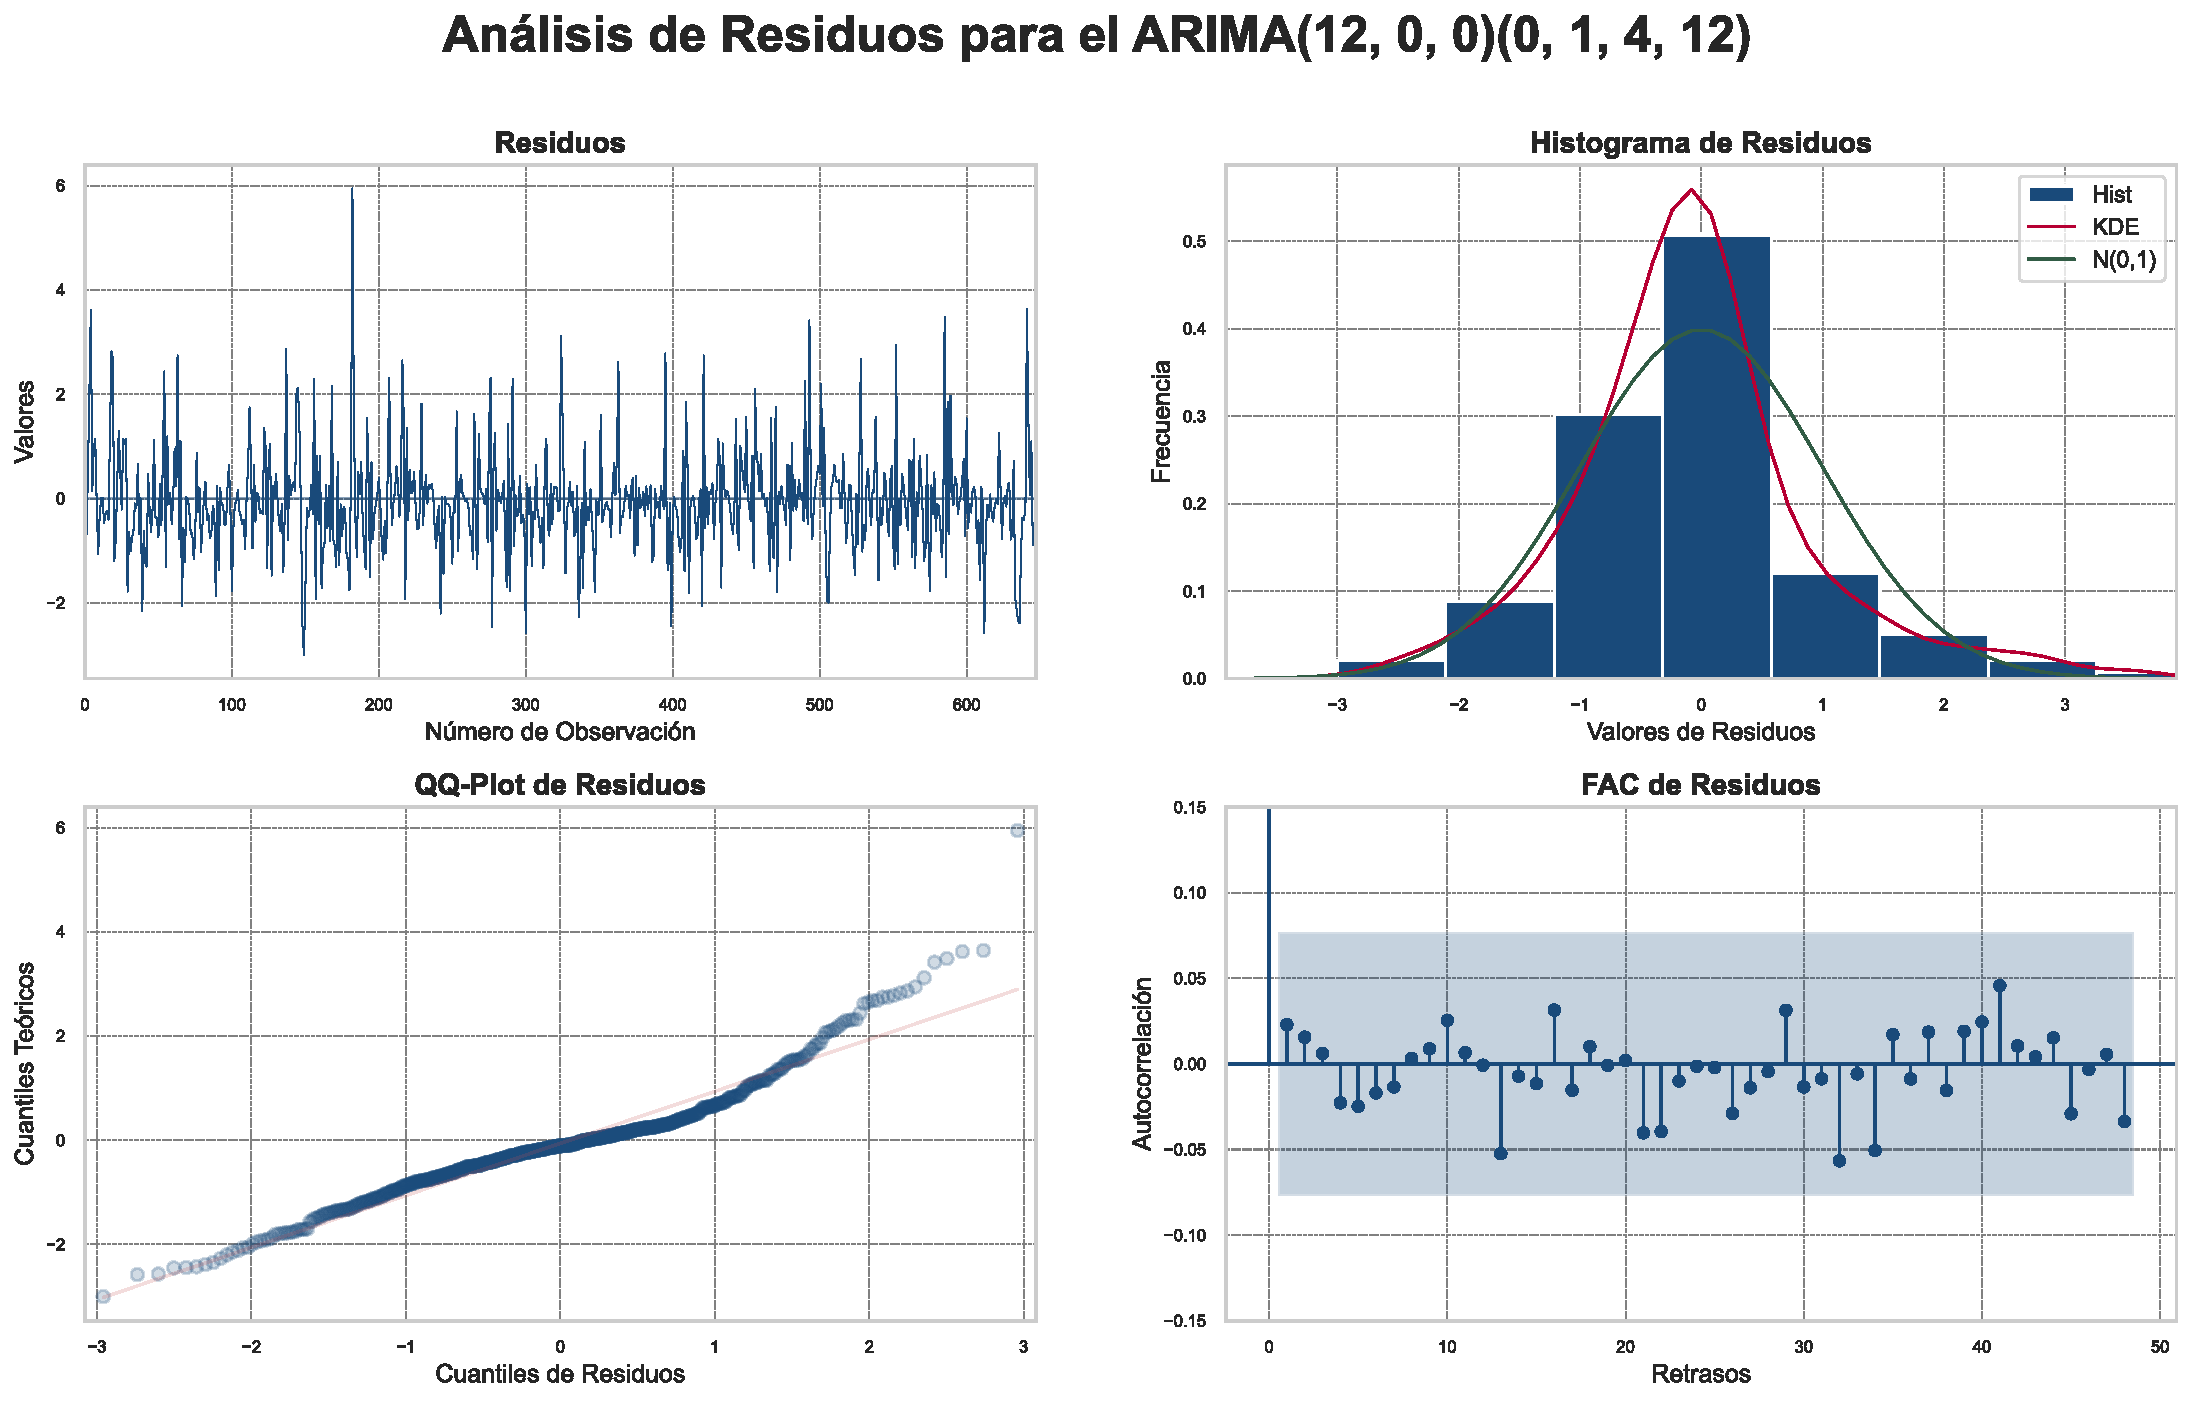
\includegraphics[width=0.8\textwidth]{imagenes/04-01-analisis-de-residuos-m1.pdf}
    \caption{\textit{Elaboración Propia}. FAC y FACP de la Primera Diferencia Estacional}
\end{figure}


\end{table}





\paragraph{Parsimonia}
El modelo no cumple con el principio de parsimonia, ya que cuenta con coeficientes que son altamente no significativos, como el $\phi_7$, con un p-valor de $0.923$, pero, aunque no pase el principio de parsimonia, dado que se intentó con otros 16 modelos de ordenes menores y ninguno cumplia la prueba de residuos independientes, se será flexible en cuanto a este principio.

\paragraph{Invertibilidad}  
El modelo es invertible, ya que las raíces del polinomio característico de la parte de media móvil (MA) tienen módulo mayor que uno, es decir, se encuentran fuera del círculo unitario en el plano complejo. A continuación se presentan los módulos de dichas raíces:

\[
\begin{array}{cccccc}
1.0931, & 1.0931, & 1.0653, & 1.0653, & 1.0010, & 1.0931, \\
1.0931, & 1.0653, & 1.0653, & 1.0653, & 1.0653, & 1.0010, \\
1.0010, & 1.0653, & 1.0653, & 1.0653, & 1.0653, & 1.0010, \\
1.0010, & 1.0931, & 1.0931, & 1.0653, & 1.0653, & 1.0653, \\
1.0653, & 1.0010, & 1.0010, & 1.0931, & 1.0931, & 1.0653, \\
1.0653, & 1.0653, & 1.0653, & 1.0010, & 1.0010, & 1.0931, \\
1.0931, & 1.0931, & 1.0931, & 1.0653, & 1.0653, & 1.0010, \\
1.0653, & 1.0653, & 1.0653, & 1.0653, & 1.0010, & 1.0010
\end{array}
\]

\paragraph{Estacionariedad}  
El modelo es estacionario, dado que las raíces del polinomio característico de la parte autorregresiva (AR) también tienen módulo mayor que uno, por lo tanto, también se encuentran fuera del círculo unitario. Los módulos correspondientes se muestran a continuación:

\[
\begin{array}{cccccc}
1.1158, & 1.0720, & 1.0720, & 1.0585, & 1.0585, & 1.0496, \\
1.0496, & 1.0654, & 1.0654, & 1.0680, & 1.0033, & 1.0033
\end{array}
\]



\paragraph{Residuos Independientes}
Las pruebas de residuos independientes fueron realizadas con Ljung-Box, los resultados se muestran en el Cuadro 2.

\begin{table}[ht]
\footnotesize
\centering
\begin{tabular}{ccc}
\hline
\textbf{} & \textbf{lb\_stat} & \textbf{lb\_pvalue} \\
\hline
16 & 8.652910 & NaN \\
17 & 8.961011 & 0.002758 \\
18 & 8.987107 & 0.011181 \\
19 & 8.989718 & 0.029428 \\
20 & 8.991484 & 0.061313 \\
21 & 9.423957 & 0.093303 \\
22 & 9.683789 & 0.138616 \\
23 & 9.688787 & 0.206906 \\
24 & 9.696828 & 0.286953 \\
25 & 9.696845 & 0.375580 \\
26 & 10.397531 & 0.406336 \\
27 & 11.023153 & 0.441326 \\
28 & 11.211664 & 0.510871 \\
29 & 11.644782 & 0.556964 \\
30 & 11.647451 & 0.634592 \\
31 & 11.649449 & 0.705346 \\
32 & 13.569215 & 0.630772 \\
33 & 13.606003 & 0.694769 \\
34 & 15.609204 & 0.619800 \\
35 & 15.631437 & 0.681709 \\
36 & 15.889978 & 0.723426 \\
\hline
\end{tabular}
\caption{\textit{Elaboración Propia}. Resultados de la prueba de Ljung-Box para los residuos}
\end{table}

El primer retraso tiene un  p-valor de 0.002758, debajo del umbral del 0.01, indicando evidencia estadísticamente significativa de autocorrelación no explicada por el modelo, sin embargo, es el único retraso menor a este umbral, a partir del retraso 4, el p-valor comienza a superar el 0.05 y sigue aumentando sucesivamente, lo que sugiere que no hay evidencia significativa de autocorrelación en esos retrasos. Aunque se espera que todos los residuos sean independientes, comparados con otros modelos, los p-valores obtenidos en este modelo son altos, por lo que se seguirá analizando.


\paragraph{Residuos con Media Cero}
Se realizó una prueba t para verificar si la media de los residuos es estadísticamente diferente de cero. El estadístico t obtenido fue $-1.6920$, con un p-valor de $0.0911$, y $659$ grados de libertad. Dado que el p-valor es mayor que el nivel de significancia, no se rechaza la hipótesis nula. Por lo tanto, se concluye que no hay evidencia suficiente para afirmar que la media de los residuos sea distinta de cero.

\paragraph{Residuos con Varianza Constante}
Se aplicó la prueba de Breusch-Pagan para evaluar si los residuos presentan varianza constante. El estadístico de la prueba fue $2.4640$ con un p-valor de $0.1165$. Dado que el p-valor es mayor que el nivel de significancia, no se rechaza la hipótesis nula de homoscedasticidad. Por lo tanto, se concluye que no hay evidencia suficiente para afirmar que los residuos presenten heterocedasticidad.

\paragraph{Residuos con Distribución Normal}
Se realizaron dos pruebas para evaluar si los residuos siguen una distribución normal:

\begin{itemize}
    \item Jarque-Bera: El estadístico fue $413.9383$ con un p-valor de $1.30 \times 10^{-90}$. Como el p-valor es mucho menor que $0.05$, se rechaza la hipótesis nula de normalidad según esta prueba.
    \item Lilliefors: El p-valor fue $0.0010$, por lo que también se rechaza la hipótesis nula de normalidad.
\end{itemize}

Dado que ambas pruebas rechazan la hipótesis nula, se concluye que los residuos no siguen una distribución normal. Sin embargo, se analiza la proporción de residuos que se encuentran dentro de ciertos múltiplos de la desviación estándar. Si los residuos fueran perfectamente normales, se esperaría aproximadamente un 68\% dentro de $\pm1\sigma$, un 95\% dentro de $\pm2\sigma$ y un 99.7\% dentro de $\pm3\sigma$. Los resultados observados son los siguientes:

\begin{itemize}
    \item 75.00\% de los residuos están dentro de $\pm1\sigma$ (esperado = 68\%),
    \item 93.79\% dentro de $\pm2\sigma$ (esperado = 95\%),
    \item 98.79\% dentro de $\pm3\sigma$ (esperado = 99.7\%).
\end{itemize}











\paragraph{Gráfico de los Residuos}
\begin{figure}[ht]
    \centering
    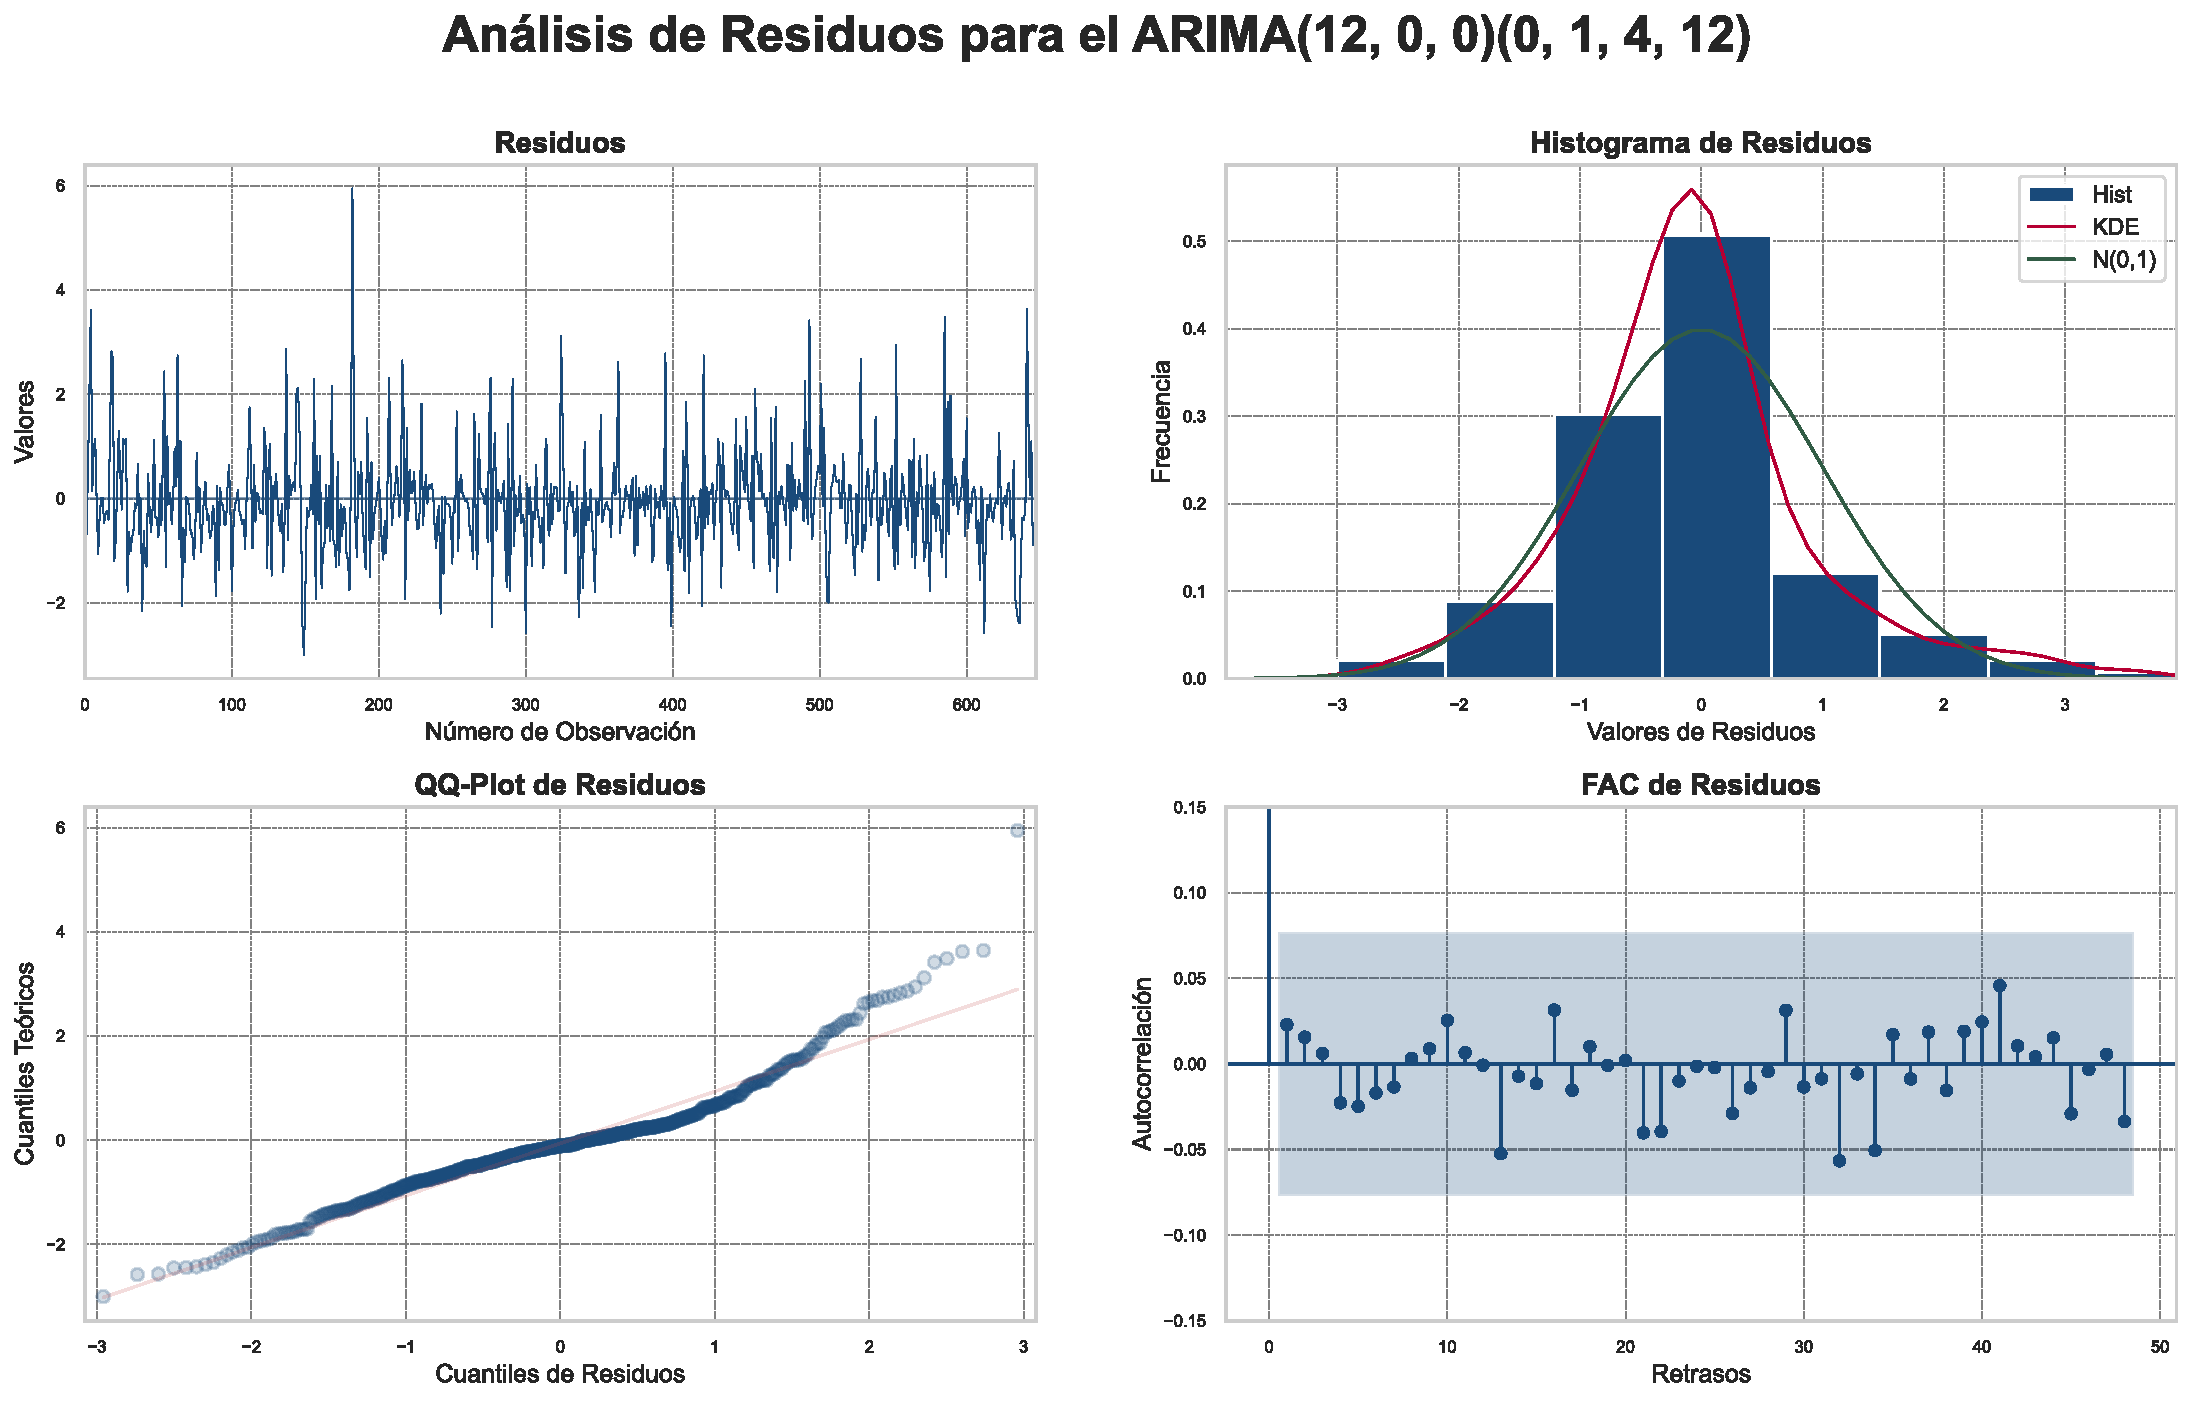
\includegraphics[width=0.8\textwidth]{imagenes/04-01-analisis-de-residuos-m1.pdf}
    \caption{\textit{Elaboración Propia}. Grafico de los Residuos del Primer Modelo}
\end{figure}

También se puede observar que los residuos tienen colas más pesadas que una distribución normal, lo bueno es claramente no hay correlación significativa entre ellos. 




\newpage


\subsubsection{Segundo Modelo para la Serie Sin Transformar}
Se propone el siguiente modelo encontrado con menor AIC.

\begin{table}[htbp]
\centering
\tiny
\caption{\textit{Elaboración Propia}. Segundo Modelo para la Serie Sin Transformar}
\begin{tabular}{llcl}
\toprule
Dep. Variable: & y & No. Observations: & 660 \\
Model: & SARIMAX(13, 0, 0)$\times$(0, 1, [1, 2, 3, 4], 12) & Log Likelihood & -665.685 \\
Date: & Sun, 27 Apr 2025 & AIC & 1367.369 \\
Time: & 04:49:22 & BIC & 1447.899 \\
Sample: & 0 & HQIC & 1398.609 \\
        & - 660 & & \\
Covariance Type: & opg & & \\
\bottomrule
\end{tabular}

\vspace{0.3cm}

\begin{tabular}{lrrrrrr}
\toprule
 & \textbf{coef} & \textbf{std err} & \textbf{z} & \textbf{P$>|z|$} & \textbf{[0.025} & \textbf{0.975]} \\
\midrule
ar.L1     & 0.1369 & 0.035 & 3.963  & 0.000 & 0.069 & 0.205 \\
ar.L2     & -0.0190 & 0.036 & -0.522 & 0.602 & -0.090 & 0.052 \\
ar.L3     & 0.0501 & 0.037 & 1.363  & 0.173 & -0.022 & 0.122 \\
ar.L4     & -0.0697 & 0.042 & -1.662 & 0.097 & -0.152 & 0.013 \\
ar.L5     & -0.1117 & 0.050 & -2.254 & 0.024 & -0.209 & -0.015 \\
ar.L6     & -0.1101 & 0.060 & -1.839 & 0.066 & -0.227 & 0.007 \\
ar.L7     & -0.0104 & 0.051 & -0.205 & 0.838 & -0.110 & 0.089 \\
ar.L8     & -0.0511 & 0.044 & -1.170 & 0.242 & -0.137 & 0.034 \\
ar.L9     & 0.0331 & 0.035 & 0.944  & 0.345 & -0.036 & 0.102 \\
ar.L10    & -0.0093 & 0.033 & -0.281 & 0.778 & -0.074 & 0.055 \\
ar.L11    & 0.1034 & 0.037 & 2.802  & 0.005 & 0.031 & 0.176 \\
ar.L12    & 0.5385 & 0.080 & 6.699  & 0.000 & 0.381 & 0.696 \\
ar.L13    & -0.0460 & 0.041 & -1.115 & 0.265 & -0.127 & 0.035 \\
ma.S.L12  & -1.3756 & 0.100 & -13.725 & 0.000 & -1.572 & -1.179 \\
ma.S.L24  & 0.3674 & 0.086 & 4.275  & 0.000 & 0.199 & 0.536 \\
ma.S.L36  & 0.0973 & 0.060 & 1.635  & 0.102 & -0.019 & 0.214 \\
ma.S.L48  & -0.0784 & 0.039 & -1.994 & 0.046 & -0.155 & -0.001 \\
sigma2    & 0.4340 & 0.030 & 14.503 & 0.000 & 0.375 & 0.493 \\
\bottomrule
\end{tabular}

\vspace{0.3cm}

\begin{tabular}{llcl}
\toprule
Ljung-Box (L1) (Q): & 0.04 & Jarque-Bera (JB): & 347.08 \\
Prob(Q): & 0.85 & Prob(JB): & 0.00 \\
Heteroskedasticity (H): & 0.83 & Skew: & 0.87 \\
Prob(H) (two-sided): & 0.17 & Kurtosis: & 6.14 \\
\bottomrule
\end{tabular}

\end{table}











\paragraph{Parsimonia}
Este modelo tampoco cumple el principio de parsimonia, ya que tiene coeficientes con un p-valor de 0.838 o 0.778, lo que sugiere que el coeficiente no es significativamente distinto de cero. Esto implica que la variable asociada no aporta evidencia suficiente de tener un efecto real en la variable dependiente, y su inclusión en el modelo podría considerarse innecesaria, ya que incrementa su complejidad sin una mejora proporcional en el ajuste o la capacidad predictiva.


\paragraph{Invertibilidad}
El modelo es invertible, ya que las raíces del polinomio característico de la parte de media móvil se encuentran fuera del círculo unitario. A continuación se presentan los módulos de dichas raíces:
\[
\begin{array}{cccccc}
1.0935, & 1.0935, & 1.0626, & 1.0626, & 1.0014, & 1.0935, \\
1.0935, & 1.0626, & 1.0626, & 1.0626, & 1.0626, & 1.0014, \\
1.0014, & 1.0626, & 1.0626, & 1.0626, & 1.0626, & 1.0014, \\
1.0014, & 1.0935, & 1.0935, & 1.0626, & 1.0626, & 1.0626, \\
1.0626, & 1.0014, & 1.0014, & 1.0935, & 1.0935, & 1.0626, \\
1.0626, & 1.0626, & 1.0626, & 1.0014, & 1.0014, & 1.0935, \\
1.0935, & 1.0935, & 1.0935, & 1.0626, & 1.0626, & 1.0014, \\
1.0626, & 1.0626, & 1.0626, & 1.0626, & 1.0014, & 1.0014
\end{array}
\]

\paragraph{Estacionariedad}
El modelo es estacionario, ya que las raíces del polinomio característico de la parte autorregresiva también se ubican fuera del círculo unitario. Los módulos correspondientes son los siguientes:

\[
\begin{array}{cccccc}
11.8885, & 1.0996, & 1.0624, & 1.0624, & 1.0510, & 1.0510, \\
1.0476, & 1.0476, & 1.0636, & 1.0636, & 1.0675, & 1.0030, \\
1.0030
\end{array}
\]

\paragraph{Residuos Independientes}
Se realizó la prueba de Ljung-Box para determinar si hay dependencia en los residuos, los resultados se muestran en el Cuadro 4.
\begin{table}[ht]
\footnotesize
\centering
\begin{tabular}{ccc}
\hline
\textbf{Index} & \textbf{lb\_stat} & \textbf{lb\_pvalue} \\
\hline
17 & 6.774386 & NaN \\
18 & 6.783618 & 0.009200 \\
19 & 6.786944 & 0.033592 \\
20 & 6.809256 & 0.078232 \\
21 & 7.196463 & 0.125863 \\
22 & 7.428032 & 0.190703 \\
23 & 7.441854 & 0.281909 \\
24 & 7.447962 & 0.383773 \\
25 & 7.506681 & 0.483077 \\
26 & 8.263074 & 0.507868 \\
27 & 8.898238 & 0.541788 \\
28 & 9.010612 & 0.620913 \\
29 & 9.533962 & 0.656772 \\
30 & 9.544856 & 0.730662 \\
31 & 9.545139 & 0.794626 \\
32 & 11.177851 & 0.739888 \\
33 & 11.194537 & 0.797321 \\
34 & 13.243411 & 0.719745 \\
35 & 13.251323 & 0.776431 \\
36 & 13.698894 & 0.800953 \\
37 & 13.804935 & 0.840247 \\
\hline
\end{tabular}
\caption{\textit{Elaboración Propia}. Resultados de la prueba de Ljung-Box para los residuos}
\end{table}


El primer retraso tiene un p-valor de 0.009200, que está por debajo del umbral de 0.01 por 0.001. Esto indica evidencia estadísticamente significativa de autocorrelación no explicada por el modelo. El siguiente retraso, presenta un p-valor de 0.033592, que es mayor al del caso pasado,y, a partir del retraso 3, los p-valores comienzan a superar el 0.05 y continúan aumentando sucesivamente. Estos p-valores son relativamente altos, incluso mas altos que el modelo anterior, lo que sugiere un ajuste aceptable del modelo a partir de ese punto.



\paragraph{Residuos con Media Cero}
Se realizó una prueba t para verificar si la media de los residuos es estadísticamente diferente de cero. El estadístico t obtenido fue $-1.6519$, con un p-valor de $0.0990$, y $659$ grados de libertad. Dado que el p-valor es mayor que el nivel de significancia, no se rechaza la hipótesis nula. Por lo tanto, se concluye que no hay evidencia suficiente para afirmar que la media de los residuos sea distinta de cero.

\paragraph{Residuos con Varianza Constante}
Se aplicó la prueba de Breusch-Pagan para evaluar si los residuos presentan varianza constante. El estadístico de la prueba fue $2.2724$ con un p-valor de $0.1317$. Dado que el p-valor es mayor que el nivel de significancia, no se rechaza la hipótesis nula de homoscedasticidad. Por lo tanto, se concluye que no hay evidencia suficiente para afirmar que los residuos presenten heterocedasticidad.

\paragraph{Residuos con Distribución Normal}
Se realizaron dos pruebas para evaluar si los residuos siguen una distribución normal:

\begin{itemize}
    \item Jarque-Bera: El estadístico fue $380.3671$ con un p-valor de $2.54 \times 10^{-83}$. Como el p-valor es mucho menor que $0.05$, se rechaza la hipótesis nula de normalidad según esta prueba.
    \item Lilliefors: El p-valor fue $0.0010$, por lo que también se rechaza la hipótesis nula de normalidad.
\end{itemize}

Dado que ambas pruebas rechazan la hipótesis nula, se concluye que los residuos no siguen una distribución normal. Sin embargo, se analiza la proporción de residuos que se encuentran dentro de ciertos múltiplos de la desviación estándar. Si los residuos fueran perfectamente normales, se esperaría aproximadamente un 68\% dentro de $\pm1\sigma$, un 95\% dentro de $\pm2\sigma$ y un 99.7\% dentro de $\pm3\sigma$. Los resultados observados son los siguientes:

\begin{itemize}
    \item 75.15\% de los residuos están dentro de $\pm1\sigma$ (esperado = 68\%),
    \item 93.79\% dentro de $\pm2\sigma$ (esperado = 95\%),
    \item 98.94\% dentro de $\pm3\sigma$ (esperado = 99.7\%).
\end{itemize}

Estos resultados sugieren que los residuos presentan un comportamiento aproximadamente normal.




\paragraph{Gráfico de los Residuos}
\begin{figure}[ht]
    \centering
    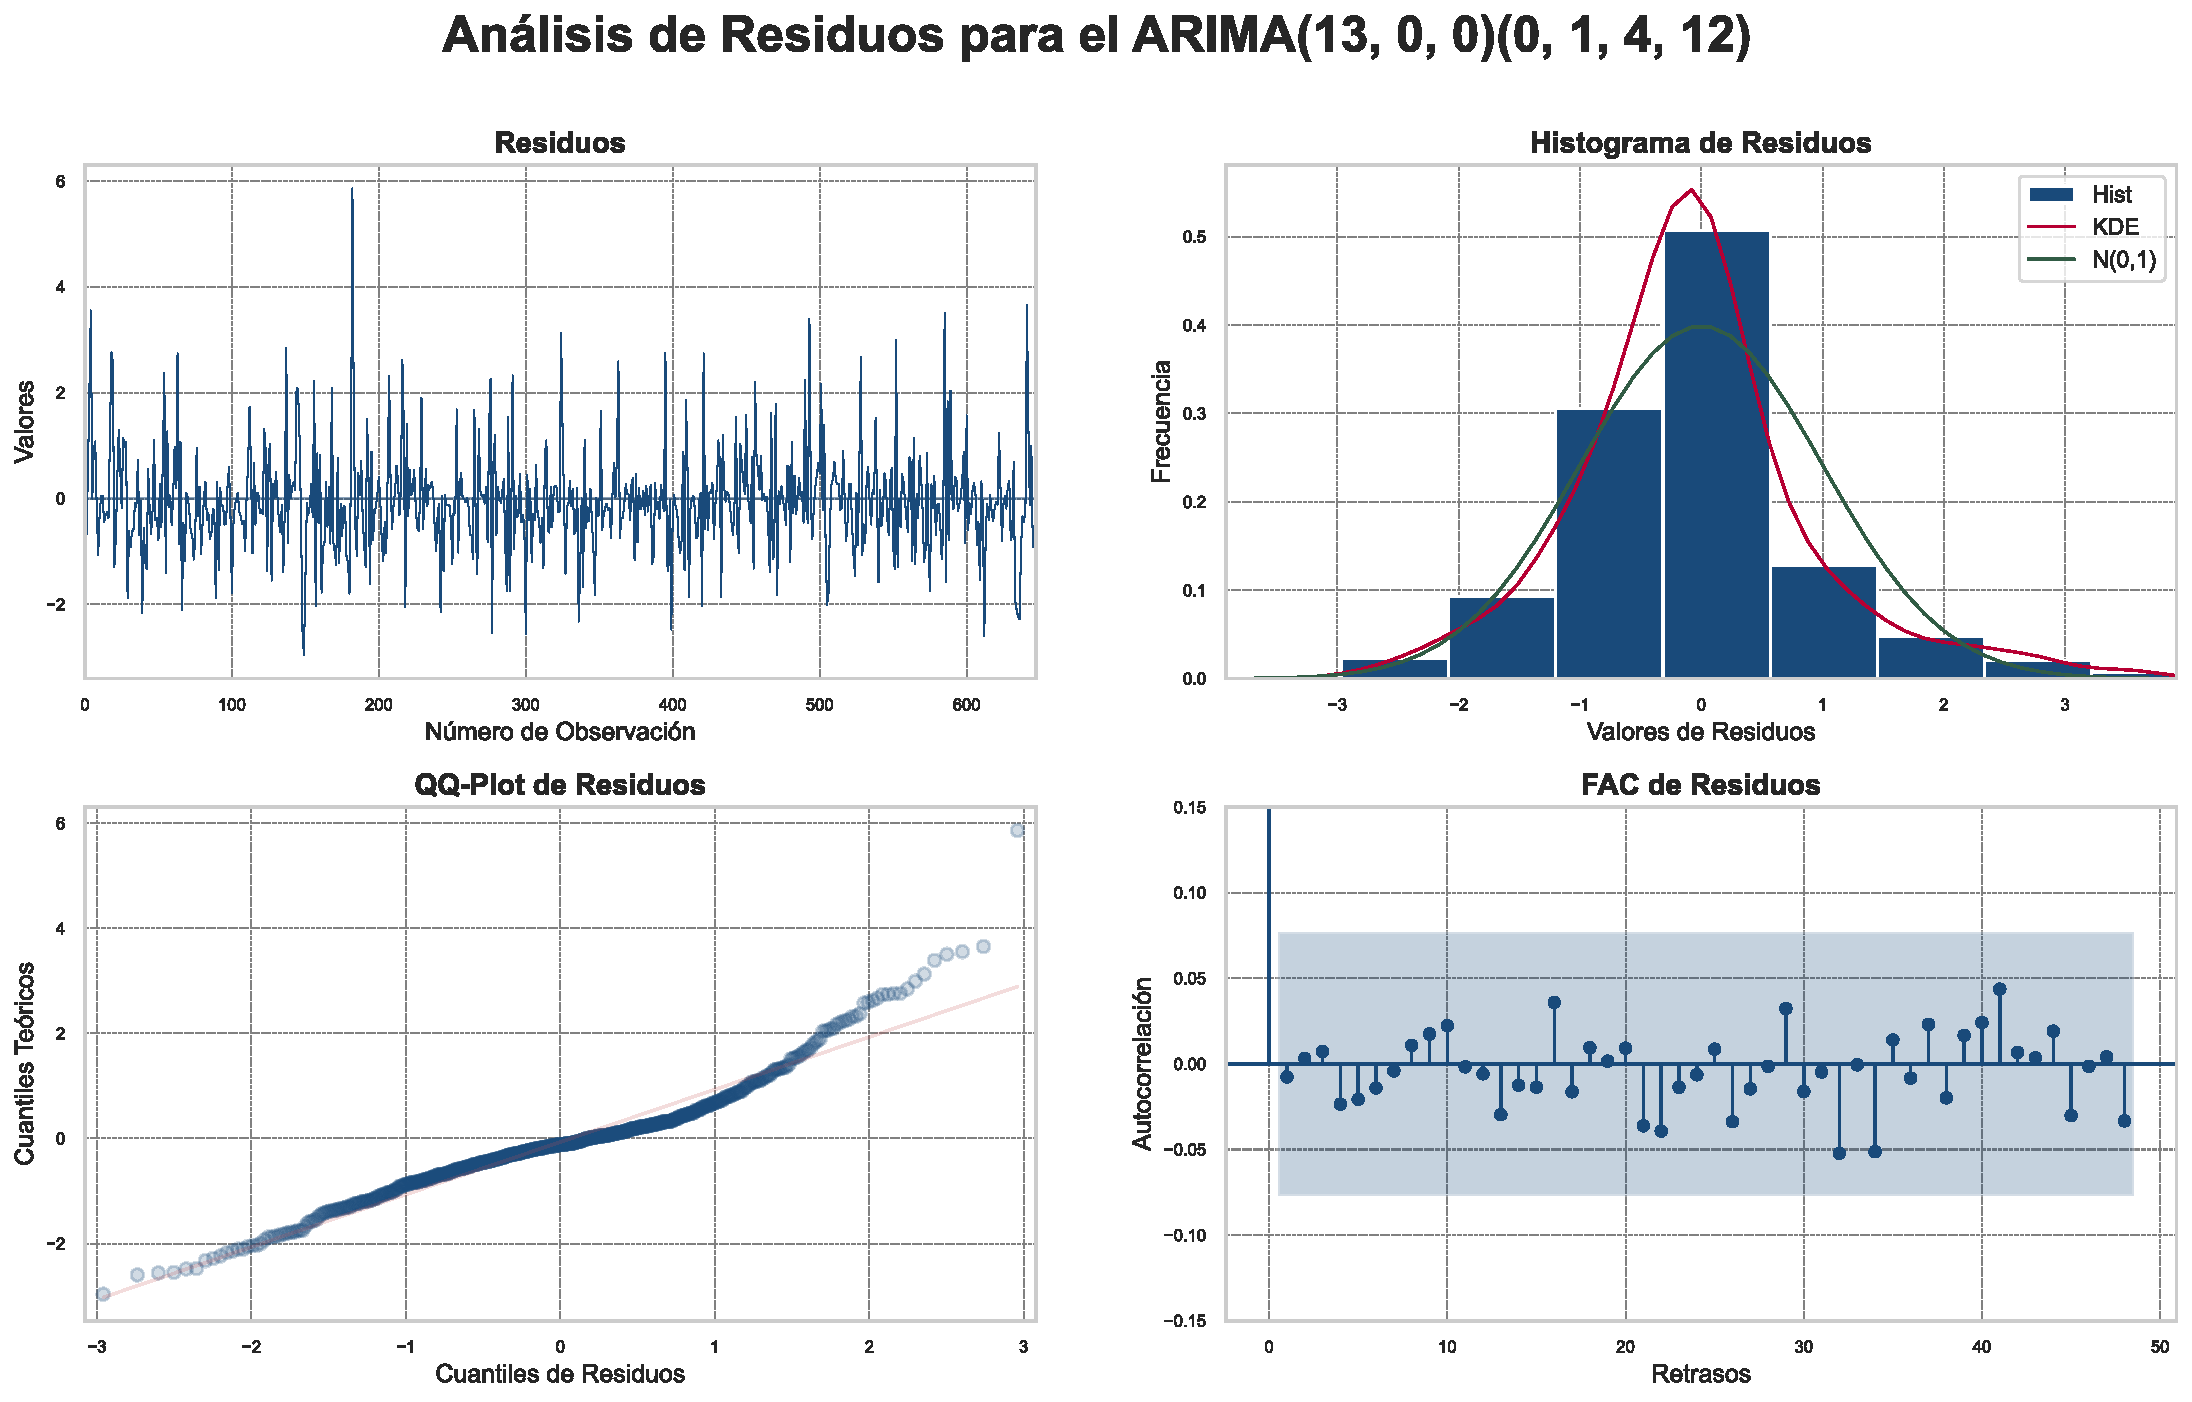
\includegraphics[width=0.8\textwidth]{imagenes/04-02-analisis-de-residuos-m2.pdf}
    \caption{\textit{Elaboración Propia}. Grafico de los Residuos del Primer Modelo}
\end{figure}

Ocurre lo mismo que en el caso pasado, los residuos tienen colas más pesadas.




















\newpage


\subsubsection{Tercer Modelo para la Serie Sin Transformar}

Tercer modelo encontrado con menor AIC.

\begin{table}[htbp]
\centering
\tiny
\caption{\textit{Elaboración Propia}. Tercer Modelo para la Serie Sin Transformar}
\begin{tabular}{llcl}
\toprule
Dep. Variable: & y & No. Observations: & 660 \\
Model: & SARIMAX(12, 0, 0)$\times$(0, 1, [1, 2], 12) & Log Likelihood & -668.499 \\
Date: & Sun, 27 Apr 2025 & AIC & 1366.998 \\
Time: & 04:49:32 & BIC & 1434.107 \\
Sample: & 0 & HQIC & 1393.032 \\
        & - 660 & & \\
Covariance Type: & opg & & \\
\bottomrule
\end{tabular}

\vspace{0.3cm}

\begin{tabular}{lrrrrrr}
\toprule
 & \textbf{coef} & \textbf{std err} & \textbf{z} & \textbf{P$>|z|$} & \textbf{[0.025} & \textbf{0.975]} \\
\midrule
ar.L1     & 0.1241 & 0.033 & 3.797  & 0.000 & 0.060 & 0.188 \\
ar.L2     & -0.0278 & 0.037 & -0.746 & 0.455 & -0.101 & 0.045 \\
ar.L3     & 0.0593 & 0.036 & 1.629  & 0.103 & -0.012 & 0.131 \\
ar.L4     & -0.0777 & 0.043 & -1.819 & 0.069 & -0.161 & 0.006 \\
ar.L5     & -0.1077 & 0.050 & -2.137 & 0.033 & -0.206 & -0.009 \\
ar.L6     & -0.1154 & 0.060 & -1.914 & 0.056 & -0.234 & 0.003 \\
ar.L7     & -0.0107 & 0.050 & -0.214 & 0.831 & -0.108 & 0.087 \\
ar.L8     & -0.0498 & 0.044 & -1.129 & 0.259 & -0.136 & 0.037 \\
ar.L9     & 0.0450 & 0.036 & 1.263  & 0.207 & -0.025 & 0.115 \\
ar.L10    & -0.0087 & 0.033 & -0.263 & 0.793 & -0.074 & 0.056 \\
ar.L11    & 0.1075 & 0.035 & 3.042  & 0.002 & 0.038 & 0.177 \\
ar.L12    & 0.5090 & 0.073 & 6.931  & 0.000 & 0.365 & 0.653 \\
ma.S.L12  & -1.3374 & 0.082 & -16.355 & 0.000 & -1.498 & -1.177 \\
ma.S.L24  & 0.3550 & 0.075 & 4.760  & 0.000 & 0.209 & 0.501 \\
sigma2    & 0.4394 & 0.022 & 20.157 & 0.000 & 0.397 & 0.482 \\
\bottomrule
\end{tabular}

\vspace{0.3cm}

\begin{tabular}{llcl}
\toprule
Ljung-Box (L1) (Q): & 0.11 & Jarque-Bera (JB): & 385.54 \\
Prob(Q): & 0.74 & Prob(JB): & 0.00 \\
Heteroskedasticity (H): & 0.82 & Skew: & 0.91 \\
Prob(H) (two-sided): & 0.15 & Kurtosis: & 6.31 \\
\bottomrule
\end{tabular}

\end{table}


\paragraph{Parsimonia}
Este modelo tampoco cumple el principio de parsimonia, ya que tiene coeficientes con un p-valor de 0.793. Cabe mencionar que se intentó eliminarlos, pero al hacerlo los modelos resultantes eran completamente diferentes.

\paragraph{Invertibilidad}
El modelo es invertible, ya que las raíces del polinomio característico de la parte de media móvil se encuentran fuera del círculo unitario. A continuación se presentan los módulos de dichas raíces:
\[
\begin{array}{cccccc}
1.0876, & 1.0023, & 1.0876, & 1.0876, & 1.0023, & 1.0023, \\
1.0876, & 1.0876, & 1.0023, & 1.0023, & 1.0876, & 1.0876, \\
1.0023, & 1.0023, & 1.0876, & 1.0876, & 1.0023, & 1.0023, \\
1.0876, & 1.0876, & 1.0876, & 1.0023, & 1.0023, & 1.0023
\end{array}
\]

\paragraph{Estacionariedad}
El modelo es estacionario, ya que las raíces del polinomio característico de la parte autorregresiva también se ubican fuera del círculo unitario. Los módulos correspondientes son los siguientes:

\[
\begin{array}{cccccc}
1.1241, & 1.0745, & 1.0745, & 1.0577, & 1.0577, & 1.0535, \\
1.0535, & 1.0679, & 1.0679, & 1.0635, & 1.0026, & 1.0026
\end{array}
\]


\paragraph{Residuos Independientes}
Se realizó la prueba de Ljung-Box para determinar si hay dependencia en los residuos, los resultados se muestran en el Cuadro 6.
\begin{table}[h!]
\footnotesize
\centering
\begin{tabular}{ccc}
\hline
\textbf{} & \textbf{lb\_stat} & \textbf{lb\_pvalue} \\
\hline
14 & 8.223545  & NaN \\
15 & 8.469831  & 0.003611 \\
16 & 8.751457  & 0.012579 \\
17 & 9.104454  & 0.027934 \\
18 & 9.135493  & 0.057801 \\
19 & 9.135514  & 0.103780 \\
20 & 9.139624  & 0.165877 \\
21 & 9.745116  & 0.203483 \\
22 & 10.168911 & 0.253370 \\
23 & 10.181542 & 0.335989 \\
24 & 10.580242 & 0.391141 \\
25 & 10.587480 & 0.478441 \\
26 & 11.470408 & 0.489092 \\
27 & 12.051651 & 0.523413 \\
28 & 12.201265 & 0.590143 \\
29 & 12.738996 & 0.622450 \\
30 & 12.744188 & 0.691362 \\
31 & 12.749628 & 0.752779 \\
32 & 14.953637 & 0.665148 \\
33 & 14.972683 & 0.724332 \\
34 & 17.346330 & 0.630384 \\
\hline
\end{tabular}
\caption{\textit{Elaboración Propia}. Resultados de la prueba de Ljung-Box para los residuos}
\end{table}

El primer retraso  muestra un p-valor de 0.003611, claramente por debajo del umbral de 0.01, lo que indica evidencia estadísticamente significativa de autocorrelación no explicada por el modelo. En los siguientes retrasos, los p-valores son parecidos a los otros dos modelos propuestos.



\paragraph{Residuos con Media Cero}
Se realizó una prueba t para verificar si la media de los residuos es estadísticamente diferente de cero. El estadístico t obtenido fue $-1.4907$, con un p-valor de $0.1365$, y $659$ grados de libertad. Dado que el p-valor es mayor que el nivel de significancia, no se rechaza la hipótesis nula. Por lo tanto, se concluye que no hay evidencia suficiente para afirmar que la media de los residuos sea distinta de cero.


\paragraph{Residuos con Varianza Constante}
Se aplicó la prueba de Breusch-Pagan para evaluar si los residuos presentan varianza constante. El estadístico de la prueba fue $2.3478$ con un p-valor de $0.1255$. Dado que el p-valor es mayor que el nivel de significancia, no se rechaza la hipótesis nula de homoscedasticidad. Por lo tanto, se concluye que no hay evidencia suficiente para afirmar que los residuos presenten heterocedasticidad.

\paragraph{Residuos con Distribución Normal}
Se realizaron dos pruebas para evaluar si los residuos siguen una distribución normal:

\begin{itemize}
    \item Jarque-Bera: El estadístico fue $421.1651$ con un p-valor de $3.51 \times 10^{-92}$. Como el p-valor es mucho menor que $0.05$, se rechaza la hipótesis nula de normalidad según esta prueba.
    \item Lilliefors: El p-valor fue $0.0010$, por lo que también se rechaza la hipótesis nula de normalidad.
\end{itemize}

Dado que ambas pruebas rechazan la hipótesis nula, se concluye que los residuos no siguen una distribución normal. Sin embargo, se analiza la proporción de residuos que se encuentran dentro de ciertos múltiplos de la desviación estándar. Si los residuos fueran perfectamente normales, se esperaría aproximadamente un 68\% dentro de $\pm1\sigma$, un 95\% dentro de $\pm2\sigma$ y un 99.7\% dentro de $\pm3\sigma$. Los resultados observados son los siguientes:

\begin{itemize}
    \item 75.15\% de los residuos están dentro de $\pm1\sigma$ (esperado = 68\%),
    \item 94.09\% dentro de $\pm2\sigma$ (esperado = 95\%),
    \item 98.79\% dentro de $\pm3\sigma$ (esperado = 99.7\%).
\end{itemize}





\paragraph{Gráfico de los Residuos}
\begin{figure}[ht]
    \centering
    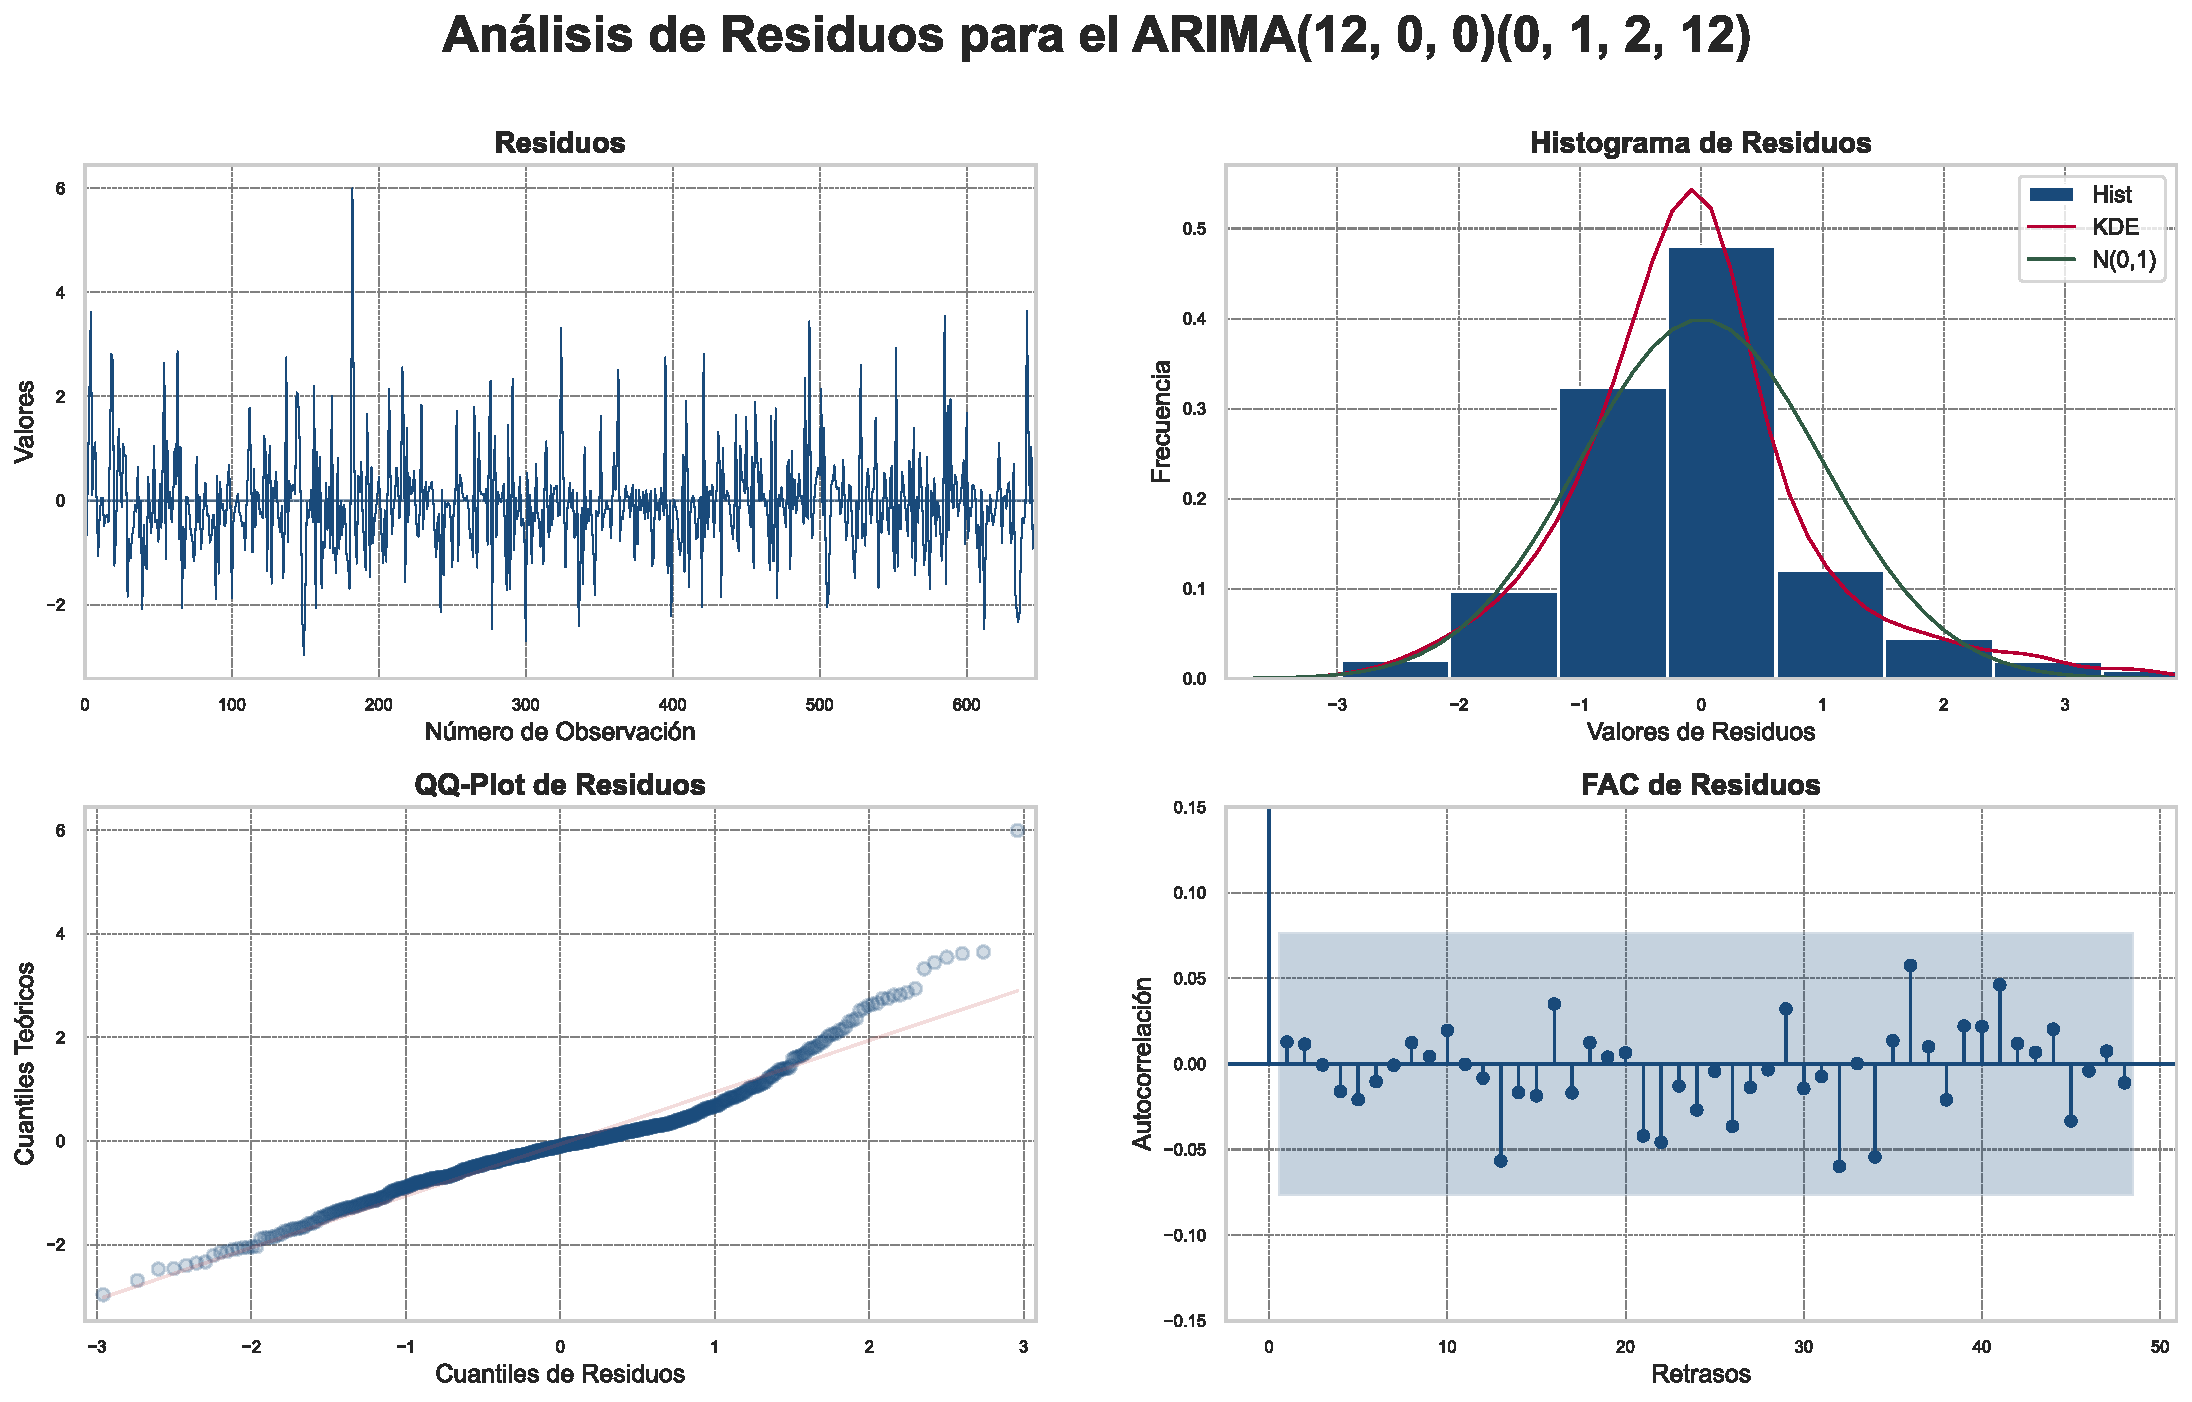
\includegraphics[width=0.8\textwidth]{imagenes/04-03-analisis-de-residuos-m3.pdf}
    \caption{\textit{Elaboración Propia}. Grafico de los Residuos del Tercer Modelo}
\end{figure}

Finalmente, se repite el mismo problema, colas pesadas en los residuos.




\newpage
$\quad$
\newpage
\subsubsection{Cuarto Modelo para la Serie Sin Transformar}

Dadas las funciones de autocorrelación simple y parcial, al intentar modelar, fue interesante encontrar este modelo:

\begin{table}[htbp]
\centering
\tiny
\caption{\textit{Elaboración Propia}. Cuarto Modelo para la Serie Sin Transformar}
\begin{tabular}{llcl}
\toprule
Dep. Variable: & y & No. Observations: & 660 \\
Model: & SARIMAX([1, 5], 0, [1, 5])$\times$(1, 1, 2, 12) & Log Likelihood & -5.099 \\
Date: & Sun, 27 Apr 2025 & AIC & 26.198 \\
Time: & 04:51:06 & BIC & 61.990 \\
Sample: & 0 & HQIC & 40.083 \\
        & - 660 & & \\
Covariance Type: & opg & & \\
\bottomrule
\end{tabular}

\vspace{0.3cm}

\begin{tabular}{lrrrrrr}
\toprule
 & \textbf{coef} & \textbf{std err} & \textbf{z} & \textbf{P$>|z|$} & \textbf{[0.025} & \textbf{0.975]} \\
\midrule
ar.L1     & 1.1476  & 32.468  & 0.035  & 0.972 & -62.489 & 64.784 \\
ar.L5     & -0.8775 & 38.486  & -0.023 & 0.982 & -76.308 & 74.553 \\
ma.L1     & -0.9317 & 23.880  & -0.039 & 0.969 & -47.736 & 45.872 \\
ma.L5     & 0.3314  & 36.742  & 0.009  & 0.993 & -71.681 & 72.344 \\
ar.S.L12  & -0.3697 & 133.649 & -0.003 & 0.998 & -262.317 & 261.577 \\
ma.S.L12  & -0.1630 & 41.007  & -0.004 & 0.997 & -80.536 & 80.210 \\
ma.S.L24  & -0.7558 & 42.337  & -0.018 & 0.986 & -83.735 & 82.223 \\
sigma2    & 0.4434  & 8.359   & 0.053  & 0.958 & -15.941 & 16.827 \\
\bottomrule
\end{tabular}


\vspace{0.3cm}

\begin{tabular}{llcl}
\toprule
Ljung-Box (L1) (Q): & 294.50 & Jarque-Bera (JB): & 2,134,861.83 \\
Prob(Q): & 0.00 & Prob(JB): & 0.00 \\
Heteroskedasticity (H): & 0.00 & Skew: & 15.72 \\
Prob(H) (two-sided): & 0.00 & Kurtosis: & 282.43 \\
\bottomrule
\end{tabular}
\end{table}

A pesar de que este modelo presenta el mejor valor de AIC entre todas las especificaciones consideradas, no cumple con ningún supuesto. Todos los parámetros estimados tienen p-valores superiores a 0.95, lo cual sugiere que no son significativamente distintos de cero. Además, los intervalos de confianza son demasiado amplios, lo cual indica una gran inestabilidad en las estimaciones. Esto podría deberse a una fuerte colinealidad entre regresores o a una sobreespecificación del modelo. La media de los residuos es de $-7.786026841214317\times10^{48}$, que puede deberse a inestabilidad numérica o un problema de precisión de punto flotante durante el proceso de optimización.

Una posible explicación para que este modelo tenga el menor AIC es que el criterio penaliza la complejidad, pero no exige validez . Esto demuestra la necesidad de no basarse únicamente en criterios de información, y de acompañar siempre la selección de modelos con un análisis de verificación de supuestos y estabilidad numérica.






















\newpage

\subsubsection{Primer Modelo Propuesto para la Serie Transformada}

Se intentó modelar con la FAC y la FACP, resultando el siguiente modelo:

\begin{table}[htbp]
\centering
\tiny
\caption{\textit{Elaboración Propia}. Primer Modelo Propuesto para la Serie Transformada}
\begin{tabular}{llcl}
\toprule
Dep. Variable: & y & No. Observations: & 660 \\
Model: & SARIMAX([1, 2, 6], 0, 1)$\times$(1, 1, [1, 2, 3, 4, 5, 6], 12) & Log Likelihood & -617.741 \\
Date: & Sun, 27 Apr 2025 & AIC & 1259.482 \\
Time: & 20:29:33 & BIC & 1313.169 \\
Sample: & 0 & HQIC & 1280.309 \\
        & - 660 & & \\
Covariance Type: & opg & & \\
\bottomrule
\end{tabular}

\vspace{0.3cm}

\begin{tabular}{lrrrrrr}
\toprule
 & \textbf{coef} & \textbf{std err} & \textbf{z} & \textbf{P$>|z|$} & \textbf{[0.025} & \textbf{0.975]} \\
\midrule
ar.L1     & 0.3566  & 0.144 & 2.482 & 0.013 & 0.075 & 0.638 \\
ar.L2     & 0.0211  & 0.062 & 0.342 & 0.732 & -0.100 & 0.142 \\
ar.L6     & -0.2754 & 0.036 & -7.653 & 0.000 & -0.346 & -0.205 \\
ma.L1     & -0.1092 & 0.149 & -0.731 & 0.465 & -0.402 & 0.184 \\
ar.S.L12  & -0.8536 & 0.246 & -3.468 & 0.001 & -1.336 & -0.371 \\
ma.S.L12  & 0.1009  & 0.245 & 0.412  & 0.680 & -0.379 & 0.581 \\
ma.S.L24  & -0.7034 & 0.191 & -3.691 & 0.000 & -1.077 & -0.330 \\
ma.S.L36  & 0.0214  & 0.049 & 0.435  & 0.664 & -0.075 & 0.118 \\
ma.S.L48  & 0.0154  & 0.054 & 0.286  & 0.775 & -0.090 & 0.121 \\
ma.S.L60  & 0.0169  & 0.053 & 0.319  & 0.750 & -0.087 & 0.121 \\
ma.S.L72  & 0.0063  & 0.055 & 0.114  & 0.909 & -0.101 & 0.114 \\
sigma2    & 0.3874  & 0.020 & 19.120 & 0.000 & 0.348  & 0.427 \\
\bottomrule
\end{tabular}

\vspace{0.3cm}

\begin{tabular}{llcl}
\toprule
Ljung-Box (L1) (Q): & 0.02 & Jarque-Bera (JB): & 10.86 \\
Prob(Q): & 0.88 & Prob(JB): & 0.00 \\
Heteroskedasticity (H): & 0.83 & Skew: & -0.20 \\
Prob(H) (two-sided): & 0.17 & Kurtosis: & 3.50 \\
\bottomrule
\end{tabular}

\end{table}


\paragraph{Residuos Independientes}
Se realizó la prueba de Ljung-Box para determinar si hay dependencia en los residuos, los resultados se muestran en el Cuadro 9.


\begin{table}[ht]
\footnotesize
\centering
\begin{tabular}{ccc}
\hline
\textbf{Index} & \textbf{lb\_stat} & \textbf{lb\_pvalue} \\
\hline
11 & 31.550176 & NaN \\
12 & 31.652621 & 1.843656e-08 \\
13 & 31.779184 & 1.256718e-07 \\
14 & 31.817201 & 5.718884e-07 \\
15 & 31.850384 & 2.052629e-06 \\
16 & 34.932704 & 1.551903e-06 \\
17 & 42.942269 & 1.197523e-07 \\
18 & 48.759895 & 2.528439e-08 \\
19 & 50.340543 & 3.514875e-08 \\
20 & 50.340543 & 9.294961e-08 \\
\hline
\end{tabular}
\caption{\textit{Elaboración Propia}. Resultados de la prueba de Ljung-Box para los residuos}
\end{table}


Los resultados presentados muestran una evidencia muy alta de autocorrelación en los residuos del modelo. Desde el retraso uno en adelante, todos los p-valores están muy por debajo del umbral (incluso 0.001). Estos valores indican que hay una fuerte dependencia temporal no capturada, y que los residuos no se comportan como ruido blanco. Por lo que no es necesario más análisis para este modelo, queda descartado.



\begin{figure}[ht]
    \centering
    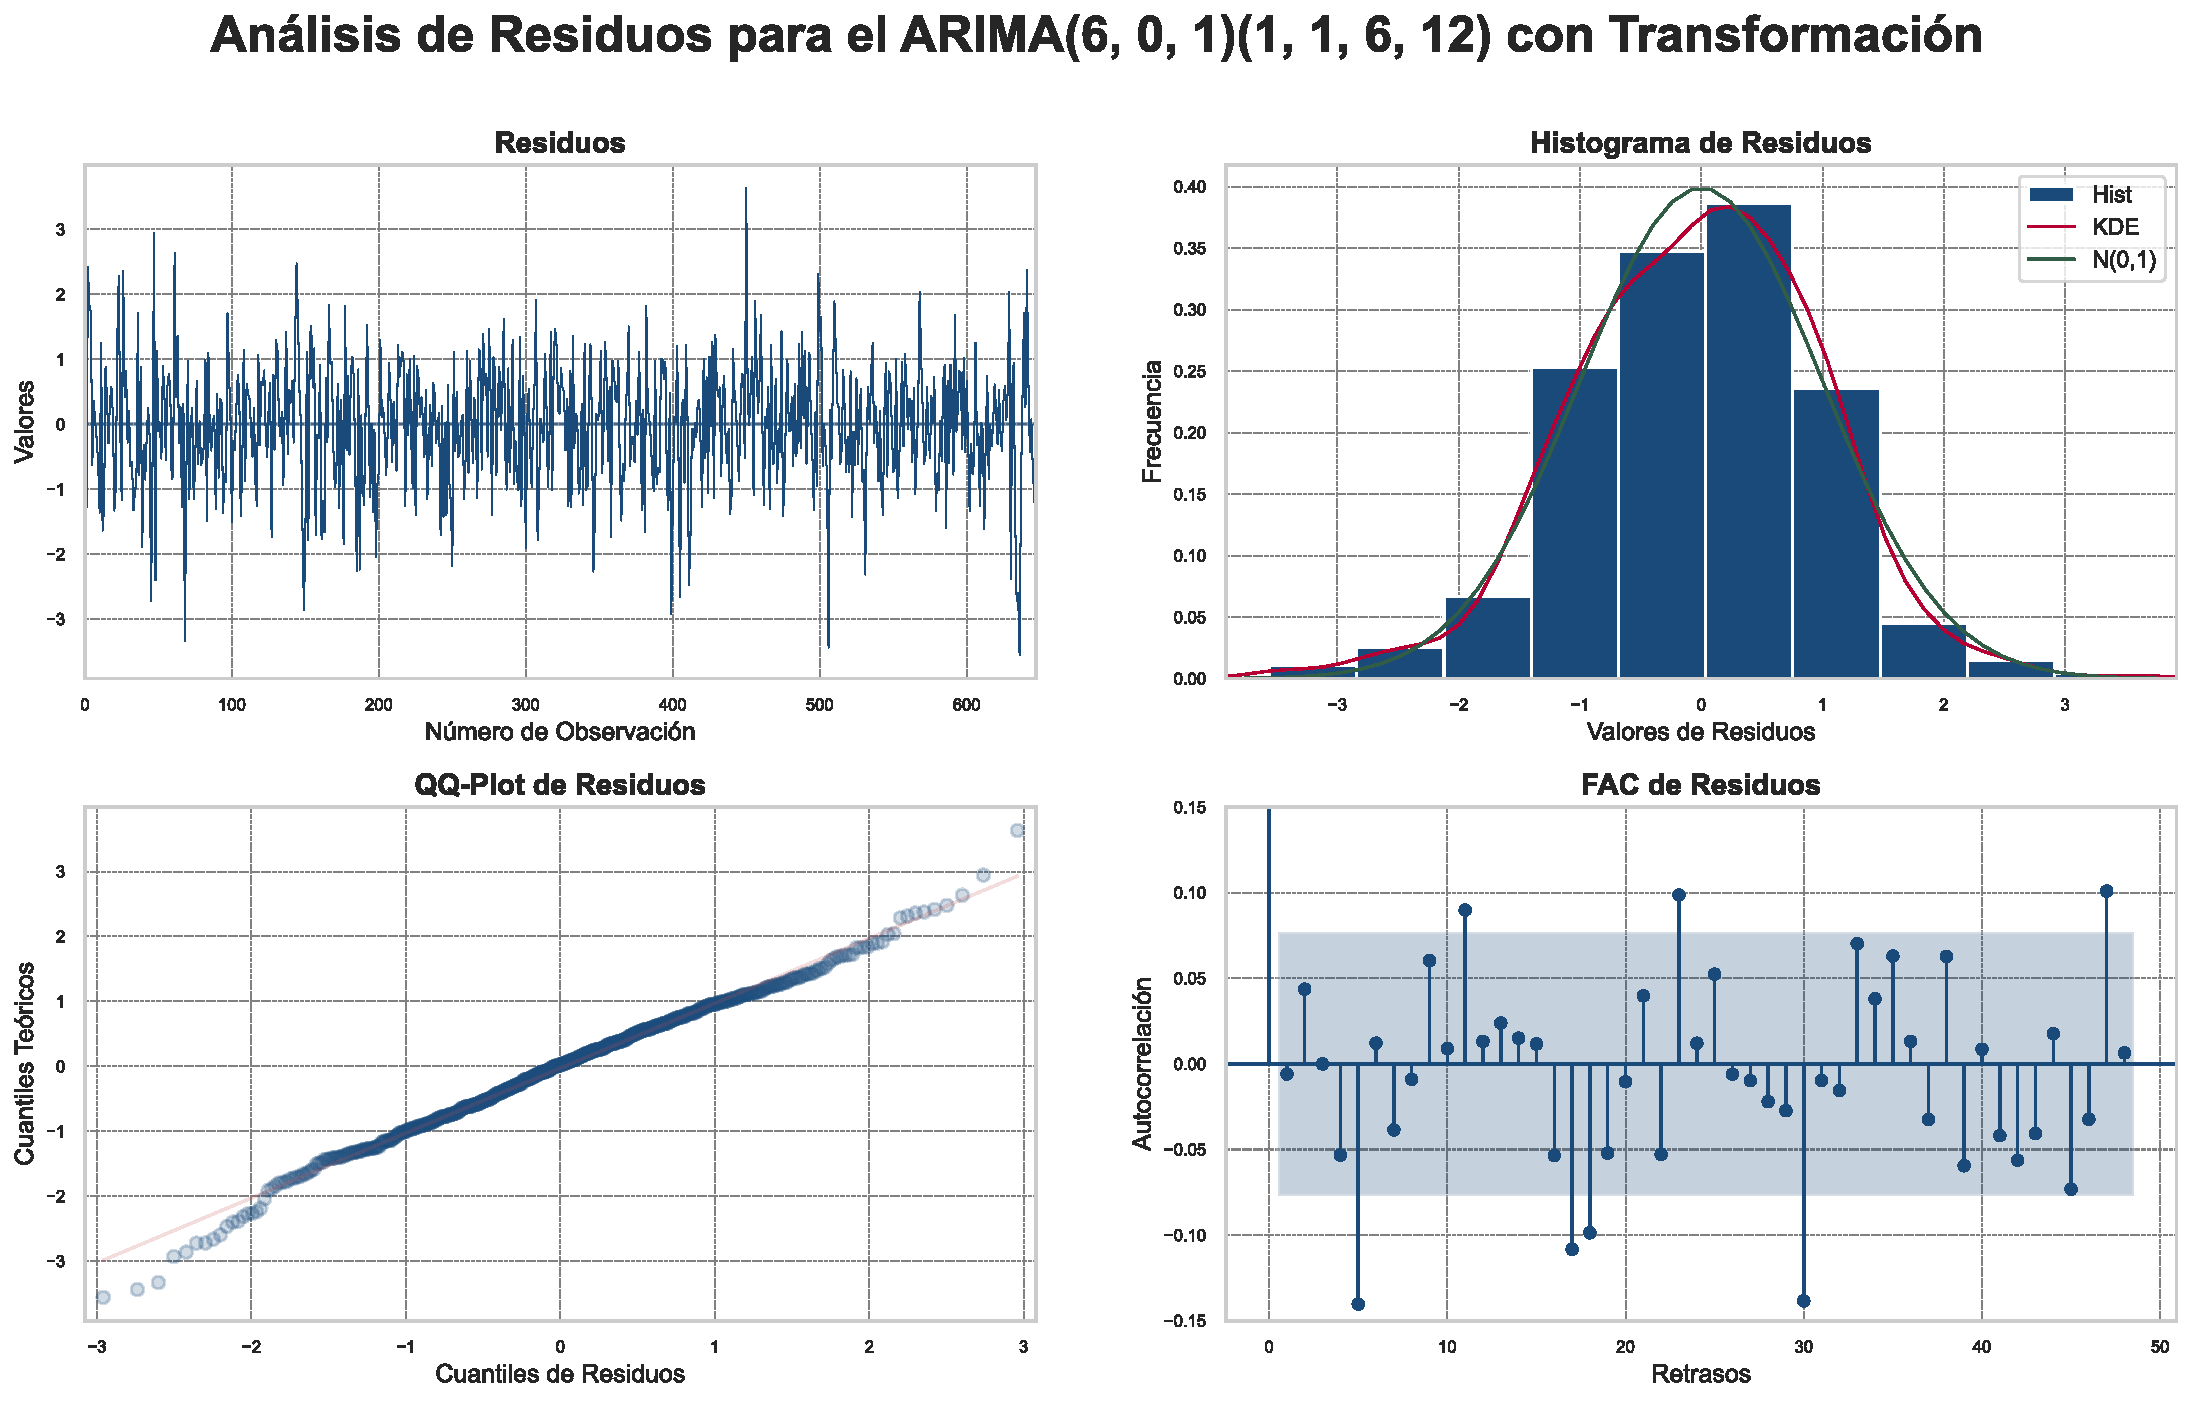
\includegraphics[width=0.8\textwidth]{imagenes/04-04-analisis-de-residuos-m1.pdf}
    \caption{\textit{Elaboración Propia}. Grafico de los Residuos para el Primer Modelo de la Serie Transformada}
\end{figure}

Por la dependencia en los residuos, cree que faltan parámetros para capturar de una forma más precisa la dependencia temporal de la serie.


\newpage
\subsubsection{Segundo Modelo Propuesto para la Serie Transformada}

A este modelo se llegó ajustando el modelo anterior, logrando el AIC menor entre todos los modelos.

\begin{table}[htbp]
\centering
\tiny
\caption{\textit{Elaboración Propia}. Segundo Modelo Propuesto para la Serie Transformada}
\begin{tabular}{llcl}
\toprule
Dep. Variable: & y & No. Observations: & 660 \\
Model: & SARIMAX(6, 0, 0)$\times$(1, 1, [1], 12) & Log Likelihood & -603.289 \\
Date: & Sun, 27 Apr 2025 & AIC & 1224.578 \\
Time: & 20:29:39 & BIC & 1264.843 \\
Sample: & 0 & HQIC & 1240.198 \\
        & - 660 & & \\
Covariance Type: & opg & & \\
\bottomrule
\end{tabular}

\vspace{0.3cm}

\begin{tabular}{lrrrrrr}
\toprule
 & \textbf{coef} & \textbf{std err} & \textbf{z} & \textbf{P$>|z|$} & \textbf{[0.025} & \textbf{0.975]} \\
\midrule
ar.L1     & 0.2721 & 0.034 & 7.929 & 0.000 & 0.205 & 0.339 \\
ar.L2     & 0.1022 & 0.041 & 2.473 & 0.013 & 0.021 & 0.183 \\
ar.L3     & -0.0255 & 0.040 & -0.644 & 0.520 & -0.103 & 0.052 \\
ar.L4     & -0.0900 & 0.041 & -2.215 & 0.027 & -0.170 & -0.010 \\
ar.L5     & -0.1974 & 0.039 & -5.011 & 0.000 & -0.275 & -0.120 \\
ar.L6     & -0.2604 & 0.038 & -6.796 & 0.000 & -0.336 & -0.185 \\
ar.S.L12  & 0.0196 & 0.046 & 0.426  & 0.670 & -0.071 & 0.110 \\
ma.S.L12  & -0.8851 & 0.029 & -30.327 & 0.000 & -0.942 & -0.828 \\
sigma2    & 0.3670 & 0.019 & 19.130 & 0.000 & 0.329 & 0.405 \\
\bottomrule
\end{tabular}

\vspace{0.3cm}

\begin{tabular}{llcl}
\toprule
Ljung-Box (L1) (Q): & 0.22 & Jarque-Bera (JB): & 6.43 \\
Prob(Q): & 0.64 & Prob(JB): & 0.04 \\
Heteroskedasticity (H): & 0.80 & Skew: & -0.19 \\
Prob(H) (two-sided): & 0.10 & Kurtosis: & 3.30 \\
\bottomrule
\end{tabular}

\end{table}


\paragraph{Parsimonia}
Aunque este modelo es el que tiene menos coeficientes en comparación a todos los demás, tampoco cumple el principio de parsimonia, teniendo coeficientes con un p-valor de 0.67. 


\paragraph{Invertibilidad}
El modelo es invertible, ya que las raíces del polinomio característico de la parte de media móvil se encuentran fuera del círculo unitario. A continuación se presentan los módulos de dichas raíces:
\[
\begin{array}{cccccc}
1.0102, & 1.0102, & 1.0102, & 1.0102, & 1.0102, & 1.0102, \\
1.0102, & 1.0102, & 1.0102, & 1.0102, & 1.0102, & 1.0102
\end{array}
\]

\paragraph{Estacionariedad}
El modelo es estacionario, ya que las raíces del polinomio característico de la parte autorregresiva también se ubican fuera del círculo unitario. Los módulos correspondientes son los siguientes:

\[
\begin{array}{cccccc}
1.5325, & 1.5648, & 1.5648, & 1.3008, & 1.3008, & 1.6452, \\
1.6452, & 1.2588, & 1.2588, & 1.6720, & 1.0589, & 1.0589
\end{array}
\]

\paragraph{Residuos Independientes}
Se realizó la prueba de Ljung-Box para determinar si hay dependencia en los residuos, los resultados se muestran en el Cuadro 11.
\begin{table}[ht]
\footnotesize
\centering
\begin{tabular}{ccc}
\hline
\textbf{Index} & \textbf{lb\_stat} & \textbf{lb\_pvalue} \\
\hline
9 & 6.473299 & NaN \\
10 & 7.880155 & 0.004998 \\
11 & 9.034590 & 0.010919 \\
12 & 9.198592 & 0.026764 \\
13 & 9.646686 & 0.046819 \\
14 & 9.995740 & 0.075356 \\
15 & 10.036647 & 0.123117 \\
16 & 10.813321 & 0.146972 \\
17 & 20.147979 & 0.009790 \\
18 & 24.051508 & 0.004221 \\
19 & 24.928482 & 0.005483 \\
20 & 25.176289 & 0.008590 \\
21 & 25.707594 & 0.011804 \\
22 & 30.300176 & 0.004262 \\
23 & 32.585774 & 0.003304 \\
24 & 32.718036 & 0.005134 \\
25 & 33.218651 & 0.006912 \\
26 & 33.280245 & 0.010384 \\
27 & 33.486398 & 0.014565 \\
28 & 33.781554 & 0.019498 \\
29 & 33.785406 & 0.027614 \\
\hline
\end{tabular}
\caption{\textit{Elaboración Propia}. Resultados de la prueba de Ljung-Box para los residuos}
\end{table}

Es interesante notar que el primer retraso tiene un p-valor de 0.004998 y se incrementa hasta el retraso 7, el p-valor sube a 0.14 y luego de este punto, los p-valores vuelven a caer, en el retraso 12, se muestran retrasos por debajo de 0.01, por ejemplo, 0.009790, lo que indica que la autocorrelación persiste de forma significativa en los retrasos más altos. 

\paragraph{Residuos con Media Cero}
Se realizó una prueba t para verificar si la media de los residuos es estadísticamente diferente de cero. El estadístico t obtenido fue $-1.3521$, con un p-valor de $0.1768$, y $659$ grados de libertad. Dado que el p-valor es mayor que el umbral, no se rechaza la hipótesis nula. Por lo tanto, se concluye que no hay evidencia suficiente para afirmar que la media de los residuos sea distinta de cero.

\paragraph{Residuos con Varianza Constante}
Se aplicó la prueba de Breusch-Pagan para evaluar si los residuos presentan varianza constante. El estadístico de la prueba fue $8.5927$ con un p-valor de $0.0034$. Dado que el p-valor es menor que el umbral, se rechaza la hipótesis nula de homoscedasticidad. Por lo tanto, se concluye que los residuos no presentan varianza constante, es decir, hay evidencia de heterocedasticidad.

\paragraph{Residuos con Distribución Normal}
Se realizaron dos pruebas para evaluar si los residuos siguen una distribución normal:

\begin{itemize}
    \item Jarque-Bera: El estadístico fue $6.6930$ con un p-valor de $0.0352$. Siendo muy estríctos, como se fijó un nivel de significancia antes de realizar las pruebas, y el p-valor es menor que $0.05$, se rechaza la hipótesis nula de normalidad según esta prueba.
    \item Lilliefors: El p-valor fue $0.3748$, por lo que no se rechaza la hipótesis nula de normalidad.
\end{itemize}

Dado que las pruebas ofrecen resultados contradictorios, no se puede concluir con certeza que los residuos sigan o no una distribución normal. Sin embargo, la evidencia a favor de la no normalidad no es concluyente. Por lo que se analiza la proporción de residuos que se encuentran dentro de ciertos múltiplos de la desviación estándar. Si los residuos fueran perfectamente normales, se esperaría aproximadamente un 68\% dentro de $\pm1\sigma$, un 95\% dentro de $\pm2\sigma$ y un 99.7\% dentro de $\pm3\sigma$. Los resultados observados son los siguientes:

\begin{itemize}
    \item 70.00\% de los residuos están dentro de $\pm1\sigma$ (esperado = 68\%),
    \item 95.30\% dentro de $\pm2\sigma$ (esperado = 95\%),
    \item 99.55\% dentro de $\pm3\sigma$ (esperado = 99.7\%).
\end{itemize}

Estos resultados sugieren que los residuos se comportan de manera aproximadamente normal, más que en los otros modelos.

\begin{figure}[ht]
    \centering
    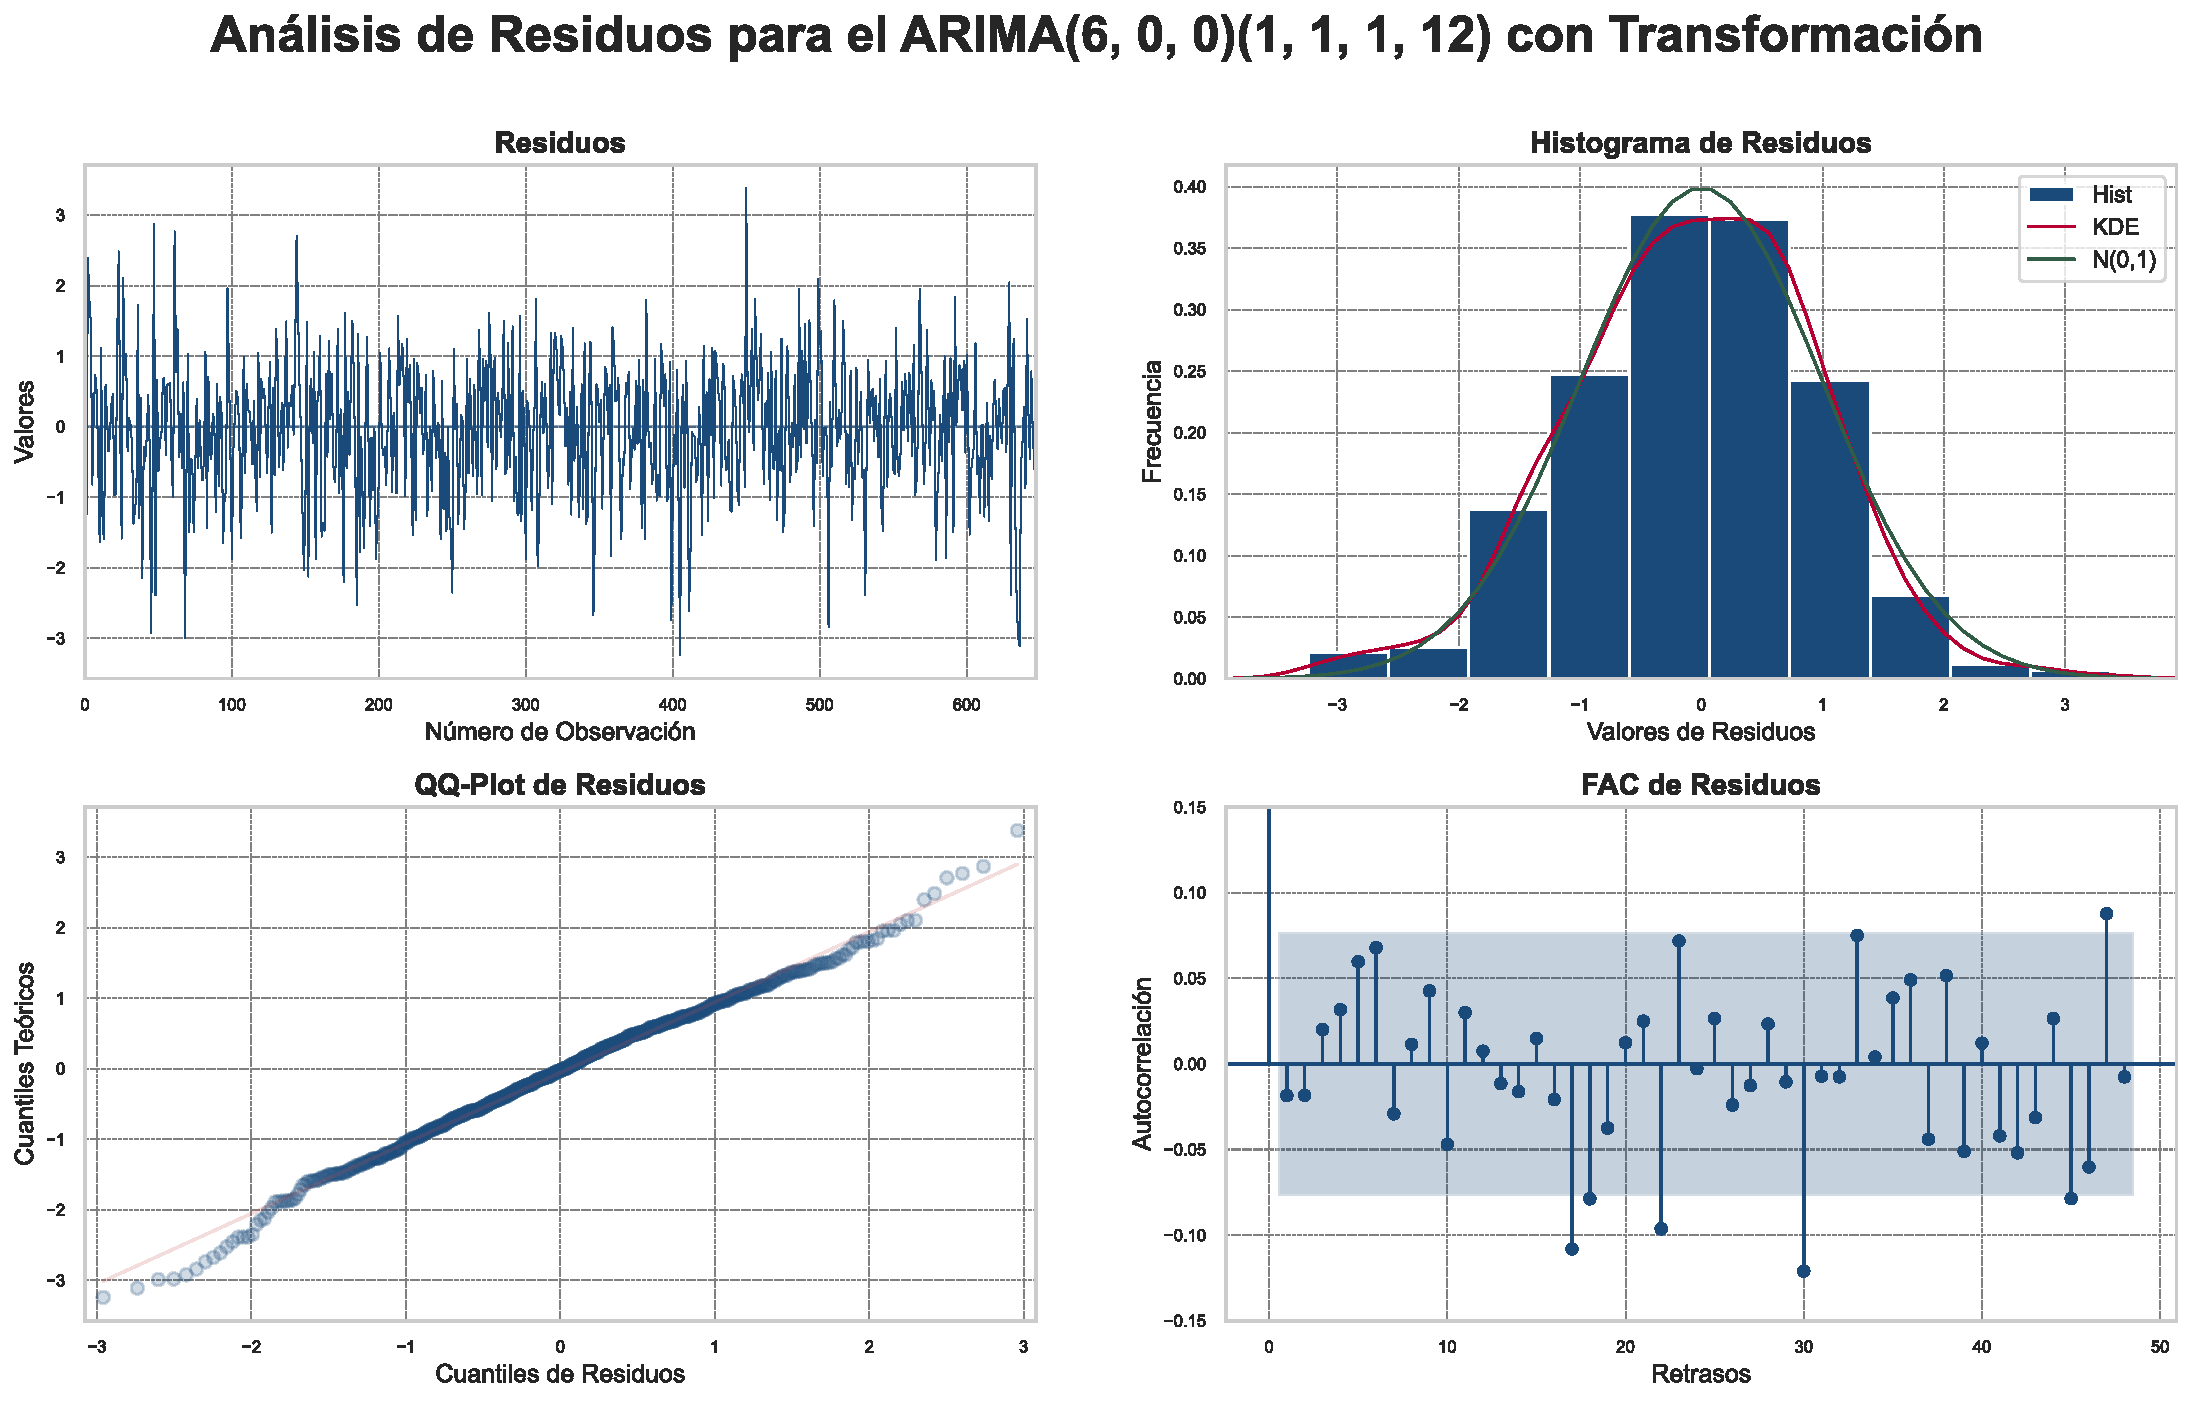
\includegraphics[width=0.8\textwidth]{imagenes/04-05-analisis-de-residuos-m3.pdf}
    \caption{\textit{Elaboración Propia}. Grafico de los Residuos para el Segundo Modelo de la Serie Transformada}
\end{figure}

Se puede ver en la figuro 25 que, efectivamente, los residuos están altamente correlacionados a partir del retraso 17, pero su distribución de residuos sí podría ser una normal.

































\newpage
$\quad$
\newpage
\subsection{Modelo Seleccionado}
Entre los modelos que fueron tratados en la sección anterior, se seleccionó el que se cree tiene la capacidad para modelar mejor la serie de tiempo de la precipitación, que, aunque no cumple el principio de parsimonia, ni pasa el test de normalidad de Jarque Bera ni el de Lilliefors, pero es el que tiene los p-valores del test de Ljung-Box más altos, indicando que es el más capaz de contener la información temporal sobre la serie.
\begin{table}[htbp]
\centering
\tiny
\caption{\textit{Elaboración Propia}. Modelo Seleccionado para la Serie Sin Transformar}
\begin{tabular}{llcl}
\toprule
Dep. Variable: & y & No. Observations: & 660 \\
Model: & SARIMAX(13, 0, 0)$\times$(0, 1, [1, 2, 3, 4], 12) & Log Likelihood & -665.685 \\
Date: & Sun, 27 Apr 2025 & AIC & 1367.369 \\
Time: & 04:49:22 & BIC & 1447.899 \\
Sample: & 0 & HQIC & 1398.609 \\
        & - 660 & & \\
Covariance Type: & opg & & \\
\bottomrule
\end{tabular}

\vspace{0.3cm}


\begin{tabular}{lrrrrrr}
\toprule
 & \textbf{coef} & \textbf{std err} & \textbf{z} & \textbf{P$>|z|$} & \textbf{[0.025} & \textbf{0.975]} \\
\midrule
ar.L1     & 0.1369 & 0.035 & 3.963  & 0.000 & 0.069 & 0.205 \\
ar.L2     & -0.0190 & 0.036 & -0.522 & 0.602 & -0.090 & 0.052 \\
ar.L3     & 0.0501 & 0.037 & 1.363  & 0.173 & -0.022 & 0.122 \\
ar.L4     & -0.0697 & 0.042 & -1.662 & 0.097 & -0.152 & 0.013 \\
ar.L5     & -0.1117 & 0.050 & -2.254 & 0.024 & -0.209 & -0.015 \\
ar.L6     & -0.1101 & 0.060 & -1.839 & 0.066 & -0.227 & 0.007 \\
ar.L7     & -0.0104 & 0.051 & -0.205 & 0.838 & -0.110 & 0.089 \\
ar.L8     & -0.0511 & 0.044 & -1.170 & 0.242 & -0.137 & 0.034 \\
ar.L9     & 0.0331 & 0.035 & 0.944  & 0.345 & -0.036 & 0.102 \\
ar.L10    & -0.0093 & 0.033 & -0.281 & 0.778 & -0.074 & 0.055 \\
ar.L11    & 0.1034 & 0.037 & 2.802  & 0.005 & 0.031 & 0.176 \\
ar.L12    & 0.5385 & 0.080 & 6.699  & 0.000 & 0.381 & 0.696 \\
ar.L13    & -0.0460 & 0.041 & -1.115 & 0.265 & -0.127 & 0.035 \\
ma.S.L12  & -1.3756 & 0.100 & -13.725 & 0.000 & -1.572 & -1.179 \\
ma.S.L24  & 0.3674 & 0.086 & 4.275  & 0.000 & 0.199 & 0.536 \\
ma.S.L36  & 0.0973 & 0.060 & 1.635  & 0.102 & -0.019 & 0.214 \\
ma.S.L48  & -0.0784 & 0.039 & -1.994 & 0.046 & -0.155 & -0.001 \\
sigma2    & 0.4340 & 0.030 & 14.503 & 0.000 & 0.375 & 0.493 \\
\bottomrule
\end{tabular}
\end{table}






Se comparará con el segundo modelo que fue entrenado con la transformación, dado que sí cumple con el test de Lilliefors y en Jarque Bera tiene un p-valor de 0.03, tiene un menor AIC, pero el único supuesto de los residuos que cumple es normalidad (además del de media cero). Se creé que los intervalos de confianza podrían ser la mayor diferencia entre los modelos (por la normalidad).





\begin{table}[htbp]
\centering
\tiny
\caption{\textit{Elaboración Propia}. Modelo Seleccionado para la Serie Con Transformaciones}
\begin{tabular}{llcl}
\toprule
Dep. Variable: & y & No. Observations: & 660 \\
Model: & SARIMAX(6, 0, 0)$\times$(1, 1, [1], 12) & Log Likelihood & -603.289 \\
Date: & Sun, 27 Apr 2025 & AIC & 1224.578 \\
Time: & 20:29:39 & BIC & 1264.843 \\
Sample: & 0 & HQIC & 1240.198 \\
        & - 660 & & \\
Covariance Type: & opg & & \\
\bottomrule
\end{tabular}

\vspace{0.3cm}

\begin{tabular}{lrrrrrr}
\toprule
 & \textbf{coef} & \textbf{std err} & \textbf{z} & \textbf{P$>|z|$} & \textbf{[0.025} & \textbf{0.975]} \\
\midrule
ar.L1     & 0.2721 & 0.034 & 7.929 & 0.000 & 0.205 & 0.339 \\
ar.L2     & 0.1022 & 0.041 & 2.473 & 0.013 & 0.021 & 0.183 \\
ar.L3     & -0.0255 & 0.040 & -0.644 & 0.520 & -0.103 & 0.052 \\
ar.L4     & -0.0900 & 0.041 & -2.215 & 0.027 & -0.170 & -0.010 \\
ar.L5     & -0.1974 & 0.039 & -5.011 & 0.000 & -0.275 & -0.120 \\
ar.L6     & -0.2604 & 0.038 & -6.796 & 0.000 & -0.336 & -0.185 \\
ar.S.L12  & 0.0196 & 0.046 & 0.426  & 0.670 & -0.071 & 0.110 \\
ma.S.L12  & -0.8851 & 0.029 & -30.327 & 0.000 & -0.942 & -0.828 \\
sigma2    & 0.3670 & 0.019 & 19.130 & 0.000 & 0.329 & 0.405 \\
\bottomrule
\end{tabular}
\end{table}

Es importante recalcar que el modelo principal es el ARIMA(13, 0, 0)(0, 1, 4), el del modelo de la serie que se entrenó sin transformaciones, y el otro modelo tiene la finalidad de comparar resultados y cuales son las consecuencias de realizar pronósticos cuando se cumplen, o no, ciertos supuestos.
































\newpage
\subsection{Pronóstico}
En esta sección se compararán los pronósticos del método forecast, que viene con la librería de statsmodels de python, y los pronósticos óptimos realizados con esperanzas condicionales.


  \subsubsection{Método Forecast}
  
  \paragraph{Modelo Obtenido con la Serie Sin Transformar}
Obteniendo el pronóstico con el método forecast para los siguientes doce meses, y desestandarizandolos, se obtuvieron los siguientes resultados: 

    \begin{table}[ht]
\centering
\footnotesize
\begin{tabular}{lrrrrrr}
\toprule
 & \textbf{Pronóstico} & \textbf{Límite Inferior} & \textbf{Límite Superior} & \textbf{Valor Observado} & \textbf{Residuos} \\
\midrule
2008-12-31 & 540.502158 & -601.447098 & 1682.451414 & 74 & -466.502158 \\
2009-01-31 & 201.870616 & -951.512847 & 1355.254079 & 148 & -53.870616 \\
2009-02-28 & 218.349640 & -935.034594 & 1371.733875 & 8 & -210.349640 \\
2009-03-31 & 666.919279 & -487.716661 & 1821.555218 & 64 & -602.919279 \\
2009-04-30 & 824.911936 & -331.463983 & 1981.287855 & 436 & -388.911936 \\
2009-05-31 & 1406.446553 & 240.377962 & 2572.515143 & 2627 & 1220.553447 \\
2009-06-30 & 1256.178392 & 78.628305 & 2433.728478 & 972 & -284.178392 \\
2009-07-31 & 1262.636919 & 83.406848 & 2441.866990 & 1474 & 211.363081 \\
2009-08-31 & 1259.408611 & 77.783466 & 2441.033756 & 3161 & 1901.591389 \\
2009-09-30 & 736.647934 & -445.287230 & 1918.583099 & 1190 & 453.352066 \\
2009-10-31 & 307.230864 & -875.186093 & 1489.647821 & 155 & -152.230864 \\
2009-11-30 & 340.113522 & -851.828685 & 1532.055730 & 51 & -289.113522 \\
\bottomrule
\end{tabular}
\caption{\textit{Elaboración Propia}. Pronósticos, límites y residuos del modelo de la serie sin transformar}
\end{table}


\begin{figure}[ht]
    \centering
    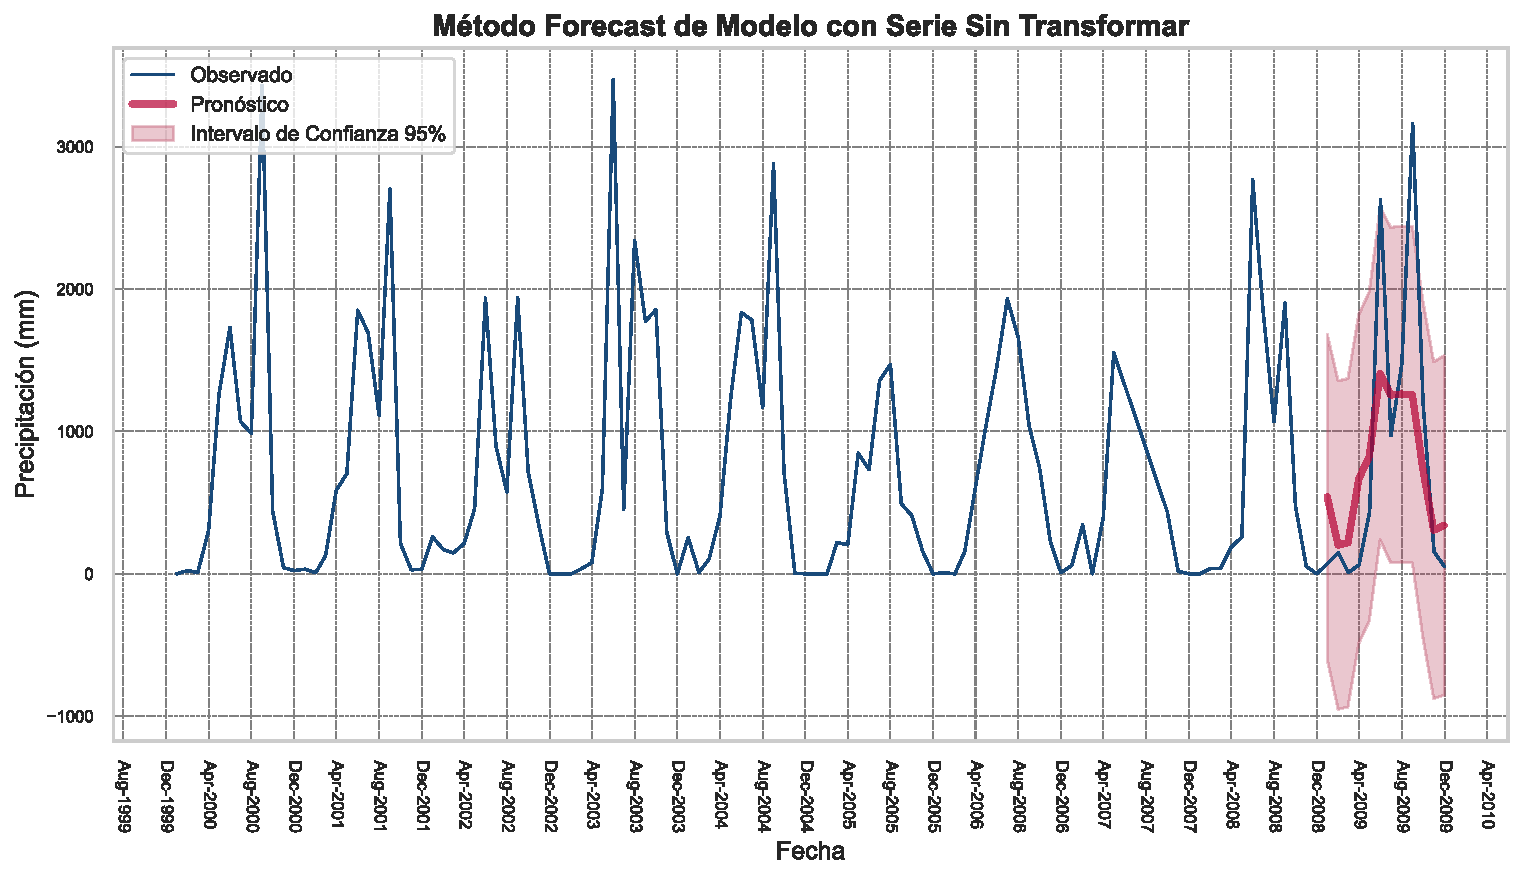
\includegraphics[width=0.8\textwidth]{imagenes/05-02-metodo-forecast-zoom.pdf}
    \caption{\textit{Elaboración Propia}. Método Forecast del Modelo con la Serie Sin Transformar}
\end{figure}

Se puede notar que el valor de octubre no está en el IC a un 95\%, esto ocurre seguramente porque el modelo no cuenta con una distribución normal en los residuos. 

\newpage
  \paragraph{Modelo Obtenido con la Serie Transformada}
  Obteniendo el pronóstico para los siguientes doce meses con el método forecast, desestandarizandolos y aplicando la transformación inversa de Yeo-Johnson, se obtuvieron los siguientes resultados: 

    \begin{table}[ht]
\centering
\footnotesize
\begin{tabular}{lrrrrrr}
\toprule
 & \textbf{Pronóstico} & \textbf{Límite Inferior} & \textbf{Límite Superior} & \textbf{Valor Observado} & \textbf{Residuos} \\
\midrule
2008-12-31 & 44.953714 & -1.768799 & 634.580471 & 74 & 29.046286 \\
2009-01-31 & 86.154521 & -1.056604 & 965.287325 & 148 & 61.845479 \\
2009-02-28 & 68.232307 & -1.477922 & 872.355113 & 8 & -60.232307 \\
2009-03-31 & 131.127054 & -0.297873 & 1260.040847 & 64 & -67.127054 \\
2009-04-30 & 428.426175 & 15.699218 & 2617.210481 & 436 & 7.573825 \\
2009-05-31 & 763.114253 & 47.562078 & 3972.644947 & 2627 & 1863.885747 \\
2009-06-30 & 779.087074 & 37.660483 & 4409.534391 & 972 & 192.912926 \\
2009-07-31 & 869.768181 & 43.029260 & 4890.317654 & 1474 & 604.231819 \\
2009-08-31 & 900.651856 & 44.624350 & 5062.589225 & 3161 & 2260.348144 \\
2009-09-30 & 485.254867 & 10.547197 & 3399.343448 & 1190 & 704.745133 \\
2009-10-31 & 155.744319 & -0.807449 & 1736.882669 & 155 & -0.744319 \\
2009-11-30 & 108.943275 & -1.512804 & 1460.964464 & 51 & -57.943275 \\
\bottomrule
\end{tabular}
\caption{\textit{Elaboración Propia}. Pronósticos, límites y residuos de la serie transformada}
\end{table}


\begin{figure}[ht]
    \centering
    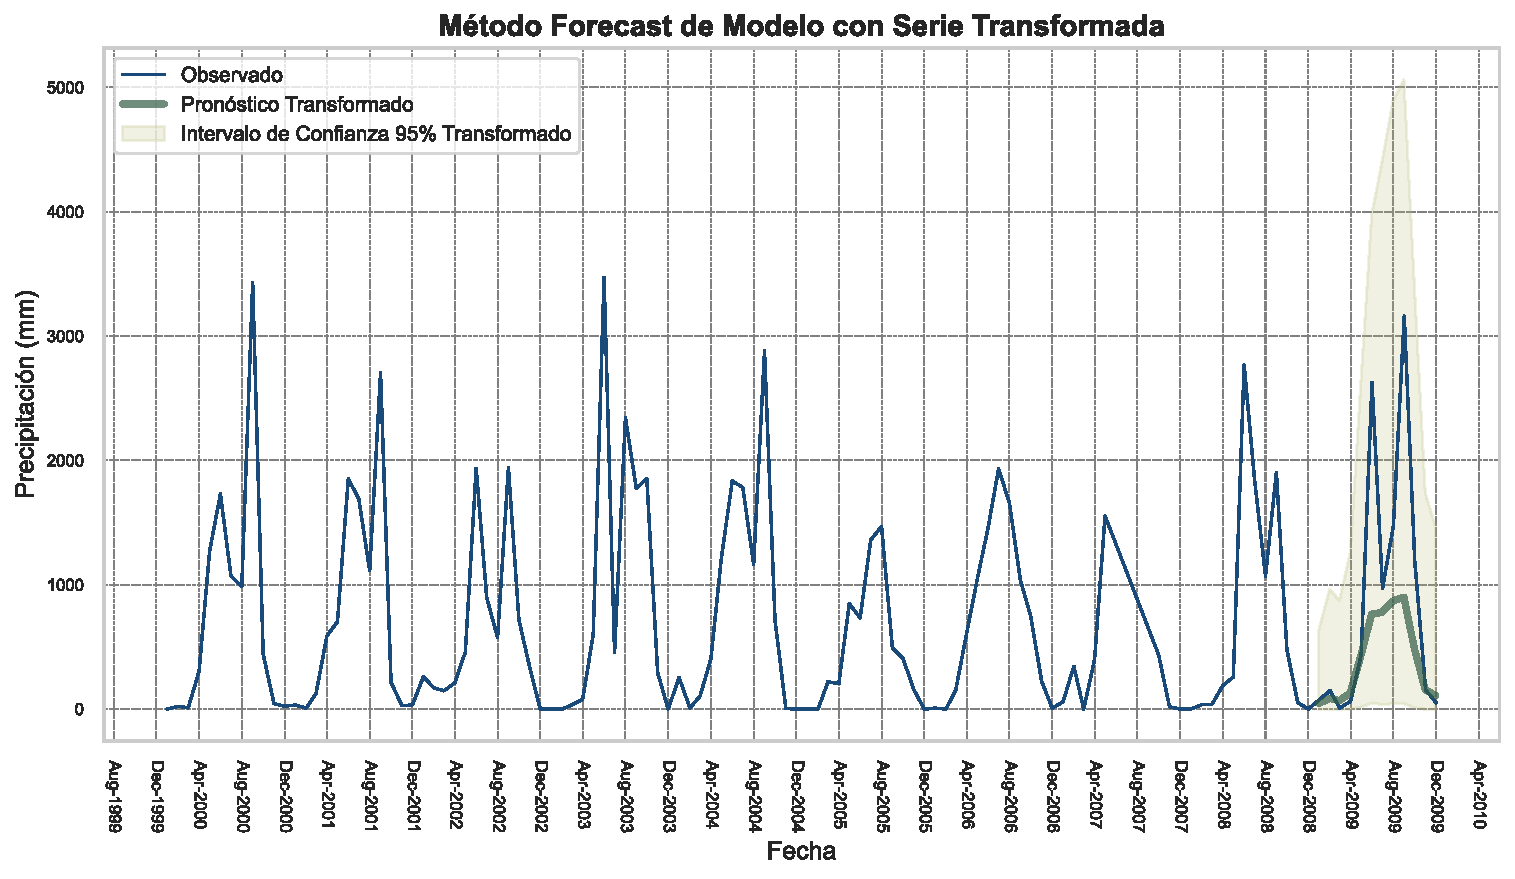
\includegraphics[width=0.8\textwidth]{imagenes/05-03-metodo-forecast-zoom.pdf}
    \caption{\textit{Elaboración Propia}. Método Forecast del Modelo con la Serie Transformada}
\end{figure}

Es interesante notar que en este modelo el intervalo de confianza apenas llega a ser negativo, esto puede ser debido a la normalidad en los residuos, sin embargo, no se esperaba un comportamiento tan "bueno"  del IC, ya que se creía que el estimador puntual sería incorrecto.

\newpage
  \paragraph{Comparación entre Ambos Modelos}

Se comparan ambos pronósticos, uno del modelo con la serie transformada y otro con el modelo de la serie sin transformar.

\begin{table}[ht]
\footnotesize
\centering
\begin{tabular}{lrrrrr}
\toprule
 & \textbf{Pronóstico} & \textbf{Pronóstico T} & \textbf{Valor Observado} & \textbf{Residuos} & \textbf{Residuos T} \\
\midrule
2008-12-31 & 44.953714 & 540.502158 & 74 & 29.046286 & -466.502158 \\
2009-01-31 & 86.154521 & 201.870616 & 148 & 61.845479 & -53.870616 \\
2009-02-28 & 68.232307 & 218.349640 & 8 & -60.232307 & -210.349640 \\
2009-03-31 & 131.127054 & 666.919279 & 64 & -67.127054 & -602.919279 \\
2009-04-30 & 428.426175 & 824.911936 & 436 & 7.573825 & -388.911936 \\
2009-05-31 & 763.114253 & 1406.446553 & 2627 & 1863.885747 & 1220.553447 \\
2009-06-30 & 779.087074 & 1256.178392 & 972 & 192.912926 & -284.178392 \\
2009-07-31 & 869.768181 & 1262.636919 & 1474 & 604.231819 & 211.363081 \\
2009-08-31 & 900.651856 & 1259.408611 & 3161 & 2260.348144 & 1901.591389 \\
2009-09-30 & 485.254867 & 736.647934 & 1190 & 704.745133 & 453.352066 \\
2009-10-31 & 155.744319 & 307.230864 & 155 & -0.744319 & -152.230864 \\
2009-11-30 & 108.943275 & 340.113522 & 51 & -57.943275 & -289.113522 \\
\bottomrule
\end{tabular}
\caption{\textit{Elaboración Propia}. Comparación entre Modelos}
\end{table}



\begin{figure}[ht]
    \centering
    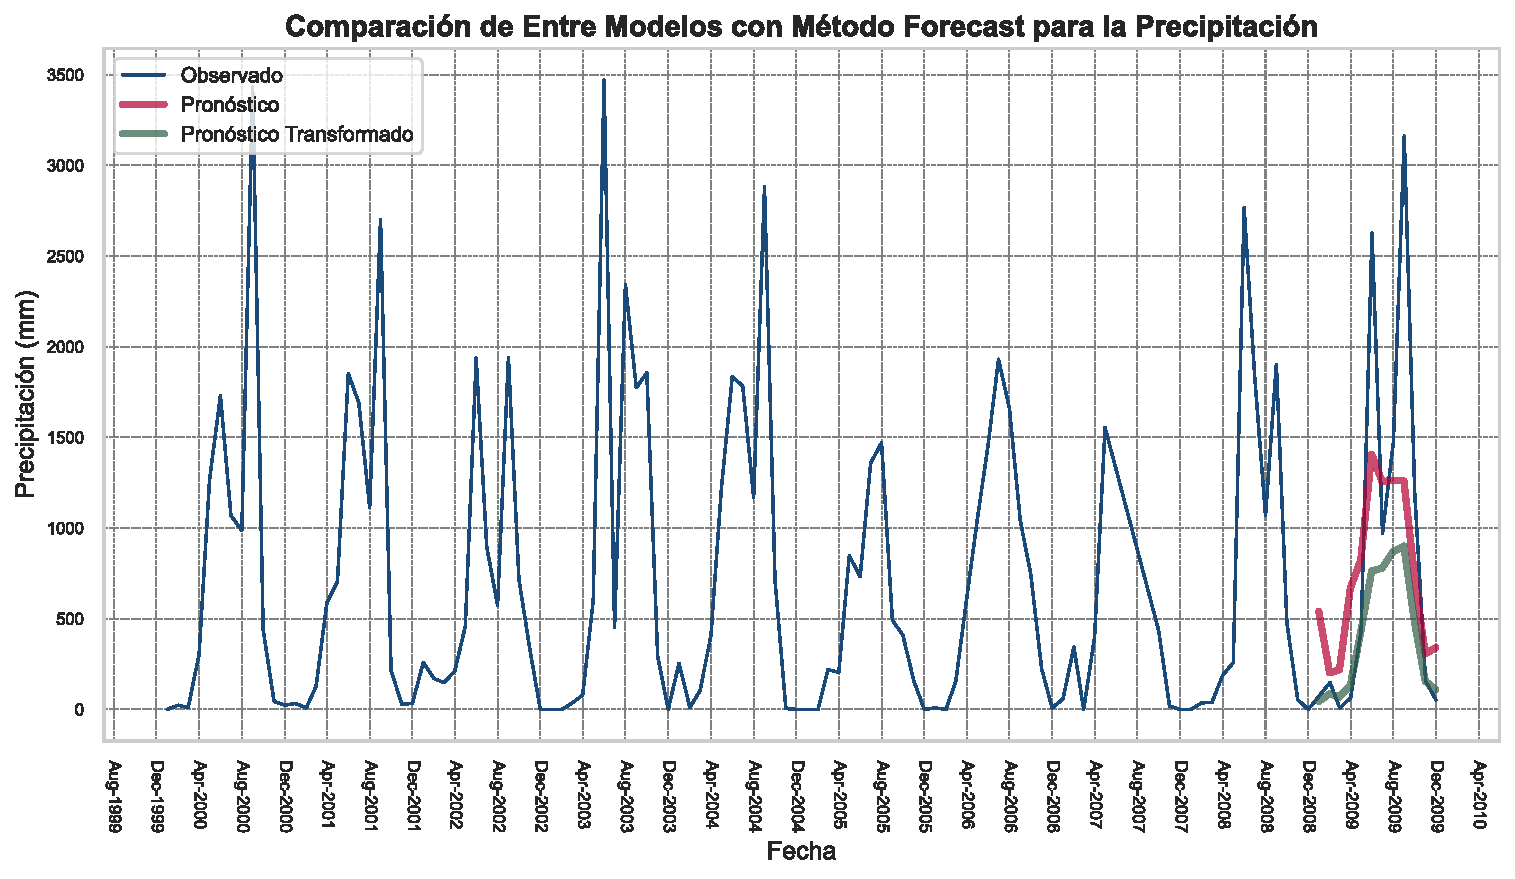
\includegraphics[width=0.8\textwidth]{imagenes/05-04-metodo-forecast-comparacion.pdf}
    \caption{\textit{Elaboración Propia}. Comparación entre Modelos}
\end{figure}

Se observa que, en cuanto a estimación puntual, el modelo sin transformaciones se encuentra siempre con valores más positivos que el modelo que se entrenó con transformaciones, teniendo residuos más bajos en temporadas con alta precipitación, y el otro al revés.

















\newpage
  \subsubsection{Pronóstico Óptimo}

El pronóstico óptimo se calcula únicamente para el primer modelo.

\[
\text{ARIMA}(13,0,0) \times (0,1,4)_{12} \text{ para } X_t
\]

con coeficientes:
\vspace{-10pt}
\begin{align*}
\phi_1 &= 0.136917, & \phi_2 &= 0.019014, & \phi_3 &= -0.050067, \\
\phi_4 &= 0.069698, & \phi_5 &= 0.111714, & \phi_6 &= 0.110100, \\
\phi_7 &= 0.010426, & \phi_8 &= 0.051137, & \phi_9 &= -0.033088, \\
\phi_{10} &= 0.009268, & \phi_{11} &= -0.103359, & \phi_{12} &= -0.538506, \\
\phi_{13} &= 0.046024, & \Theta_1 &= 1.375601, & \Theta_2 &= -0.367441, \\
\Theta_3 &= -0.097350, & \Theta_4 &= 0.078355
\end{align*}


\paragraph{Desarrollo para el Pronóstico Óptimo}



El modelo puede representarse como:

\[
\Phi_0(B^{12}) \phi_{13}(B) \nabla_{12} X_t = \Theta_4(B^{12}) \varepsilon_t,\quad \varepsilon_t \sim \mathcal{N}(0, 1)
\]


\noindent Lado izquierdo:
\[
(1 - \phi_1 B - \cdots - \phi_{13} B^{13})(X_t - X_{t-12}) = X_t - X_{t-12} - \sum_{h=1}^{13} \phi_h (X_{t-h} - X_{t-h-12})
\]

\noindent Lado derecho:
\[
(1 - \Theta_1 B^{12} - \Theta_2 B^{24} - \Theta_3 B^{36} - \Theta_4 B^{48}) \varepsilon_t = \varepsilon_t - \sum_{j=1}^4 \Theta_j \varepsilon_{t - 12j}
\]

\noindent Despejando \( X_t \):

\[
X_t = X_{t-12} + \sum_{k=1}^{13} \phi_k (X_{t-k} - X_{t-k-12}) + \varepsilon_t - \sum_{j=1}^4 \Theta_j \varepsilon_{t - 12j}
\]

\noindent Por lo que, el pronóstico óptimo es:

\[
X_t(h) = \mathbb{E}_t[X_{t+h-12}] + \sum_{k=1}^{13} \phi_k \left( \mathbb{E}_t[X_{t+h-k}] - \mathbb{E}_t[X_{t+h-k-12}] \right) + \mathbb{E}_t[\varepsilon_{t+h}] - \sum_{j=1}^{4} \Theta_j \mathbb{E}_t[\varepsilon_{t+h - 12j}]
\]


\paragraph{Resultados del Pronóstico Óptimo}
Una vez sumado el polinomio de 32 términos, se obtienen los siguientes resultados
\begin{align*}
X_{672}(1)  &= -0.0597 \\
X_{672}(2)  &= -0.6402 \\
X_{672}(3)  &= -0.3030 \\
X_{672}(4)  &= 0.0024 \\
X_{672}(5)  &= 0.0789 \\
X_{672}(6)  &= 1.2996 \\
X_{672}(7)  &= 2.0781 \\
X_{672}(8)  &= 1.0283 \\
X_{672}(9)  &= 0.3826 \\
X_{672}(10) &= 0.6342 \\
X_{672}(11) &= -0.0721 \\
X_{672}(12) &= -1.1106
\end{align*}


  \paragraph{Intervalo de Confianza}
Ya que tenemos el pronóstico óptimo (estandarizado) se obtienen los intervalos de confianza. Dado que \( \text{Var}(X_t(h)) = \left( \sum_{j=0}^h \psi_j^2 \right) \sigma^2 \), los intervalos de confianza al 95\% son:

\[
X_t(h) \pm Z_{\frac{\alpha}{2}} \cdot \sqrt{ \sum_{j=0}^{h} \psi_j^2 } \cdot \hat{\sigma}_\varepsilon
\]

donde los \( \psi_j \) se calculan mediante la recursión:

\begin{itemize}
    \item \( \psi_0 = -1 \)
    \item \( \psi_i = \theta_i + \sum_{k=1}^{i} \Phi_k \psi_{i-k} \) si \( i \leq q \)
    \item \( \psi_i = \sum_{k=1}^{p+d} \Phi_k \psi_{i-k} \) si \( i > q \)
\end{itemize}

      \subparagraph{Cálculo de las $\psi$}
      Se calculan las $\psi$
      \vspace{-20pt}
    \begin{align*}
\psi_0 &= -1 \\
\psi_1 &= -0.14196630827330695 \\
\psi_2 &= -0.0012833831644303538 \\
\psi_3 &= -0.04711945564958303 \\
\psi_4 &= 0.055666495988799594 \\
\psi_5 &= 0.13168502721815675 \\
\psi_6 &= 0.14390060444632985 \\
\psi_7 &= 0.05528005326826947 \\
\psi_8 &= 0.06597563860600197 \\
\psi_9 &= -0.023742200999115167 \\
\psi_{10} &= -0.029931708277211113 \\
\psi_{11} &= -0.13198547391317694 \\
\psi_{12} &= 0.7710272345141591
\end{align*}




    \subparagraph{Desviación Estándar del Ruido Blanco}
    Se obtiene la desviación estándar del ruido blanco,
$\sigma=0.6807672997433546$.










  


    
    \subparagraph{Intervalos de Predicción}

Se calculan los intervalos de predicción de la siguiente forma, con $\alpha=0.95$:
    \[
X_t(h) \pm Z_{\frac{\alpha}{2}} \cdot \sqrt{ \sum_{j=0}^{h} \psi_j^2 } \cdot \hat{\sigma}_\varepsilon
\]

Obteniendo los siguientes resultados:
\begin{align*}
\text{Intervalo 1:} &\quad (-1.393982459496975, 1.2746253554969749) \\
\text{Intervalo 2:} &\quad (-1.9878485554111043, 0.7075172474111042) \\
\text{Intervalo 3:} &\quad (-1.6506852053494947, 1.0446827733494948) \\
\text{Intervalo 4:} &\quad (-1.3467435497585691, 1.3515559017585692) \\
\text{Intervalo 5:} &\quad (-1.2722535341171932, 1.4301320121171934) \\
\text{Intervalo 6:} &\quad (-0.06293200205383043, 2.6622066420538304) \\
\text{Intervalo 7:} &\quad (0.7020341131440195, 3.45409653885598) \\
\text{Intervalo 8:} &\quad (-0.349748182450476, 2.406265238450476) \\
\text{Intervalo 9:} &\quad (-0.9982177354298769, 1.7634137014298767) \\
\text{Intervalo 10:} &\quad (-0.7469687343170736, 2.0153894083170734) \\
\text{Intervalo 11:} &\quad (-1.4538500316205047, 1.3096627116205048) \\
\text{Intervalo 12:} &\quad (-2.5035084583313623, 0.2823594183313627)
\end{align*}

\subparagraph{Desestandarización}

Desestandarizamos con $\mu = 784.0136363636364, \quad\sigma= 880.4446163963537$ .

si \(z\) representa un pronóstico,

\[
z = X_t(h) \pm Z_{\frac{\alpha}{2}} \cdot \sqrt{ \sum_{j=0}^{h} \psi_j^2 } \cdot \hat{\sigma}_\varepsilon
\]
se desestandariza así:

\[
x = z \cdot \sigma + \mu
\]
y \( x \) representa el valor en la escala original. 

Se aplica el mismo procedimiento para el intervalo de confianza.

\newpage
\subparagraph{Resultados}
Se obtienen los siguientes resultados del pronóstico óptimo.

\begin{table}[ht]
\footnotesize
\centering
\begin{tabular}{lrrrrrr}
\toprule
 & \textbf{Pronóstico} & \textbf{Límite Inferior} & \textbf{Límite Superior} & \textbf{Valor Observado} & \textbf{Residuos} \\
\midrule
2008-12-31 & 731.469977 & -443.310715 & 1906.250669 & 74 & -657.469977 \\
2009-01-31 & 220.383233 & -966.176922 & 1406.943388 & 148 & -72.383233 \\
2009-02-28 & 517.237847 & -669.323266 & 1703.798960 & 8 & -509.237847 \\
2009-03-31 & 786.132141 & -401.719472 & 1973.983754 & 64 & -722.132141 \\
2009-04-30 & 853.515264 & -336.135138 & 2043.165667 & 436 & -417.515264 \\
2009-05-31 & 1928.272318 & 728.605494 & 3127.939142 & 2627 & 698.727682 \\
2009-06-30 & 2613.635065 & 1402.115792 & 3825.154339 & 972 & -1641.635065 \\
2009-07-31 & 1689.338322 & 476.079732 & 2902.596911 & 1474 & -215.338322 \\
2009-08-31 & 1120.869971 & -94.861795 & 2336.601736 & 3161 & 2040.130029 \\
2009-09-30 & 1342.400713 & 126.349036 & 2558.452391 & 1190 & -152.400713 \\
2009-10-31 & 720.539162 & -496.020797 & 1937.099120 & 155 & -565.539162 \\
2009-11-30 & -193.785721 & -1420.186908 & 1032.615466 & 51 & 244.785721 \\
\bottomrule
\end{tabular}
\caption{\textit{Elaboración Propia}. Pronósticos, límites y residuos del cálculo del pronóstico óptimo}
\end{table}


\begin{figure}[ht]
    \centering
    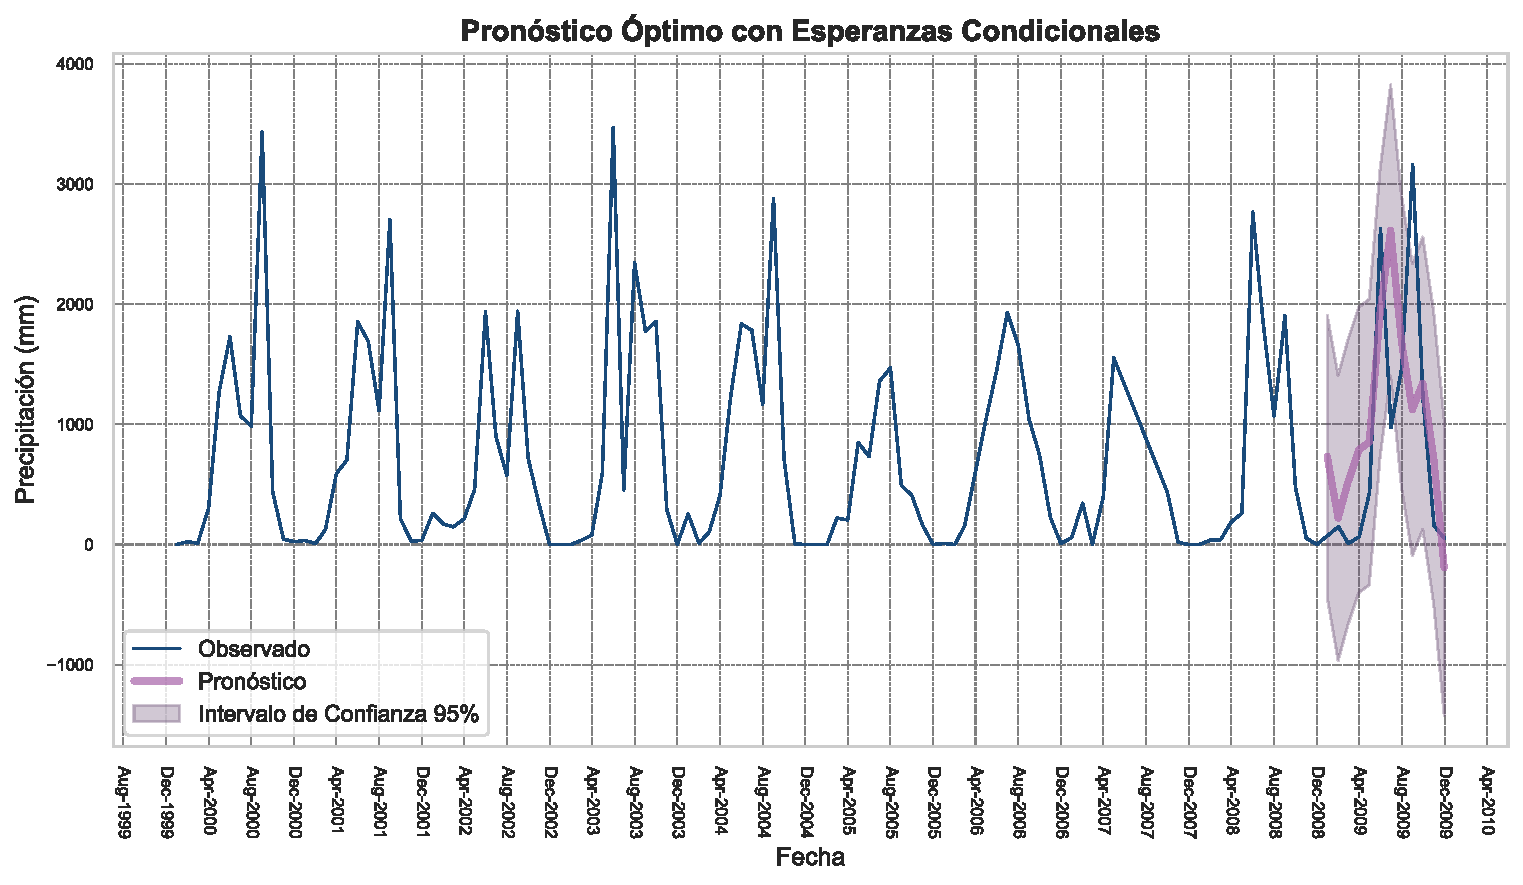
\includegraphics[width=0.8\textwidth]{imagenes/05-03-pronostico-optimo.pdf}
    \caption{\textit{Elaboración Propia}. Pronóstico Óptimo con Esperanzas Condicionales}
\end{figure}

En la Figura 29 se nota la importancia de que el modelo cumpla el supuesto de normalidad en los residuos, podemos ver que, otra vez, en octubre de 2009 se encuentra una observación que está fuera del intervalo de confianza. Por cómo está definido el modelo, con 13 parámetros autorregresivos, se nota que el pronóstico es demasiado parecido a las observaciones del año anterior, esta vez teniendo el pico de septiembre bajo, debido a que en años anteriores no llovió durante esas fechas.



\newpage
\subparagraph{Comparación}
En esta sección se comparan los resultados del método forecast y del pronóstico óptimo.
\begin{table}[ht]
\tiny
\centering
\begin{tabular}{lrrrrrr}
\toprule
 & \textbf{Pronóstico Óptimo} & \textbf{Método Forecast} & \textbf{Valor Observado} & \textbf{Residuos Óptimo} & \textbf{Residuos Forecast} \\
\midrule
2008-12-31 & 731.469977 & 540.502158 & 74 & -657.469977 & -466.502158 \\
2009-01-31 & 220.383233 & 201.870616 & 148 & -72.383233 & -53.870616 \\
2009-02-28 & 517.237847 & 218.349640 & 8 & -509.237847 & -210.349640 \\
2009-03-31 & 786.132141 & 666.919279 & 64 & -722.132141 & -602.919279 \\
2009-04-30 & 853.515264 & 824.911936 & 436 & -417.515264 & -388.911936 \\
2009-05-31 & 1928.272318 & 1406.446553 & 2627 & 698.727682 & 1220.553447 \\
2009-06-30 & 2613.635065 & 1256.178392 & 972 & -1641.635065 & -284.178392 \\
2009-07-31 & 1689.338322 & 1262.636919 & 1474 & -215.338322 & 211.363081 \\
2009-08-31 & 1120.869971 & 1259.408611 & 3161 & 2040.130029 & 1901.591389 \\
2009-09-30 & 1342.400713 & 736.647934 & 1190 & -152.400713 & 453.352066 \\
2009-10-31 & 720.539162 & 307.230864 & 155 & -565.539162 & -152.230864 \\
2009-11-30 & -193.785721 & 340.113522 & 51 & 244.785721 & -289.113522 \\
\bottomrule
\end{tabular}
\caption{\textit{Elaboración Propia}. Comparación entre el pronóstico óptimo y el método Forecast, junto con sus respectivos residuos}
\end{table}


\begin{figure}[ht]
    \centering
    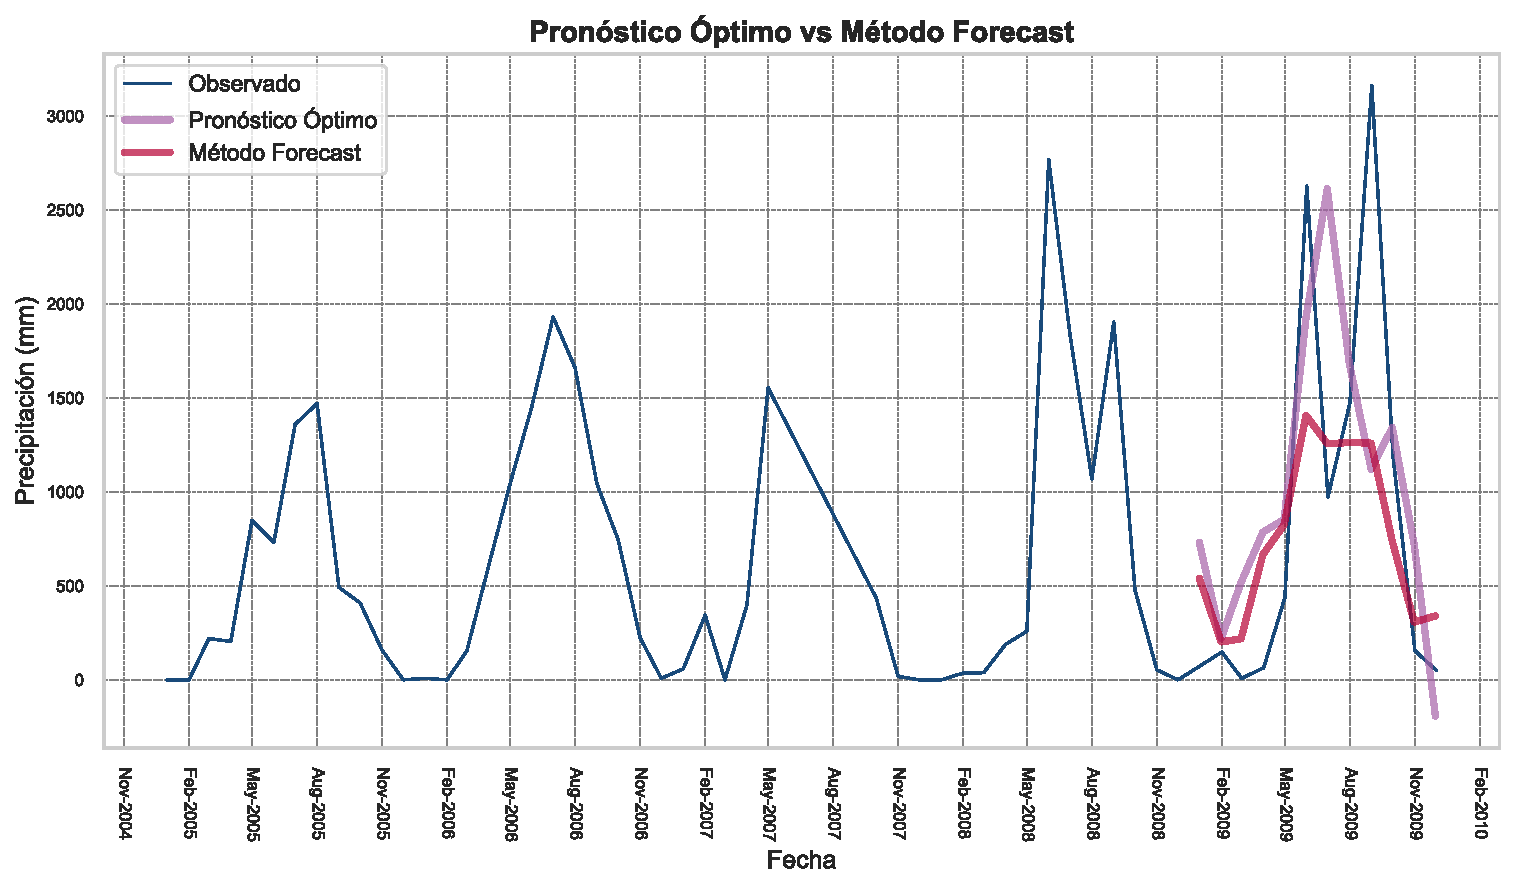
\includegraphics[width=0.8\textwidth]{imagenes/05-04-comparacion.pdf}
    \caption{\textit{Elaboración Propia}. Comparación de Pronóstico Óptimo contra Método Forecast}
\end{figure}

Se puede notar que de ambas maneras se consigue un tipo de pronóstico estacional que tiene sus valores más altos durante el periodo de verano. En el cuadro 18, se puede ver que el método forecast tiene menores residuos a futuro que el método de pronóstico óptimo, indicando un mejor ajuste.






  
\newpage

\subsection{Actualización de Pronóstico}
En esta sección se agrega el valor de diciembre de 2008, 74 estandarizado, y se realiza la actualización de pronóstico con el método forecast y de la manera en que se abordó en clase para luego compararlos.









\subsubsection{Método Forecast}

En esta sección se realiza la actualización de pronóstico con el método forecast, donde se obtuvieron los siguientes resultados:

\begin{table}[ht]
\tiny
\centering
\begin{tabular}{lrrrrrr}
\toprule
 & \textbf{Pronóstico} & \textbf{Pronóstico Actualizado} & \textbf{Valor Observado} & \textbf{Residuos} & \textbf{Residuos Actualizados} \\
\midrule
2009-01-31 & 201.870616 & 135.678753 & 148 & -53.870616 & 12.321247 \\
2009-02-28 & 218.349640 & 217.762493 & 8 & -210.349640 & -209.762493 \\
2009-03-31 & 666.919279 & 644.960938 & 64 & -602.919279 & -580.960938 \\
2009-04-30 & 824.911936 & 850.856468 & 436 & -388.911936 & -414.856468 \\
2009-05-31 & 1406.446553 & 1467.835729 & 2627 & 1220.553447 & 1159.164271 \\
2009-06-30 & 1256.178392 & 1323.237743 & 972 & -284.178392 & -351.237743 \\
2009-07-31 & 1262.636919 & 1288.347469 & 1474 & 211.363081 & 185.652531 \\
2009-08-31 & 1259.408611 & 1290.129012 & 3161 & 1901.591389 & 1870.870988 \\
2009-09-30 & 736.647934 & 725.578659 & 1190 & 453.352066 & 464.421341 \\
2009-10-31 & 307.230864 & 293.280258 & 155 & -152.230864 & -138.280258 \\
2009-11-30 & 340.113522 & 278.605347 & 51 & -289.113522 & -227.605347 \\
\bottomrule
\end{tabular}
\caption{\textit{Elaboración Propia}. Comparación entre el pronóstico, el pronóstico actualizado, los valores reales y los residuos}
\end{table}



\begin{figure}[ht]
    \centering
    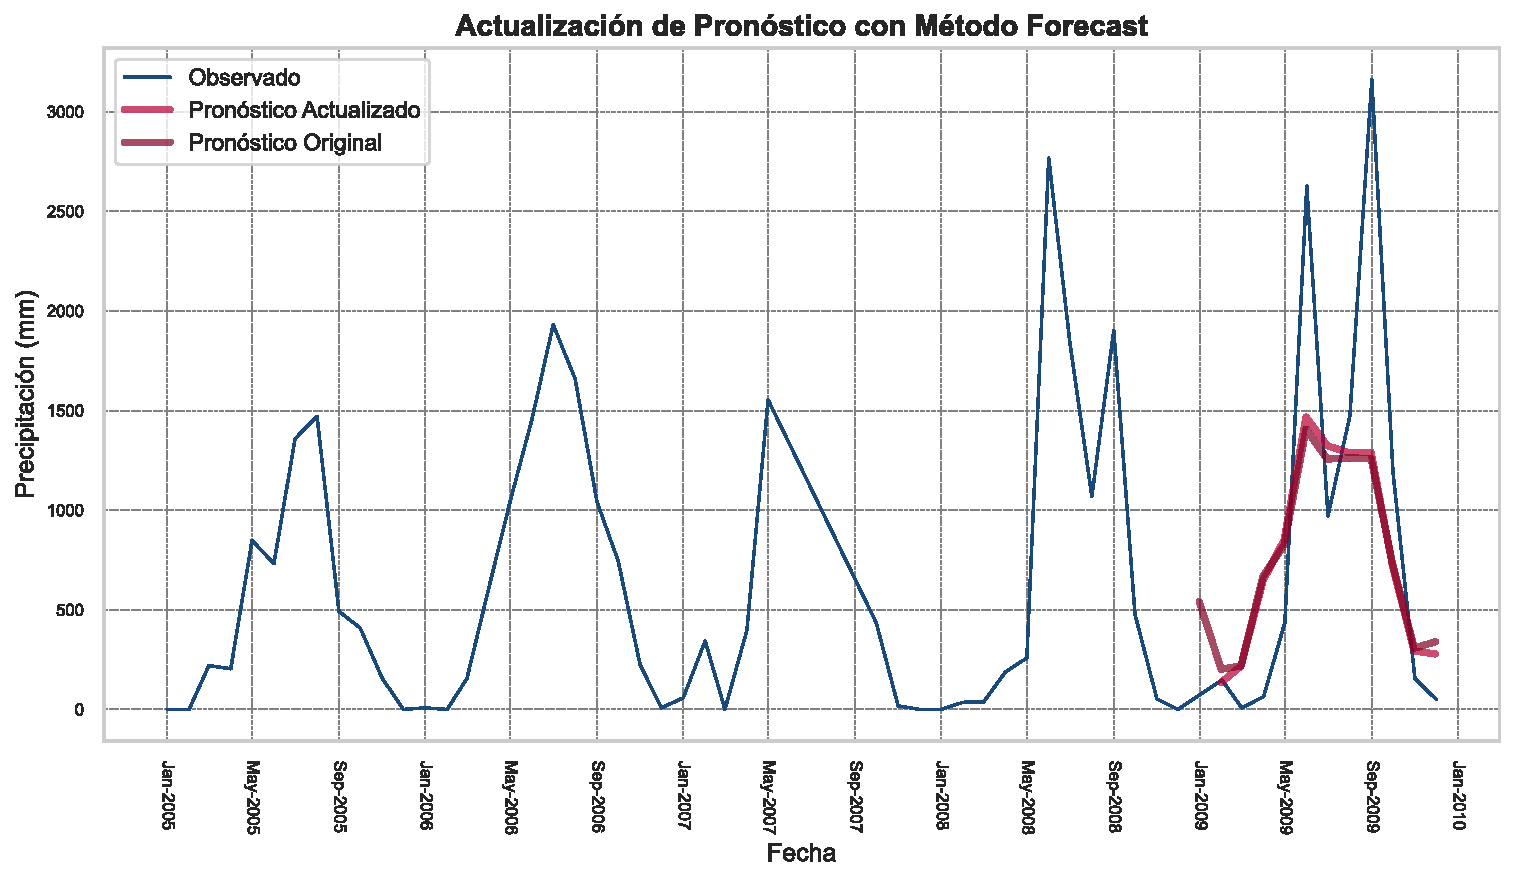
\includegraphics[width=0.8\textwidth]{imagenes/06-01-Actualizacion-de-pronostico-metodo-forecast.pdf}
    \caption{\textit{Elaboración Propia}. Actualización del Pronóstico con Método Forecast}
\end{figure}

Se observa que en general, aunque los cambios sean mínimos, los residuos a futuro son más pequeños una vez que se ha actualizado el pronóstico, pero casi no hay diferencia en la forma de la serie. 

\newpage
$\quad$
\subsubsection{Actualización de Pronóstico}
En esta sección se muestra la actualización de pronóstico realizada en Excel.

\begin{table}[ht]
\tiny
\centering
\begin{tabular}{lrrrrr}
\toprule
 & \textbf{Pronóstico Óptimo} & \textbf{Pronóstico Actualizado} & \textbf{Valor Observado} & \textbf{Residuos Óptimo} & \textbf{Residuos Actualizado} \\
\midrule
2008-12-31 & 731.469977 & 74.000000 & 74 & -657.469977 & 0.000000 \\
2009-01-31 & 220.383233 & 127.044647 & 148 & -72.383233 & 20.955353 \\
2009-02-28 & 517.237847 & 516.394061 & 8 & 509.237847 & 508.394061 \\
2009-03-31 & 786.132141 & 755.152514 & 64 & 722.132141 & 691.152514 \\
2009-04-30 & 853.515264 & 890.114314 & 436 & 417.515264 & 454.114314 \\
2009-05-31 & 1928.272318 & 2014.851270 & 2627 & -698.727682 & -612.148730 \\
2009-06-30 & 2613.635065 & 2708.245392 & 972 & 1641.635065 & 1736.245392 \\
2009-07-31 & 1689.338322 & 1725.683297 & 1474 & 215.338322 & 251.683297 \\
2009-08-31 & 1120.869971 & 1164.246972 & 3161 & -2040.130029 & -1996.753028 \\
2009-09-30 & 1342.400713 & 1326.790929 & 1190 & 152.400713 & 136.790929 \\
2009-10-31 & 720.539162 & 700.859962 & 155 & 565.539162 & 545.859962 \\
2009-11-30 & -193.785721 & -280.562207 & 51 & -244.785721 & -331.562207 \\
\bottomrule
\end{tabular}
\caption{\textit{Elaboración Propia}. Comparación entre el pronóstico óptimo, el pronóstico actualizado y los residuos correspondientes}
\end{table}


\begin{figure}[ht]
    \centering
    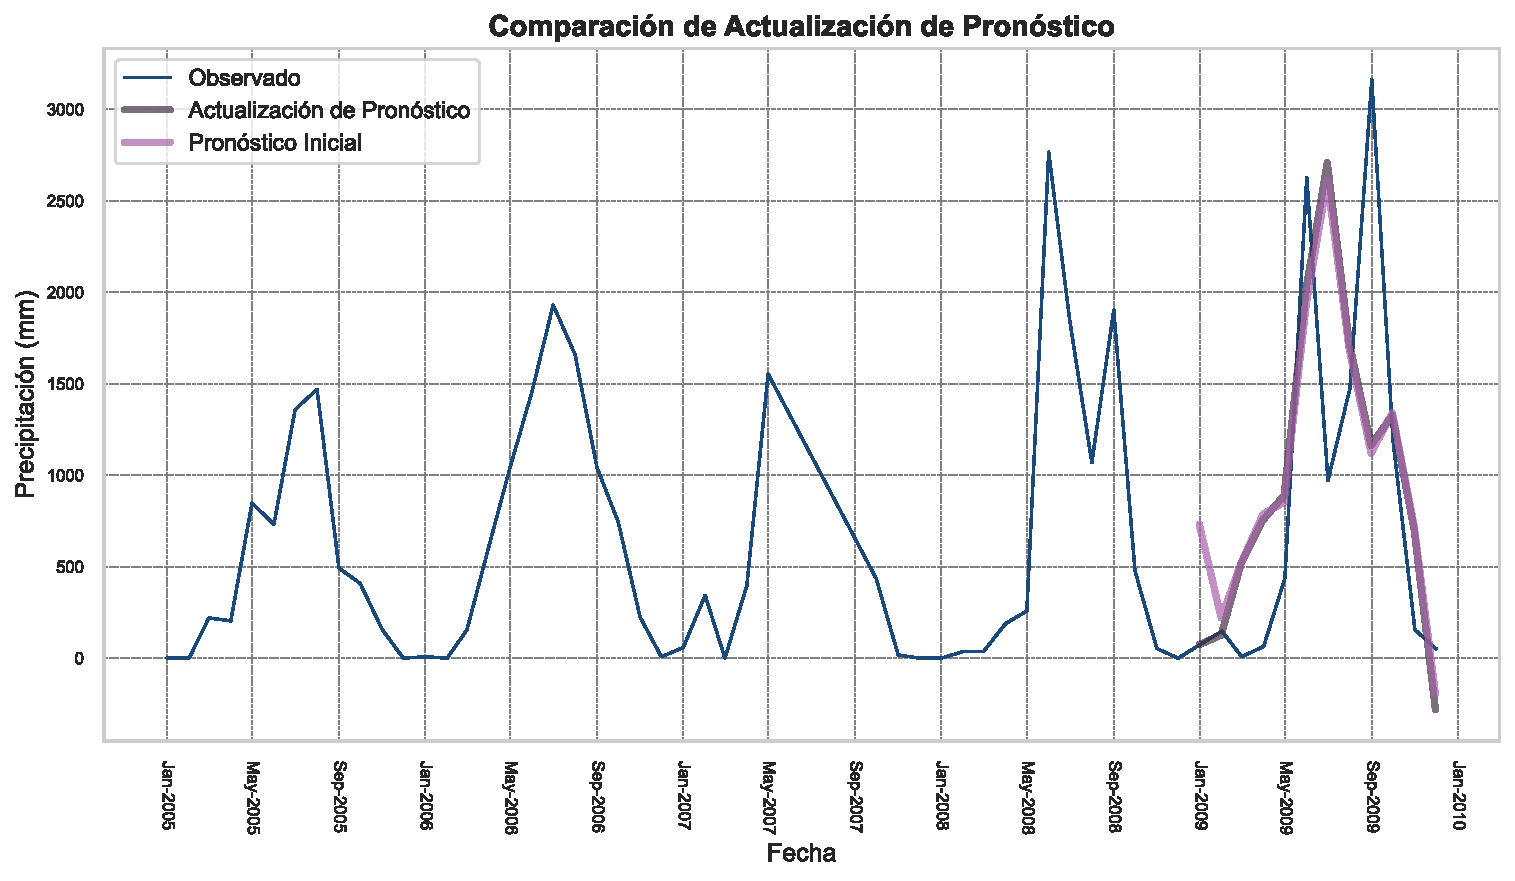
\includegraphics[width=0.8\textwidth]{imagenes/06-02-Actualizacion-de-pronostico.pdf}
    \caption{\textit{Elaboración Propia}. Actualización del Pronóstico}
\end{figure}

Ocurre lo mismo que en el caso pasado, una vez actualizado y generando pequeños cambios sin cambiar su forma, el pronóstico los residuos a futuro son menores, excepto en los meses de junio y julio.


\newpage
\subsubsection{Comparación}
En esta sección se comparan los resultados obtenidos luego de actualizar el pronóstico con el método forecast y con actualización del pronóstico.
\begin{table}[ht]
\tiny
\centering
\begin{tabular}{lrrrrr}
\toprule
 & \textbf{Pronóstico Actualizado} & \textbf{Método Forecast Actualizado} & \textbf{Valor Observado} & \textbf{Residuo Óptimo} & \textbf{Residuo Forecast} \\
\midrule
2008-12-31 & 74.000000 & NaN & 74 & 0.000 & NaN \\
2009-01-31 & 127.044647 & 201.870616 & 148 & 20.955 & -53.871 \\
2009-02-28 & 516.394061 & 218.349640 & 8 & -508.394 & -210.350 \\
2009-03-31 & 755.152514 & 666.919279 & 64 & -691.153 & -602.919 \\
2009-04-30 & 890.114314 & 824.911936 & 436 & -454.114 & -388.912 \\
2009-05-31 & 2014.851270 & 1406.446553 & 2627 & 612.149 & 1220.553 \\
2009-06-30 & 2708.245392 & 1256.178392 & 972 & -1736.245 & -284.178 \\
2009-07-31 & 1725.683297 & 1262.636919 & 1474 & -251.683 & 211.363 \\
2009-08-31 & 1164.246972 & 1259.408611 & 3161 & 1996.753 & 1901.591 \\
2009-09-30 & 1326.790929 & 736.647934 & 1190 & -136.791 & 453.352 \\
2009-10-31 & 700.859962 & 307.230864 & 155 & -545.860 & -152.231 \\
2009-11-30 & -280.562207 & 340.113522 & 51 & 331.562 & -289.114 \\
\bottomrule
\end{tabular}
\caption{\textit{Elaboración Propia}. Comparación entre el pronóstico óptimo actualizado, el método forecast actualizado, los valores reales y sus residuos.}
\end{table}

\begin{figure}[ht]
    \centering
    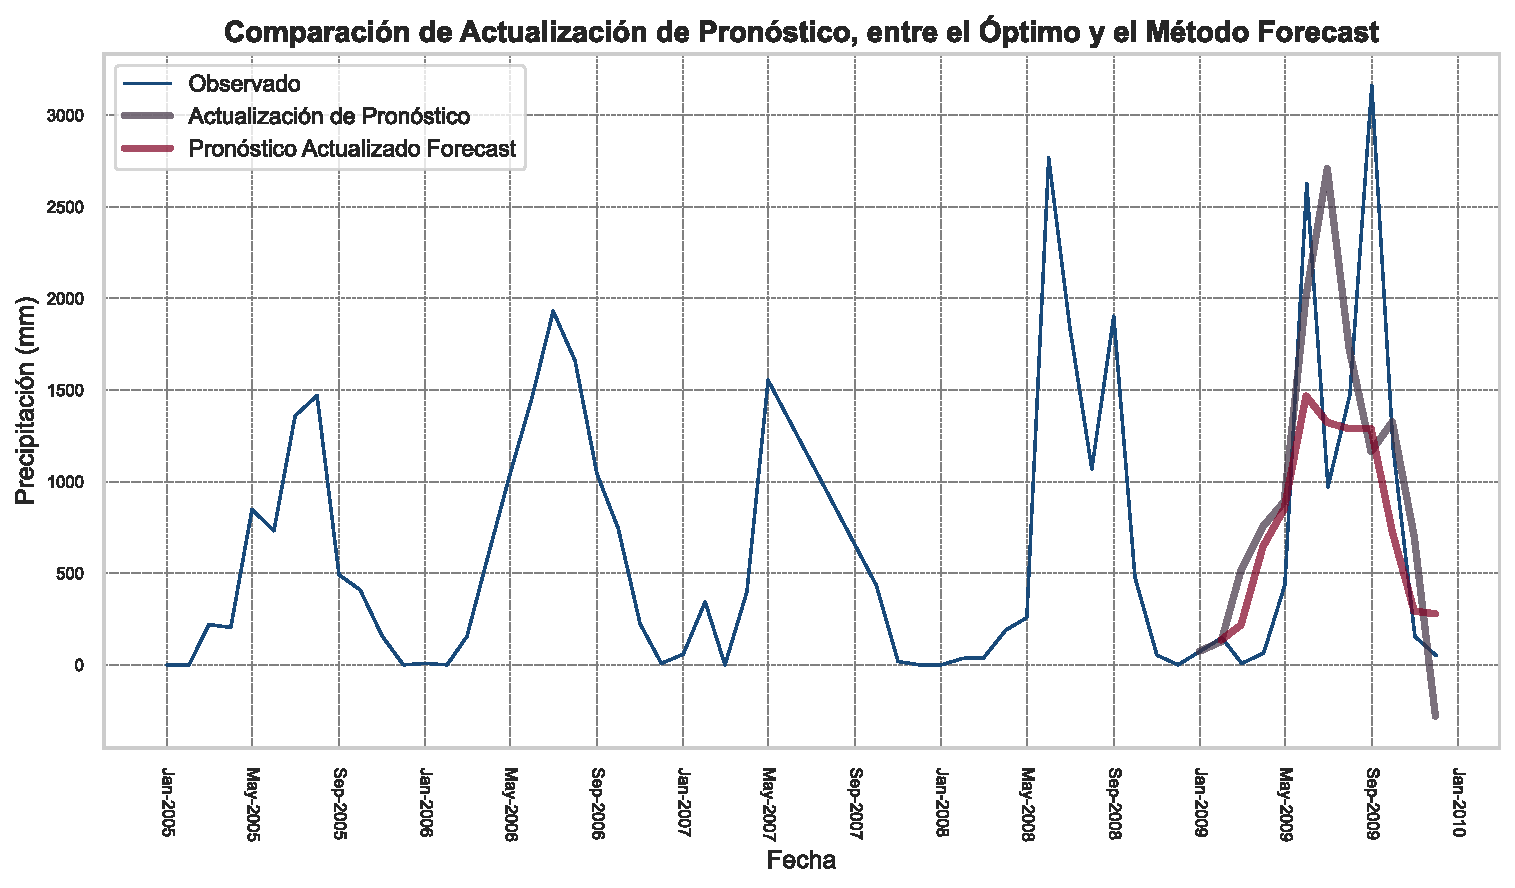
\includegraphics[width=0.8\textwidth]{imagenes/06-03-Actualizacion-de-pronostico-comparacion.pdf}
    \caption{\textit{Elaboración Propia}. Comparación de Actualización de Pronóstico con Método Forecast}
\end{figure}

Se puede notar que ambos se acercan más al valor real una vez actualizados, ya que sus residuos son más pequeños esta vez. No hay uno que sea significativamente mejor que el otro luego de la actualización de pronóstico, ya que hay meses en los que el método forecast se acerca más que el método de actualización de pronóstico y viceversa.








































\newpage
\section{Conclusiones}

Aunque es cierto que la precipitación mensual tiene estacionalidad cada 12 meses y una estacionariedad general, no se pudo encontrar un modelo adecuado que cumpliera todos los supuestos.

 El modelo que se entrenó sin transformación tuvo como ventaja que no se alteró la distribución original, su desventaja crítica es que los residuos no cumplen normalidad, lo que invalida intervalos de confianza. Como sus residuos presenten colas pesadas, los residuos extremos estarán subestimados, (como se observa en la Figura 26 y 29, donde una observación real queda fuera del intervalo al 95\%) demostrando que no se puede confiar plenamente en los intervalos de confianza de este modelo. Sin embargo, aunque no cumple el supuesto de normalidad en, se siguen teniendo pronósticos óptimos cercanos a la realidad.
 
 El modelo entrenado con la serie que tiene la transformación Yeo–Johnson tiene como ventaja que los residuos sí cumplen normalidad, sus desventajas residuales son la no independencia y la falta de heterocedasticidad, donde la amplitud de los residuos varía a lo largo del tiempo, esto significa que seguimos violando supuestos de independencia y varianza constante, por lo que los residuos de predicción no son verdaderamente ruido blanco, ademas de todavía contener información importante sobre la serie. Tampoco se puede confiar absolutamente en estos intervalos de confianza en el pronóstico, ya que asumen varianza constante, de modo que los intervalos de confianza pueden ser demasiado estrechas o demasiado anchas en distintas épocas, lo que también compromete la validez de la inferencia. 


 El método forecast y el método de pronóstico óptimo con esperanzas condicionales son herramientas capaces de predecir el comportamiento de la serie de tiempo. El pronóstico óptimo basado en esperanzas condicionales tiende a capturar con mayor fidelidad los picos extremos y a ofrecer ajustes más coherentes con los parámetros estimados, frente al método forecast. Esto hace que, en aplicaciones donde la interpretabilidad y la lógica del modelo sean prioritarias, se prefiera el pronóstico óptimo.


Para tener un modelo plenamente confiable, se tendría que encontrar un mejor ARIMA que capture toda la temporalidad de la serie. Ninguno de los dos enfoques cumple con todos los supuestos que un modelo debería tener; el modelo sin transformación falla en normalidad y el modelo con transformación incurre en dependencia, heterogeneidad de varianza, y su media. Para alcanzar un modelo plenamente confiable, será necesario explorar especificaciones más parsimoniosas que satisfagan simultáneamente los requisitos de normalidad, independencia y homocedasticidad de los residuos, sin sacrificar la capacidad predictiva.






\newpage
\section{Referencias}


In‐Kwon Yeo, Richard A. Johnson, A new family of power transformations to improve normality or symmetry, Biometrika, Volume 87, Issue 4, December 2000, Pages 954–959, https://doi.org/10.1093/biomet/87.4.954

National Centers for Environmental Information. (2018). GHCN monthly precipitation dataset (version 4). NOAA. https://www.ncei.noaa.gov/data/ghcnm/v4/precipitation/



\end{document}



